%%% The main file. It contains definitions of basic parameters and includes all other parts.

% Meta-data of your thesis (please edit)
\input metadata.tex

% Generate metadata in XMP format for use by the pdfx package
\input xmp.tex

%% Settings for single-side (simplex) printing
% Margins: left 40mm, right 25mm, top and bottom 25mm
% (but beware, LaTeX adds 1in=25.4mm implicitly)
\documentclass[12pt,a4paper]{report}
\setlength\textwidth{145mm}
\setlength\textheight{247mm}
\setlength\oddsidemargin{14.6mm}
\setlength\evensidemargin{14.6mm}
\setlength\topmargin{0mm}
\setlength\headsep{0mm}
\setlength\headheight{0mm}
% \openright makes the following text appear on a right-hand page
\let\openright=\clearpage

%% Settings for two-sided (duplex) printing
% \documentclass[12pt,a4paper,twoside,openright]{report}
% \setlength\textwidth{145mm}
% \setlength\textheight{247mm}
% \setlength\oddsidemargin{14.6mm}
% \setlength\evensidemargin{0mm}
% \setlength\topmargin{0mm}
% \setlength\headsep{0mm}
% \setlength\headheight{0mm}
% \let\openright=\cleardoublepage

%% If the thesis has no printed version, symmetric margins look better
% \documentclass[12pt,a4paper]{report}
% \setlength\textwidth{145mm}
% \setlength\textheight{247mm}
% \setlength\oddsidemargin{7.1mm}
% \setlength\evensidemargin{7.1mm}
% \setlength\topmargin{0mm}
% \setlength\headsep{0mm}
% \setlength\headheight{0mm}
% \let\openright=\clearpage

%% ORIGINAL PLACE OF \usepackage[a-2u]{pdfx}

%% Prefer Latin Modern fonts
\usepackage{lmodern}
% If we are not using LuaTeX, we need to set up character encoding:
\usepackage{iftex}
\ifpdftex
\usepackage[utf8]{inputenc}
\usepackage[T1]{fontenc}
\usepackage{textcomp}
\fi

%%% MATH PACKAGE IMPORTED BY ME
\usepackage{amssymb}

%% Further useful packages (included in most LaTeX distributions)
\usepackage{amsmath}        % extensions for typesetting of math
\usepackage{amsfonts}       % math fonts
\usepackage{amsthm}         % theorems, definitions, etc.
\usepackage{bm}             % boldface symbols (\bm)
\usepackage{booktabs}       % improved horizontal lines in tables
\usepackage{caption}        % custom captions of floating objects
\usepackage{dcolumn}        % improved alignment of table columns
\usepackage{floatrow}       % custom float environments
\usepackage{graphicx}       % embedding of pictures
\usepackage{indentfirst}    % indent the first paragraph of a chapter
\usepackage[nopatch=item]{microtype}   % micro-typographic refinement
\usepackage{paralist}       % improved enumerate and itemize
\usepackage[nottoc]{tocbibind} % makes sure that bibliography and the lists
			    % of figures/tables are included in the table
			    % of contents
\usepackage{xcolor}         % typesetting in color
\usepackage{cancel}

%% Generate PDF/A-2u (MOVED HERE FROM OTHER PLACE TO AVOID ERROR WITH XCOLOR PACKAGE)
\usepackage[a-2u]{pdfx}

% The hyperref package for clickable links in PDF and also for storing
% metadata to PDF (including the table of contents).
% Most settings are pre-set by the pdfx package.
\hypersetup{unicode}
\hypersetup{breaklinks=true}

%%% BEGIN: Packages for computer science theses
\usepackage{algpseudocode}  % part of algorithmicx package
\usepackage{algorithm}
% \usepackage{fancyvrb}       % improved verbatim environment
\usepackage{listings}       % pretty-printer of source code
%%% END: Packages for computer science theses

%%% BEGIN: PACKAGES ADDED BY ME
\usepackage{float} % [H] syntax to stop certain elems from floating

%% TODO NOTES
\setlength{\marginparwidth}{2cm} % for todonotes to work correctly
\usepackage[backgroundcolor=white,textcolor=orange]{todonotes}
\setuptodonotes{inline}

%%% END: PACKAGES ADDED BY ME

% You might want to use cleveref for references
% \usepackage{cleveref}

% Set up formatting of bibliography (references to literature)
% Details can be adjusted in macros.tex.
%
% BEWARE: Different fields of research and different university departments
% have their own customs regarding bibliography. Consult the bibliography
% format with your supervisor.
%
% The basic format according to the ISO 690 standard with numbered references
\usepackage[natbib,style=iso-numeric,sorting=none]{biblatex}
% ISO 690 with alphanumeric references (abbreviations of authors' names)
%\usepackage[natbib,style=iso-alphabetic]{biblatex}
% ISO 690 with references Author (year)
%\usepackage[natbib,style=iso-authoryear]{biblatex}
%
% Some fields of research prefer a simple format with numbered references
% (sorting=none tells that bibliography should be listed in citation order)
%\usepackage[natbib,style=numeric,sorting=none]{biblatex}
% Numbered references, but [1,2,3,4,5] is compressed to [1-5]
%\usepackage[natbib,style=numeric-comp,sorting=none]{biblatex}
% A simple format with alphanumeric references:
%\usepackage[natbib,style=alphabetic]{biblatex}

% Load the file with bibliography entries
\addbibresource{bibliography.bib}

% Our definitions of macros (see description inside)
\input macros.tex

%%% Title page and various mandatory informational pages
\begin{document}
%%% Title page of the thesis and other mandatory pages

%%% Inscriptions at the opening page of the hard cover

% We usually do not typeset the hard cover, but if you want to do it, change \iffalse to \iftrue
\iffalse

\pagestyle{empty}
\hypersetup{pageanchor=false}
\begin{center}

\large
Charles University

\medskip

Faculty of Mathematics and Physics

\vfill

{\huge\bf\ThesisTypeTitle}

\vfill

{\huge\bf\ThesisTitle\par}

\vfill
\vfill

\hbox to \hsize{\YearSubmitted\hfil \ThesisAuthor}

\end{center}

\newpage\openright
\setcounter{page}{1}

\fi

%%% Title page of the thesis

\pagestyle{empty}
\hypersetup{pageanchor=false}
\begin{center}

\centerline{\mbox{
\includegraphics[width=166mm]{Resources/Figs/logo-en.pdf}}}

\vspace{-8mm}
\vfill

{\bf\Large\ThesisTypeTitle}

\vfill

{\LARGE\ThesisAuthor}

\vspace{15mm}

{\LARGE\bfseries\ThesisTitle\par}

\vfill

\Department

\vfill

{
\centerline{\vbox{\halign{\hbox to 0.45\hsize{\hfil #}&\hskip 0.5em\parbox[t]{0.45\hsize}{\raggedright #}\cr
Supervisor of the \ThesisTypeName{} thesis:&\Supervisor \cr
\ifx\ThesisType\TypeRig\else
\noalign{\vspace{2mm}}
Study programme:&\StudyProgramme \cr
\fi
}}}}

\vfill

Prague \YearSubmitted

\end{center}

\newpage

%%% A page with a solemn declaration to the thesis

\openright
\hypersetup{pageanchor=true}
\vglue 0pt plus 1fill

\noindent
I declare that I carried out this \ThesisTypeName{} thesis on my own, and only with the cited
sources, literature and other professional sources.
I understand that my work relates to the rights and obligations under the Act No.~121/2000 Sb.,
the Copyright Act, as amended, in particular the fact that the Charles
University has the right to conclude a license agreement on the use of this
work as a school work pursuant to Section 60 subsection 1 of the Copyright~Act.

\vspace{10mm}

\hbox{\hbox to 0.5\hsize{%
In \hbox to 6em{\dotfill} date \hbox to 6em{\dotfill}
\hss}\hbox to 0.5\hsize{\dotfill\quad}}
\smallskip
\hbox{\hbox to 0.5\hsize{}\hbox to 0.5\hsize{\hfil Author's signature\hfil}}

\vspace{20mm}
\newpage

%%% Dedication

\openright

\noindent
\Dedication

\newpage

%%% Mandatory information page of the thesis

\openright
{\InfoPageFont

\vtop to 0.5\vsize{
\setlength\parindent{0mm}
\setlength\parskip{5mm}

Title:
\ThesisTitle

Author:
\ThesisAuthor

\DeptType:
\Department

Supervisor:
\Supervisor, \SupervisorsDepartment

Abstract:
\Abstract

Keywords:
{\def\sep{\unskip, }\ThesisKeywords}

\vfil
}

% In Czech study programmes, it is mandatory to include Czech meta-data:

\ifx\StudyLanguage\LangCS

\vtop to 0.49\vsize{
\setlength\parindent{0mm}
\setlength\parskip{5mm}

Název práce:
\ThesisTitleCS

Autor:
\ThesisAuthor

\DeptTypeCS:
\DepartmentCS

Vedoucí bakalářské práce:
\Supervisor, \SupervisorsDepartmentCS

Abstrakt:
\AbstractCS

Klíčová slova:
{\def\sep{\unskip, }\ThesisKeywordsCS}

\vfil
}

\fi

}

\newpage

%%% Further pages will be numbered
\pagestyle{plain}


%%% A page with automatically generated table of contents of the thesis

\tableofcontents

%%% Each chapter is kept in a separate file
\chapter*{Introduction}
\addcontentsline{toc}{chapter}{Introduction}

This thesis aims to research various coloring problems on a specific class of graphs, corresponding to graphs of Platonic and Archimedean solids. Since these graphs are highly symmetric, we are especially interested in solving the problems that we introduce with respect to symmetries of these graphs.

By providing an overview of other, less traditional types of colorings, we aim to equip ourselves with a wide range of interesting problems, which we can then study up to symmetries. Our goal is also to demonstrate possible conversions between certain types of colorings in order to convince the reader that, for many cases, it is enough to solve only one particular problem without having to explicitly solve the other instances, which can be obtained by a corresponding conversion. On the other hand, we also describe other coloring problems where no trivial conversions exist, e.g., rainbow coloring or magic labeling.

Nevertheless, the main objective of the thesis is to study colorings of Platonic and Archimedean solids with respect to their symmetries. We investigate the concept of the \emph{orbital chromatic polynomial}, which is a counterpart to the standard chromatic polynomial, and implement an algorithm for computing it, later demonstrating our results on Platonic solids. Here we also aim to compare the difference between the two concepts, for which symmetric graphs such as those of Platonic and Archimedean solids are ideal.

On the other hand, we show that even when we take symmetries into account, the results have their limitations when our goal is to count only structurally different colorings. This leads to the problem of counting partitions of the vertex set into independent sets up to symmetries, for which we provide a partial answer obtained by computer calculation.
\chapter{Geometry and basic facts}

\section{Platonic and Archimedean solids}

Platonic solids are regular \textbf{convex} polyhedra. Regular polyhedron is a polyhedron whose all faces are congruent to a single regular polygon i.e. a polygon with all sides of equal length. There are exactly five Platonic solids: tetrahedron, cube, octahedron, dodecahedron and icosahedron.

Note that convexity is an important property for us, since it ensures, that we can always obtain a 3-vertex connected planar graph. This fact is also known as Steinitz’ theorem for polyhedra \cite{kendall24}.

The Archimedean solids can then be obtained by performing one of the following non-disjoint operations on Platonic solids:

\begin{description}
    \item[Truncation] Removes corners of the polyhedron by making a cut perpendicular to a line connecting the vertex of the corresponding corner with the centroid of the polyhedron.
    \item[Rectification] Special case of truncation where the truncating cuts are done in such way, that they go through midpoints of the edges connecting the vertices. 
    \begin{figure}[H]
        \centering
        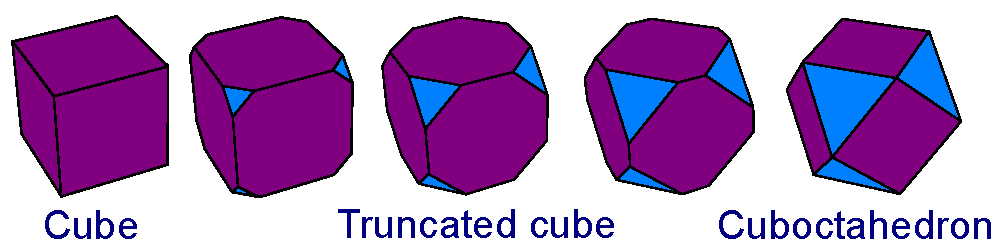
\includegraphics[width=1\textwidth]{../Resources/Figs/op_truncation.pdf}
        \caption{Trunctation and rectification operations visualised \cite{wikimedia-cube-truncation}}
        \label{fig:op_truncation}
    \end{figure}
    \item[Expansion/Cantellation] All the facets are pulled out away from the centroid of the polyhedron by the same distance without rescaling. The empty spaces are then filled with regular polygons in the following way: Edges that used to be identical in the original polyhedron are connected by adding a new a square. All the vertices that corresponded to a single vertex $v$ in the original polyhedron are connected by adding a $d$-gon where $d=deg(v)$.

    This operation can also be described as cantellation. The difference is in how we imagine the process that takes us to the resulting shape. From the viewpoint of cantellation, we first bevel (cut off) the edges and then apply truncation on what remained from the original vertices.
    \begin{figure}[H]
        \centering
        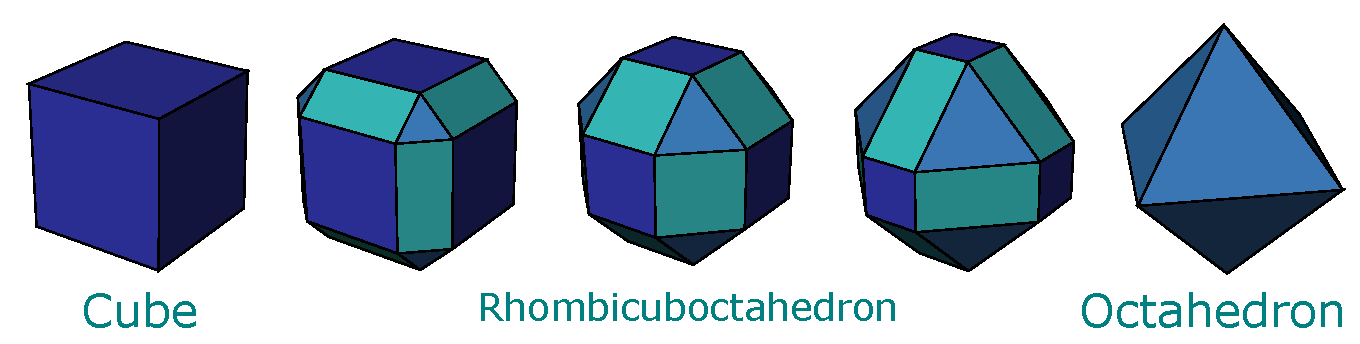
\includegraphics[width=1\textwidth]{../Resources/Figs/op_cantellation.pdf}
        \caption{Cantellation operation visualised \cite{wikimedia-cube-cantellation}}
        \label{fig:op_cantellation}
    \end{figure}
    \begin{highlight}
    \item[Snub] Is an application of expansion followed by splitting each new square in half in such a way, that we can twist the facets of the original Platonic solid.
    \end{highlight}
    \begin{figure}[H]
        \centering
        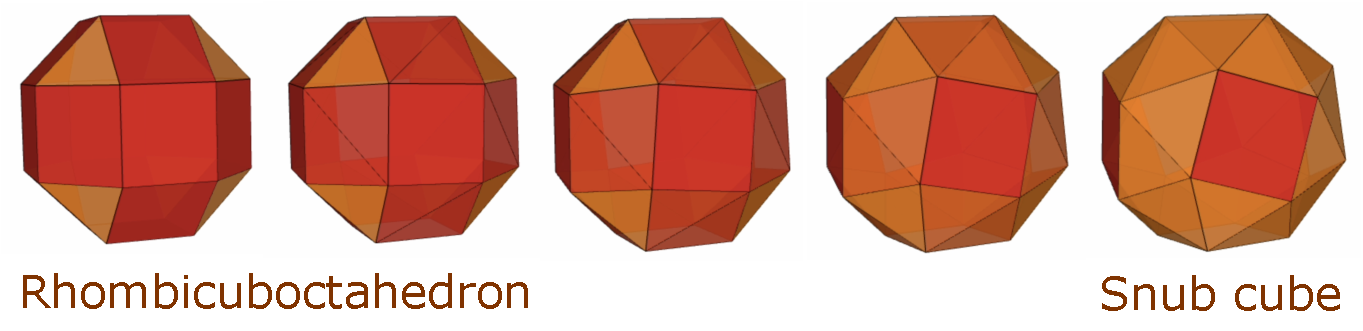
\includegraphics[width=1\textwidth]{../Resources/Figs/op_snub.pdf}
        \caption{Snub operation visualised \cite{natal-polyhed-viewer}}
        \label{fig:op_snub}
    \end{figure}
    
\end{description}

\section{Basic definitions and assumptions}

Here we state mathematical definitions, that should not be surprising in any way i.e. can be considered standard. Also, we state any assumptions we will make, which will then hold for the rest of this thesis.

\begin{definition}
    An \textit{undirected graph} $G$ is an ordered pair $G=(V,E)$ where $V$ is a set of vertices of the graph and $E \subseteq \binom{V}{2}$ is the set of its edges. 
\end{definition}

Since we are interested in Platonic and Archimedean solids, whose graphs are all planar, it is useful to define the notion of a \textit{plane graph}. This notion will correspond to a drawing of a particular graph onto a plane with one special property: the edges as they are drawn do not cross. 

\begin{highlight}
To avoid getting into too much detail, we will simply borrow the definition of a \textit{drawing} of a graph from the book \textit{Invitation to Discrete Mathematics} by Jaroslav Nešetřil and Jiří Matoušek \cite{matousek2009}.

\end{highlight}

A drawing of a graph might split the plane into multiple separate segments. We will call these segments \textit{faces} of a drawing of graph $G$.

\begin{definition}
    A graph $G$ is \textit{planar} if there exists a drawing of $G$ into a plane.
\end{definition}

\begin{definition}
    A \textit{plane graph} $G' = (V,E,F)$ is a drawing of a planar graph $G=(V,E)$ into plane where $F$ is the set of all faces of this drawing. We will also use the notation $V(G'), E(G'), F(G')$ to refer to sets $V,E,F$ respectively.
\end{definition}

In this thesis, we assume for any plane graph $G=(V,E,F)$ that the sets $V$, $E$ and $F$ are pairwise disjoint.


\section{Platonic and Archimedean graph properties}

\begin{highlight}
Here we would like to list some properties, that the graphs corresponding to the solids described above. Let $G=(V,E,F)$ be a plane graph of a solid with faces $F$. In the following tables $d$ is a number s.t. $\forall u \in V : \deg(u) = d$. The last column is a so called \textit{vertex configuration}, which denotes the amount of sides that the polygons incident with each vertex have. Note that the order of the numbers matters.
\end{highlight}

\begin{table}[H]
\centering
\begin{tabular}{l@{\hspace{1.5cm}}ccccc}
\toprule
\textbf{Platonic} & \textbf{$|V|$} & \textbf{$|E|$} & \textbf{$|F|$} & \textbf{$d$} & \textbf{Vertex config.} \\
\midrule
cube & 8 & 12 & 6 & 3 & 4.4.4 \\
dodecahedron & 20 & 30 & 12 & 3 & 5.5.5 \\
icosahedron & 12 & 30 & 20 & 5 & 3.3.3.3.3 \\
octahedron & 6 & 12 & 8 & 4 & 3.3.3.3 \\
tetrahedron & 4 & 6 & 4 & 3 & 3.3.3 \\
\bottomrule
\end{tabular}
\caption{Basic properties of Platonic graphs}
\label{tab:platonic-basic-props}
\end{table}

\begin{table}[H]
\centering
\begin{tabular}{l@{\hspace{1.5cm}}ccccc}
\toprule
\textbf{Archimedean} & \textbf{$|V|$} & \textbf{$|E|$} & \textbf{$|F|$} & \textbf{$d$} & \textbf{Vertex config.} \\
\midrule
cuboctahedron & 12 & 24 & 14 & 4 & 3.4.3.4 \\
icosidodecahedron & 30 & 60 & 32 & 4 & 3.5.3.5 \\
rhombicosidodecahedron & 60 & 120 & 62 & 4 & 3.4.5.4 \\
rhombicuboctahedron & 24 & 48 & 26 & 4 & 3.4.4.4 \\
snub cube & 24 & 60 & 38 & 5 & 3.3.3.3.4 \\
snub dodecahedron & 60 & 150 & 92 & 5 & 3.3.3.3.5 \\
truncated cube & 24 & 36 & 14 & 3 & 3.8.8 \\
truncated cuboctahedron & 48 & 72 & 26 & 3 & 4.6.8 \\
truncated dodecahedron & 60 & 90 & 32 & 3 & 3.10.10 \\
truncated icosahedron & 60 & 90 & 32 & 3 & 5.6.6 \\
truncated icosidodecahedron & 120 & 180 & 62 & 3 & 4.6.10 \\
truncated octahedron & 24 & 36 & 14 & 3 & 4.6.6 \\
truncated tetrahedron & 12 & 18 & 8 & 3 & 3.6.6 \\
\bottomrule
\end{tabular}
\caption{Basic properties of Archimedean graphs}
\label{tab:archimedean-basic-props}
\end{table}
\chapter{Defining colorings}

\section{The general concept of coloring}

As we will be working with many types of colorings, we introduce a general notion of an abstract coloring, which all specific types will share, in order to avoid repetition.

\begin{defn}[partial function]
    A \emph{partial function} is a function $f : X \rightarrow Y$ such that for all $x \in X$, either $f(x) \in Y$ or $f(x)$ is undefined.
\end{defn}

Since we are concerned with graphs of Platonic and Archimedean solids—which are all planar—we define the concept of coloring directly on their plane graphs, i.e., as they are drawn in the plane, rather than considering their abstract representations.

\begin{defn}[coloring]
    Let $S$ be a set, and let $G = (V, E, F)$ be a plane graph. We define a \emph{coloring} of $G$ as a partial function $c : V \cup E \cup F \rightarrow S$ together with a coloring rule $R$ that restricts which elements of the graph may be assigned the same color, i.e., mapped to the same element of $S$.
\end{defn}

In other words, a coloring is an assignment of elements in $S$ to vertices, edges, or faces of some plane graph. We can think of elements of $S$ as colors, but usually we will use numbers instead. What is especially important to us is whether any two elements are mapped onto the same target, i.e., colored by the same color. The coloring rule then prevents some assignments from being considered valid. This makes the coloring problem non-trivial.

\begin{defn}[family of colorings]
    For a graph $G$, let the set of all colorings of $G$ sharing the same coloring rule $R$ be called a \emph{family of colorings} of $G$.
\end{defn}

\begin{defn}[$k$-coloring]
    Let $G = (V, E, F)$ be a plane graph. Let $C$ be a family of colorings of $G$. Let $S$ be a set such that $|S| = k$ for some $k \in \mathbb{N}$. A function $c \in C$ such that $c : V \cup E \cup F \rightarrow S$ is called a \emph{$k$-coloring} of $G$.
\end{defn}

Note that a $k$-coloring does not necessarily use all of the $k$ available colors. Mathematically speaking, a $k$-coloring is not necessarily a surjective function.

\begin{defn}[$k$-colorable graph]
    For a plane graph $G$, a family of colorings $C$, and a natural number $k$, if there exists a $k$-coloring of $G$, then we say that $G$ is \emph{$k$-colorable}.
\end{defn}

A typical question we ask when considering colorings of a graph is: What is the smallest number of colors we can use to color the graph without violating the coloring rule? This leads to the definition of the so-called \textit{chromatic number}.


\begin{defn}[chromatic number]
    For a plane graph $G$ and a family of colorings $C$, the \emph{chromatic number} $\chi^C(G)$ is the minimum $k \in \mathbb{N}$ such that $G$ is $k$-colorable.
\end{defn}

Once we know a graph is $k$-colorable, there is another interesting property of the graph we can examine. We can ask about how many different colorings with $k$ colors there exists for the given graph. A closely related concept to this question is the \emph{chromatic polynomial}. But first, we need to define when two colorings are considered different.

\begin{defn}[different colorings]
    Given a plane graph $G = (V, E, F)$, a family of colorings $C$, and $k$-colorings $c_1, c_2 \in C$, we say $c_1$ and $c_2$ are \emph{different} if there exists $x \in V \cup E \cup F$ such that $c_1(x) \neq c_2(x)$.
\end{defn}

The definition above states that if two colorings assign different colors to any element, then the colorings are considered different. Note that this does not take into account any symmetries of the graph.

\begin{defn}[chromatic polynomial]
    For a graph $G$ and a family of colorings $C$, the \emph{chromatic polynomial}, denoted by $P_C(G,x)$ is a function such that for all $k \in \mathbb{N}$, we have $P_C(G,k) = n$, where $n$ is the number of different $k$-colorings of $G$.
\end{defn}

\section{Particular types of colorings}

\subsection{Vertex coloring}

\begin{defn}[vertex coloring]
    Given a set $S$ a \emph{vertex coloring} of a plane graph $G = (V, E, F)$ is any coloring $c : V \rightarrow S$ belonging to family of colorings with the following coloring rule:
    \begin{equation}\label{eqn:vtx_rule}
        \forall u, v \in V, \quad \text{if } \{u, v\} \in E, \text{ then } c(u) \neq c(v). 
        \tag{$R_V$}
    \end{equation}
    We denote this family of colorings by $X$.
\end{defn}

In other words, a vertex coloring is an assignment of colors to each vertex such that no two adjacent vertices share the same color.

\begin{figure}[H]
    \centering
    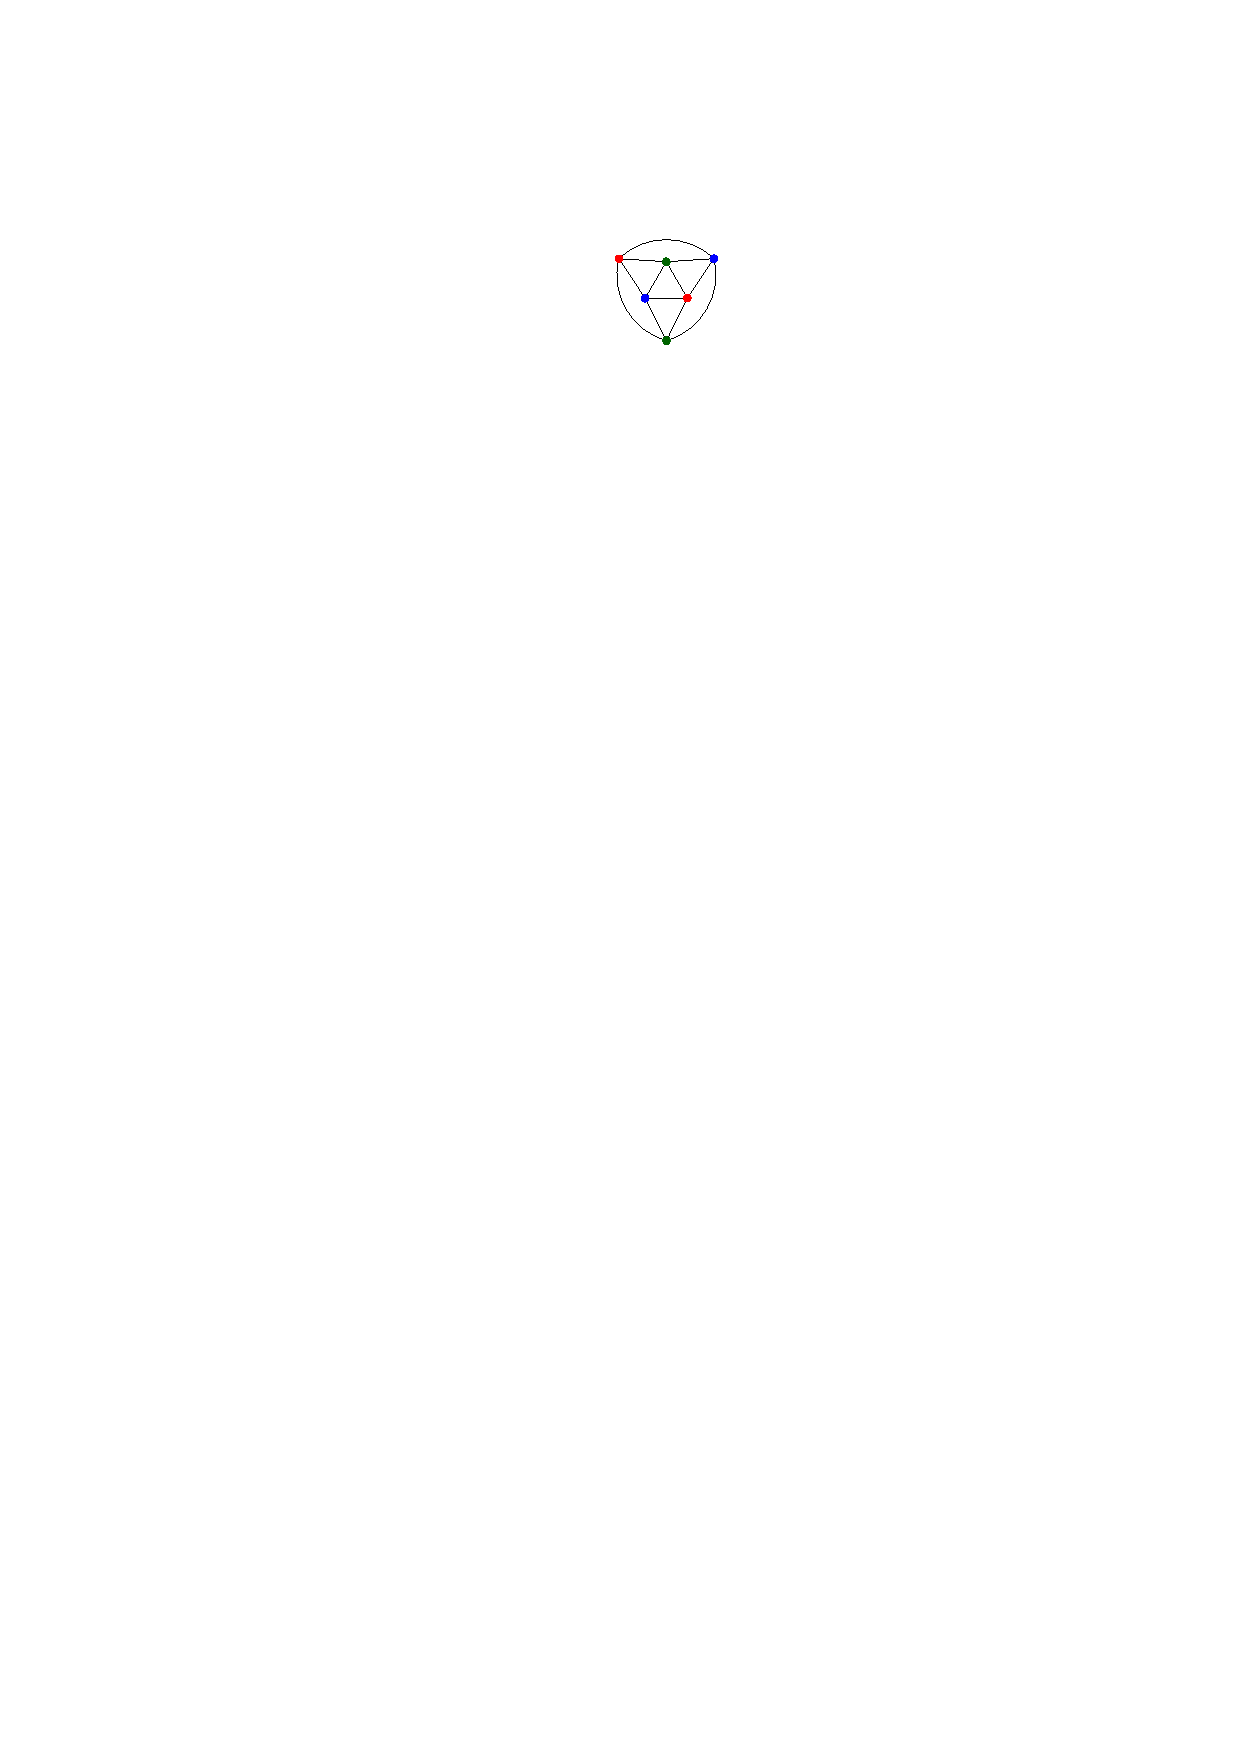
\includegraphics[width=0.20\textwidth]{../Resources/Figs/octahedral_vtx_colr.pdf}
    \caption{Vertex coloring of the octahedral graph}
    \label{fig:octahedral_vtx_coloring}
\end{figure}

The graph in Figure~\ref{fig:octahedral_vtx_coloring} has vertex chromatic number 3.

\subsection{Edge coloring}

\begin{defn}[edge coloring]
    Let $S$ be a set. An \emph{edge coloring} of a plane graph $G = (V, E, F)$ is a coloring $c : E \rightarrow S$ belonging to a family of colorings with the following rule: 
    \begin{equation}\label{eqn:edge_rule}
     \forall e, f \in E, \quad \text{ if } e \cap f \neq \emptyset, \text{ then } c(e) \neq c(f). \tag{$R_E$}
    \end{equation}
    We denote this family of colorings by $X'$.
   
\end{defn}

This rule states that any two edges sharing a common endpoint must be assigned different colors.

\begin{figure}[H]
    \centering
    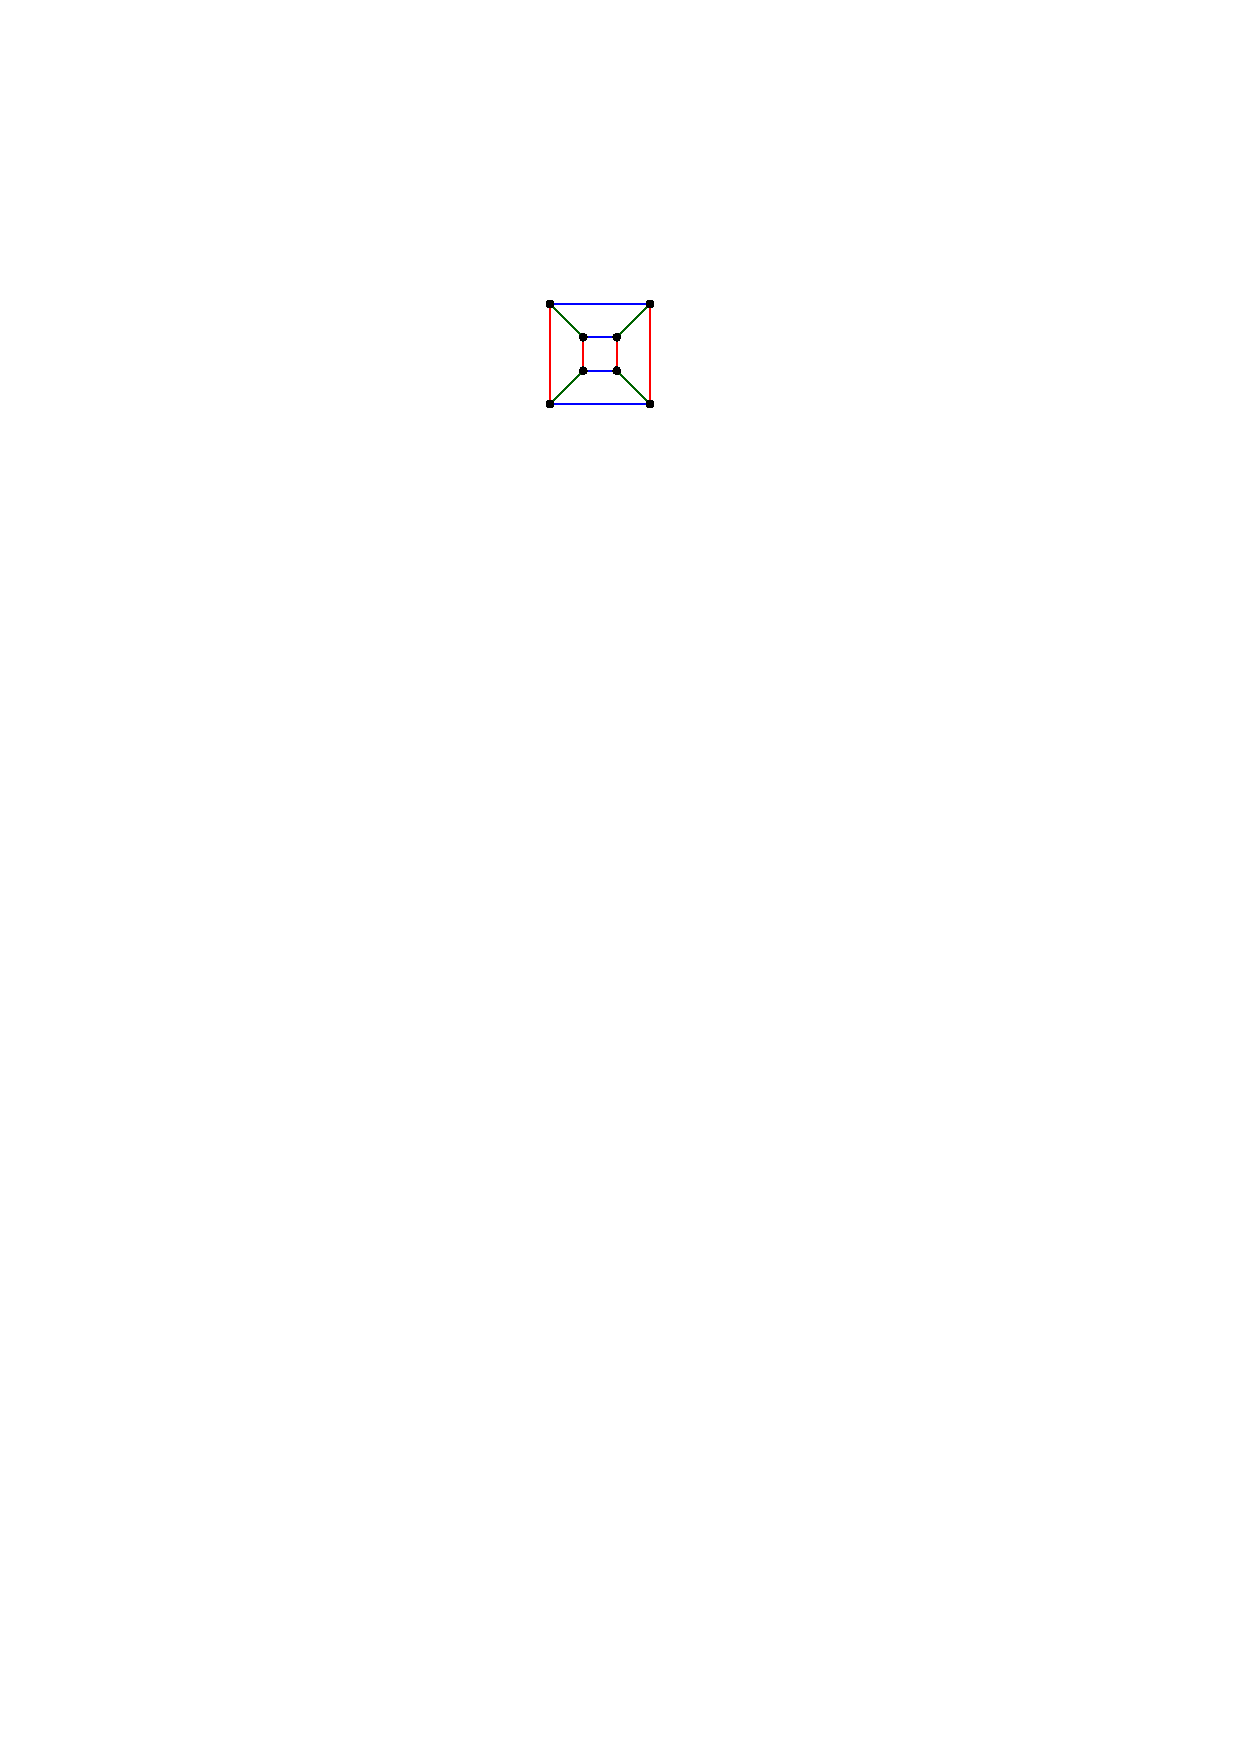
\includegraphics[width=0.2\textwidth]{../Resources/Figs/cubical_edg_colr.pdf}
    \caption{Edge coloring of the cubical graph}
    \label{fig:cubical_edge_coloring}
\end{figure}



\subsection{Total coloring}

By combining vertex and edge colorings and adding one additional constraint, we obtain the so-called \textit{total coloring} \cite{behzad65}.

\begin{defn}[total coloring]
    Given a set $S$ a \emph{total coloring} of a plane graph $G = (V, E, F)$ is a coloring $c : V \cup E \rightarrow S$ from a family of colorings sharing both coloring rules \ref{eqn:vtx_rule} and \ref{eqn:edge_rule}, as well as the following additional rule:
    \begin{equation}\label{eqn:tot_rule}
    \forall v \in V, \ \forall e \in E, \ \text{if } v \in e, \text{ then } c(v) \neq c(e). \tag{$R_T$}
    \end{equation}
    We denote this family of colorings by $X''$.
\end{defn}

\begin{figure}[H]
    \centering
    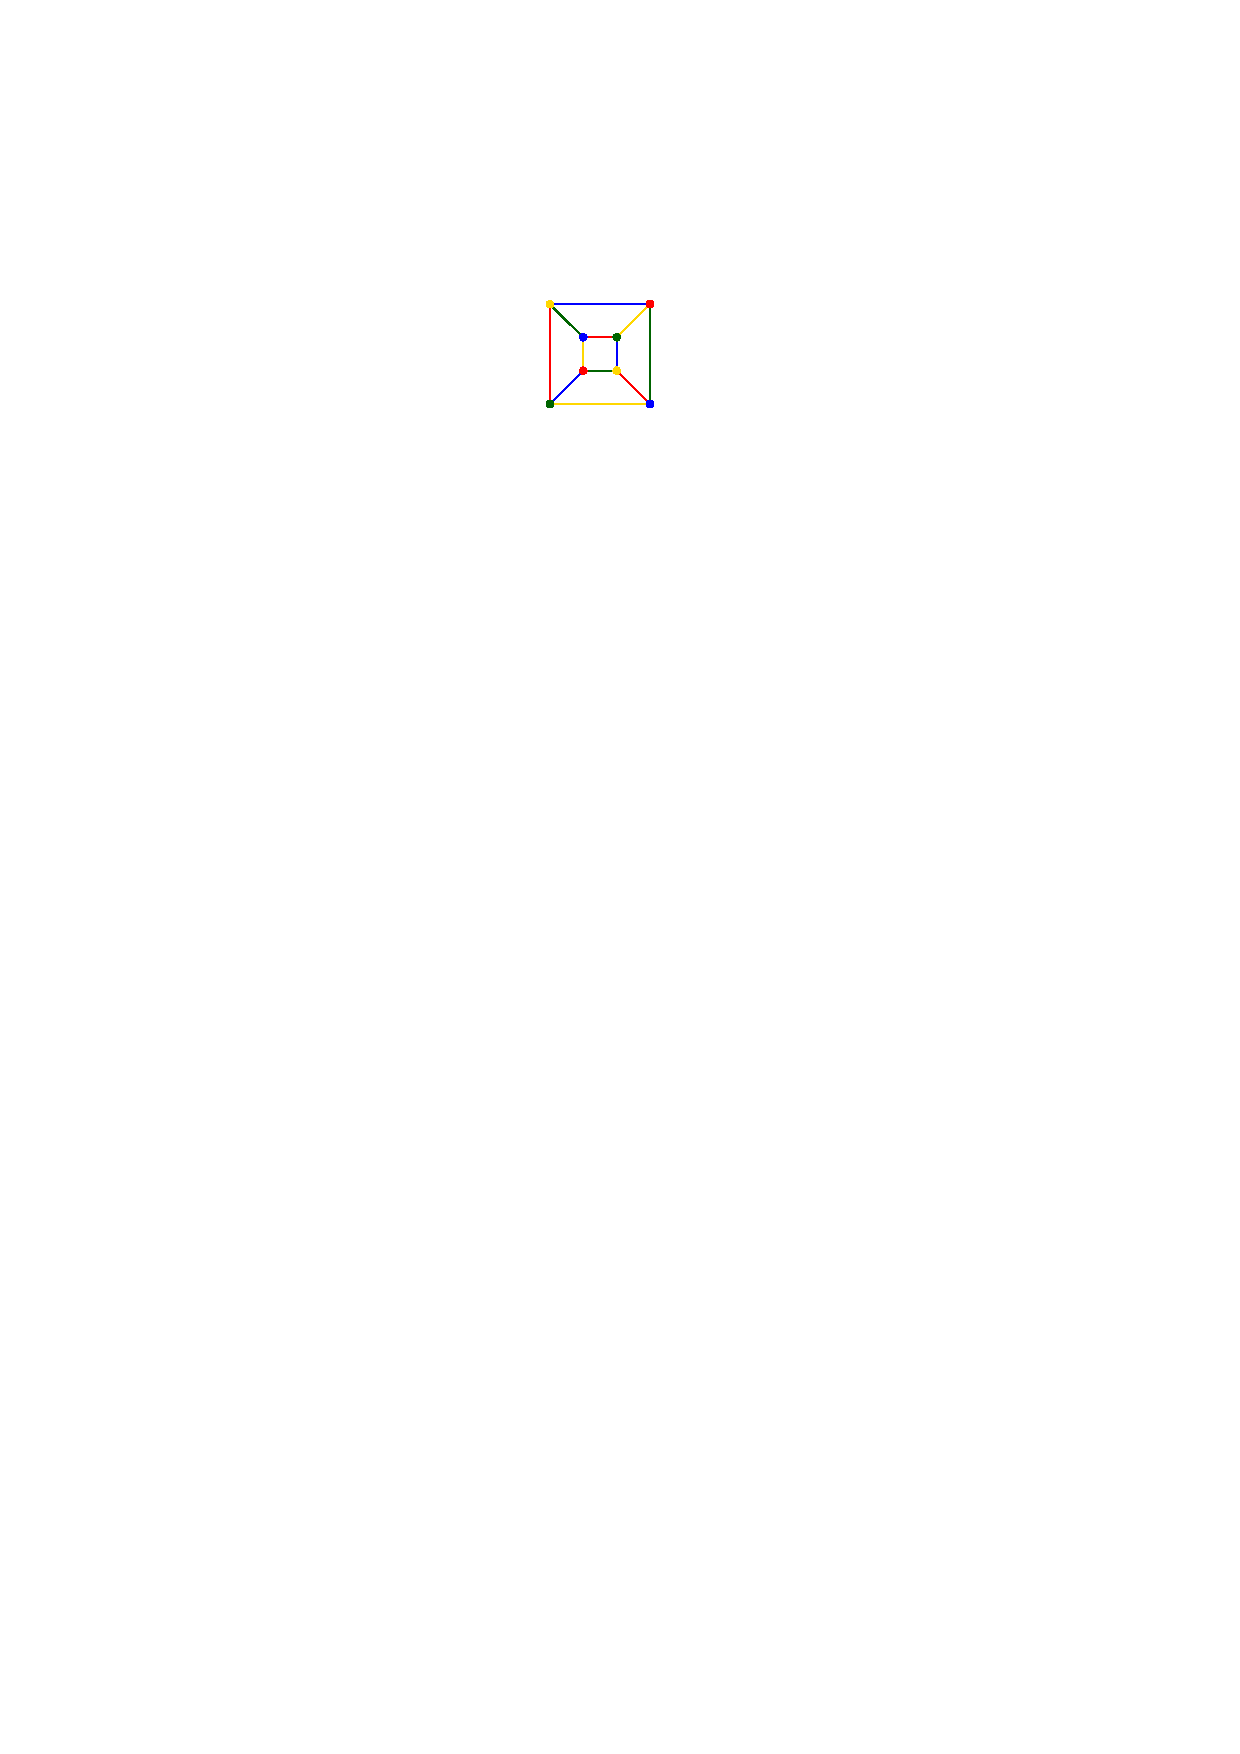
\includegraphics[width=0.2\textwidth]{../Resources/Figs/cubical_tot_colr_opt.pdf}
    \caption{Total coloring of the cubical graph using four colors}
    \label{fig:cubical_tot_coloring}
\end{figure}

\begin{figure}[H]
    \centering
    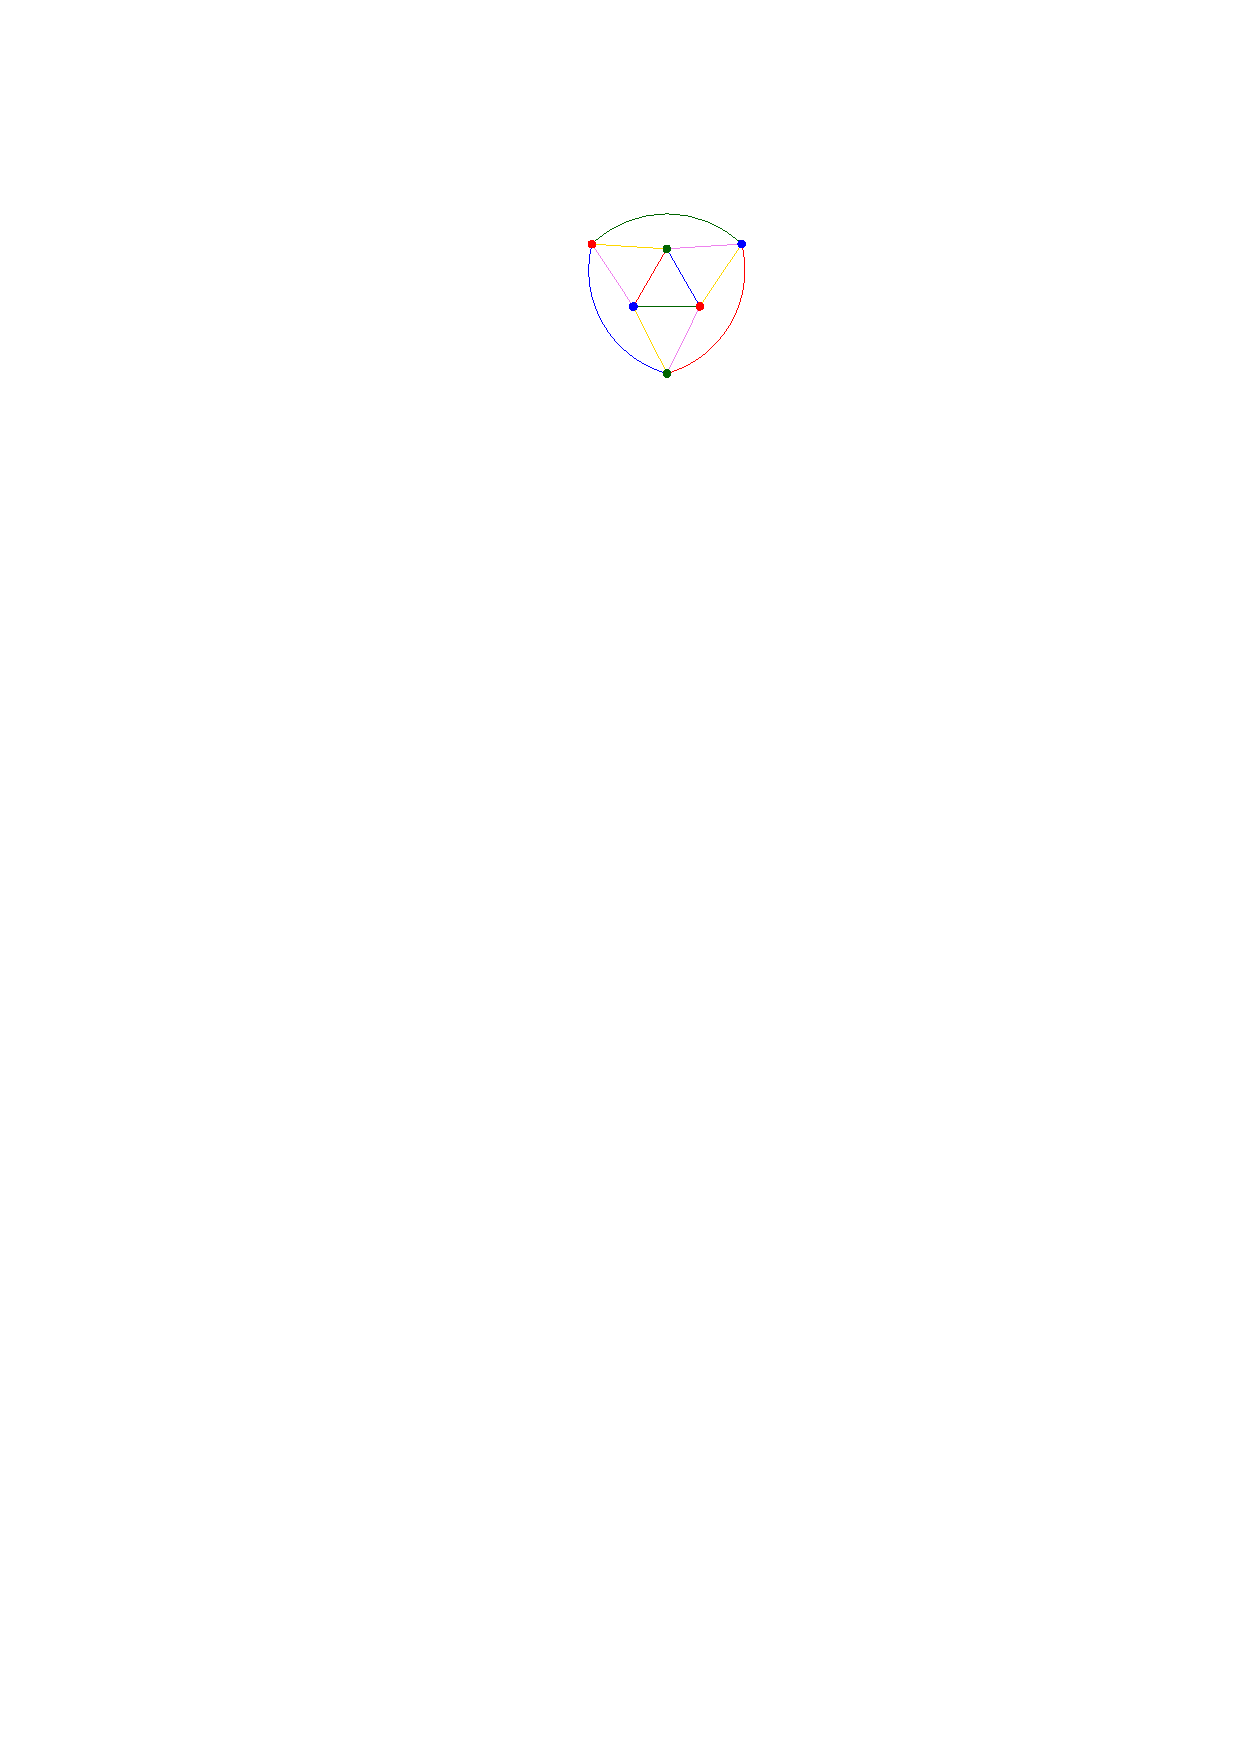
\includegraphics[width=0.25\textwidth]{../Resources/Figs/octahedral_tot_colr.pdf}
    \caption{Total coloring of the octahedral graph using five colors}
    \label{fig:octahedral_tot_coloring}
\end{figure}

\subsection{Face coloring}

Since we consider planar graphs, we can also color the faces of the corresponding plane graphs.

\begin{defn}[boundary]
    For a plane graph $G=(V,E,F)$ and a face $R \in F$, we define the \emph{boundary} of $R$, denoted by $\bnd(R)$, as the set of all edges incident with $R$.
\end{defn}

\begin{defn}[face coloring]
    Given a set $S$ and a plane graph $G = (V, E, F)$, a \emph{face coloring} is any function $c : F \rightarrow S$ belonging to a family of colorings with the following coloring rule:
    \begin{equation}\label{eqn:face_rule}
     \forall R_1, R_2 \in F, \ \text{if } \bnd(R_1) \cap \bnd(R_2) \neq \emptyset, \text{ then } c(R_1) \neq c(R_2). \tag{$R_F$}
    \end{equation}
    We denote this family of colorings by $X^F$.
\end{defn}

\begin{figure}[H]
    \centering
    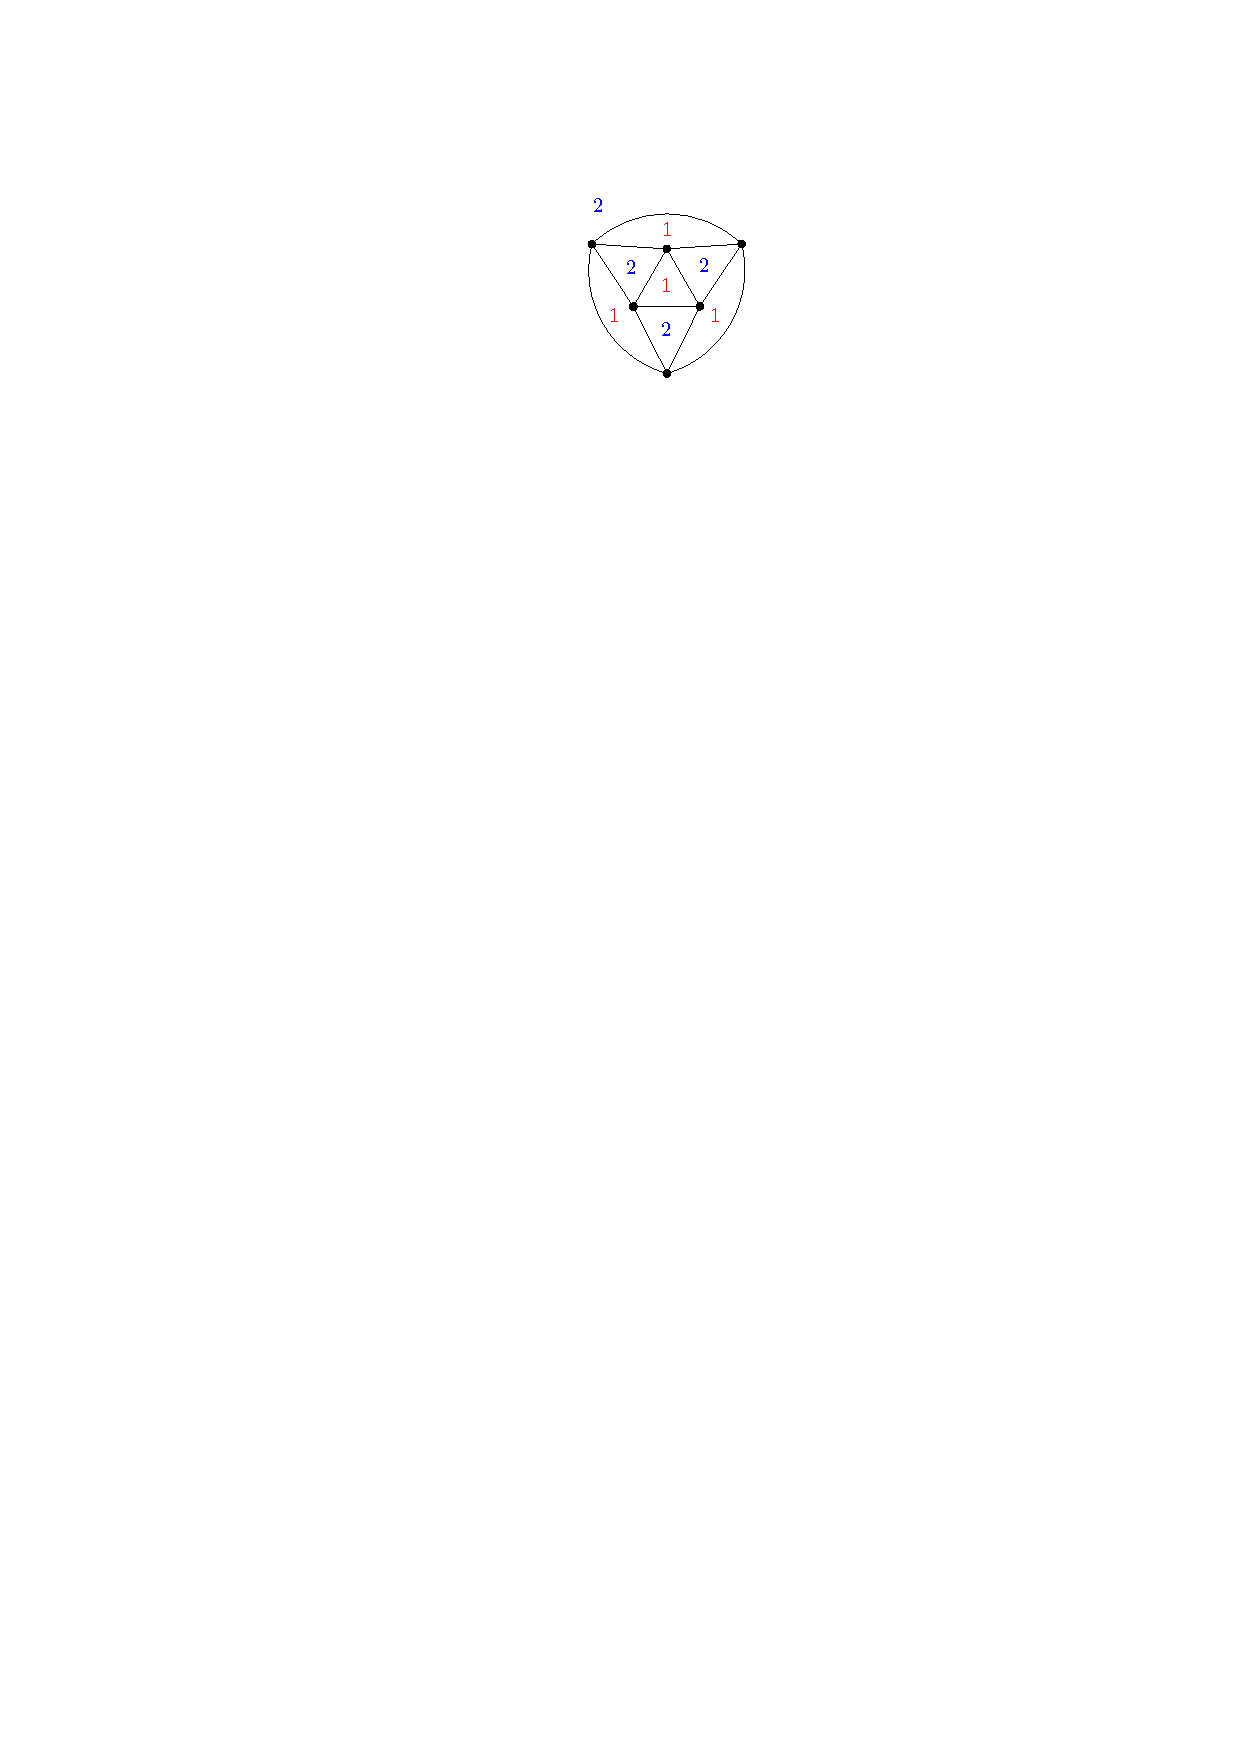
\includegraphics[width=0.2\textwidth]{../Resources/Figs/octahedral_face_colr.pdf}
    \caption{Face coloring of the octahedral graph using two colors (1 and 2)}
    \label{fig:face_tot_coloring}
\end{figure}

\subsection{Rainbow coloring}

So far, the particular colorings we have considered were all quite similar to each other. In what sense? All of their coloring rules were based on the notion of adjacency of some elements, i.e., neighboring vertices, incident edges etc. could not share the same color. There exist other types of colorings, where the coloring rules are based on other concepts, such as connectivity. One such example is the \textit{rainbow coloring} \cite{chartrand08}.

\begin{defn}[rainbow coloring]
    Let $S$ be a set. A \emph{rainbow coloring} of a plane graph $G = (V, E, F)$ is a coloring $c : E \rightarrow S$ belonging to a family of colorings with the following rule: 
    \begin{equation}\label{eqn:rainbow_rule}
     \forall u, v \in V, \ \exists uv \text{-path } (u, e_1, w_1, \ldots , w_{n-1}, e_n, v) \text{ s.t. } \forall i \neq j : c(e_i) \neq c(e_j). \tag{$R_R$}
    \end{equation}
    We denote this family of colorings by $X^R$.
\end{defn}

\begin{figure}[H]
    \centering
    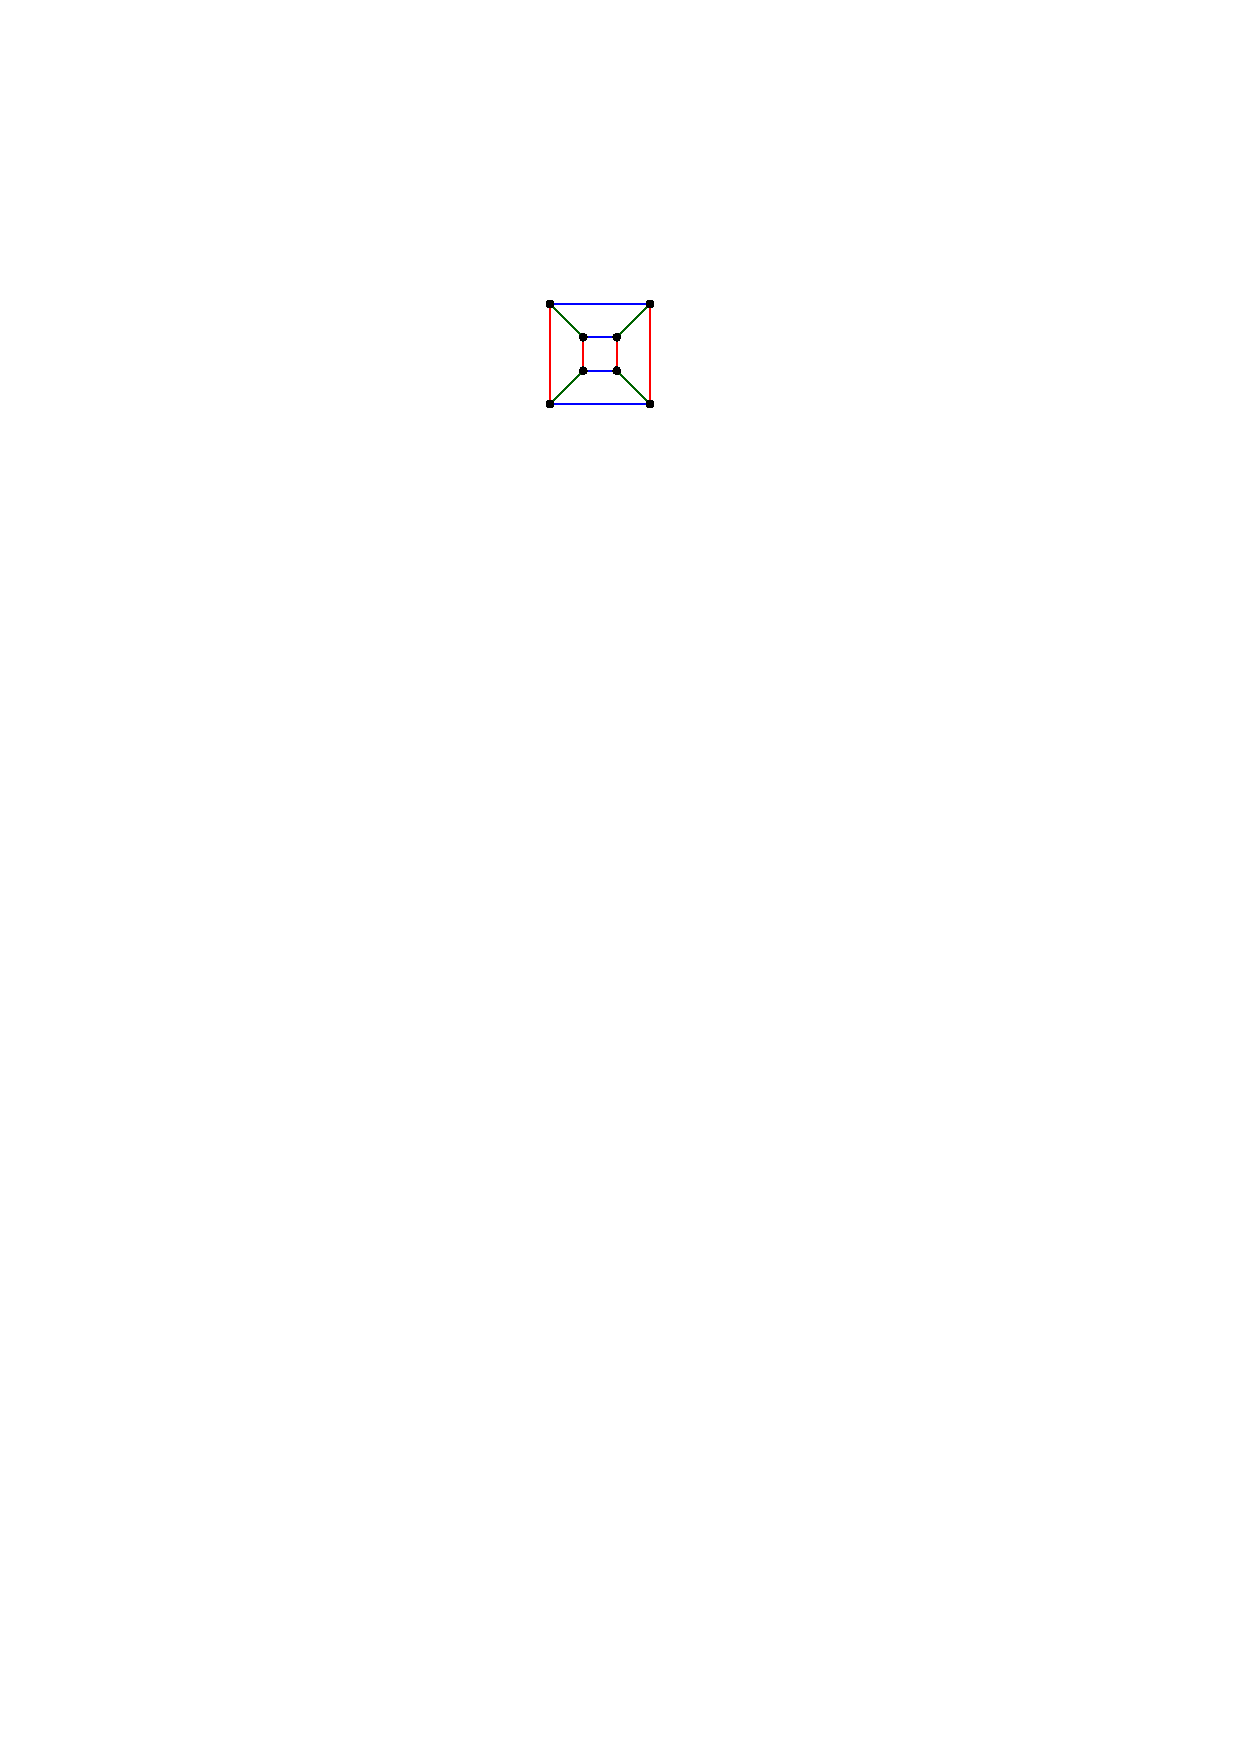
\includegraphics[width=0.2\textwidth]{../Resources/Figs/cubical_edg_colr.pdf}
    \caption{Rainbow coloring of the cubical graph. Let us appreciate the fact that it is also a proper edge coloring.}
    \label{fig:cubical_rainbow_coloring}
\end{figure}

\begin{figure}[H]
    \centering
    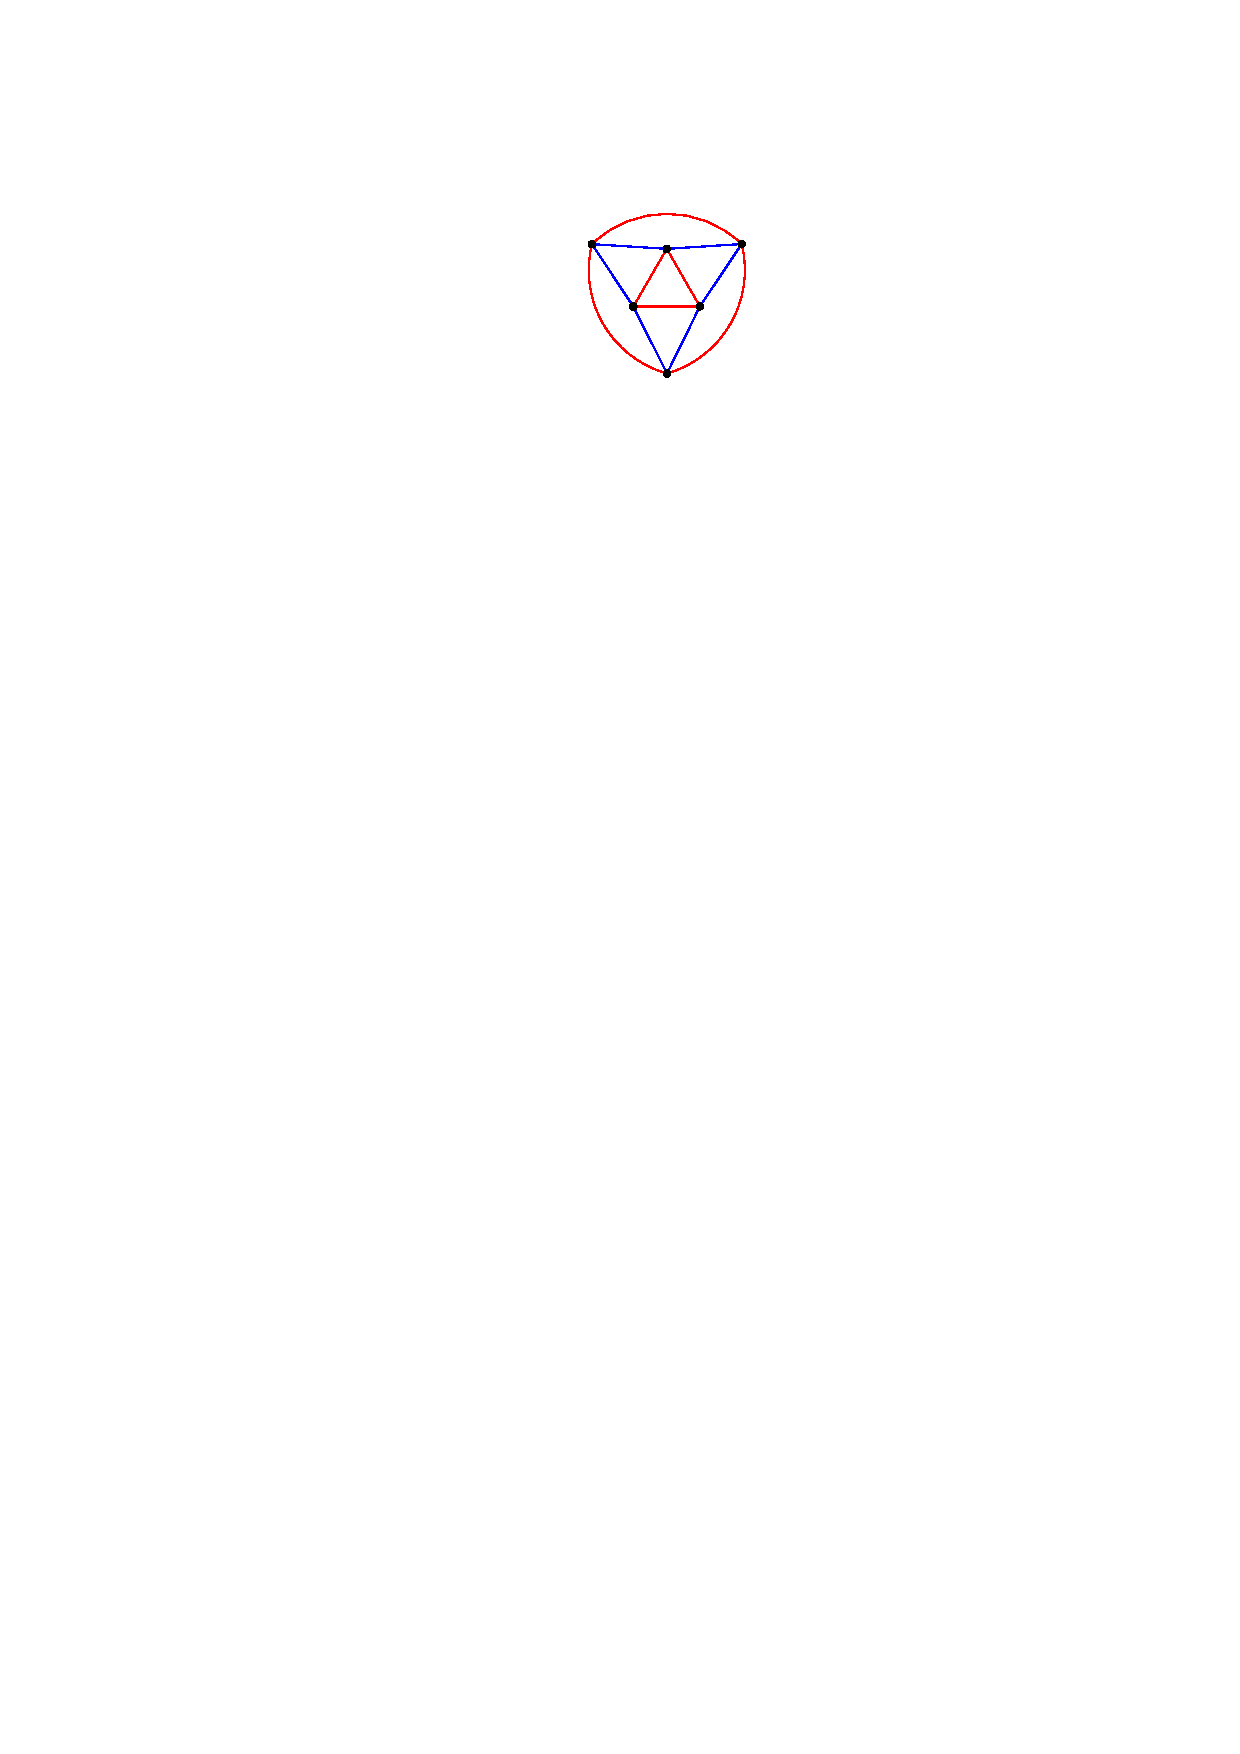
\includegraphics[width=0.25\textwidth]{../Resources/Figs/octahedral_rainbow_colr.pdf}
    \caption{Rainbow coloring of octahedral graph. Note that it is not a proper edge coloring.}
    \label{fig:octahedral_rainbow_coloring}
\end{figure}

\subsection{Magic labeling}

There also exist coloring rules that depend on the actual values of the colors. In such cases, the colors must come from a subset of the natural numbers, where arithmetic operations (such as addition) are defined. These colorings are usually referred to as \textit{labelings}.

All labelings share the notion of assigning a \textit{weight} to the elements of a graph. For an element $x$, we denote its weight by $w(x)$. Using this notation, we define an \textit{edge labeling} as a function $l : E \rightarrow \mathbb{N}$ and analogously, a \textit{vertex labeling} as a function $l : V \rightarrow \mathbb{N}$

Moreover, we call an edge labeling \textit{magic} if there exists $k \in \mathbb{N}$ such that $\forall v \in V: w(v) = k$, where $w$ is a weight function defined in terms of $l$. In other words, an edge labeling $l$ is magic if all vertices have the same weight when edges are labeled using $l$. For example, we might define $w(v) = \sum_{uv \in E} l(uv)$. An analogous definition holds for magic vertex labeling.

All labeling definitions above are based on the book \textit{Magic Graphs} by Wallis \cite{marrwall2013}.
\chapter{Connections between colorings}
\label{chap:clring_conversions}
 
Many times, we can reduce a particular mathematical problem to another one that is less complex or has been studied for a longer time. In this way, we can also reduce some of the specific coloring problems to vertex coloring problems, which are the most extensively researched of them all.

In our case, it is useful that there exists a wide range of algorithms and known results for vertex coloring, which we can leverage when working with less traditional coloring types.

Note that the conversions themselves are not novel and are also well known.

\section{Edge coloring to vertex coloring}

\begin{defn}[line graph]
    For a graph $G = (V, E)$, we define the \emph{line graph} $G_L = (V_L, E_L)$ as follows:
    \begin{enumerate}
        \item $V_L := E$
        \item $E_L := \{ \{e, f\} \in \binom{E}{2} : e \cap f \neq \emptyset \}$
    \end{enumerate}
\end{defn}

In other words, the vertices of the line graph are exactly the edges of the original graph. Two vertices in the line graph are connected if and only if their corresponding edges in the original graph share a common endpoint. Notice how the defining property of the set $E_L$ coincides with the coloring rule for edge coloring \ref{eqn:edge_rule}.

\begin{figure}[H]
    \centering
    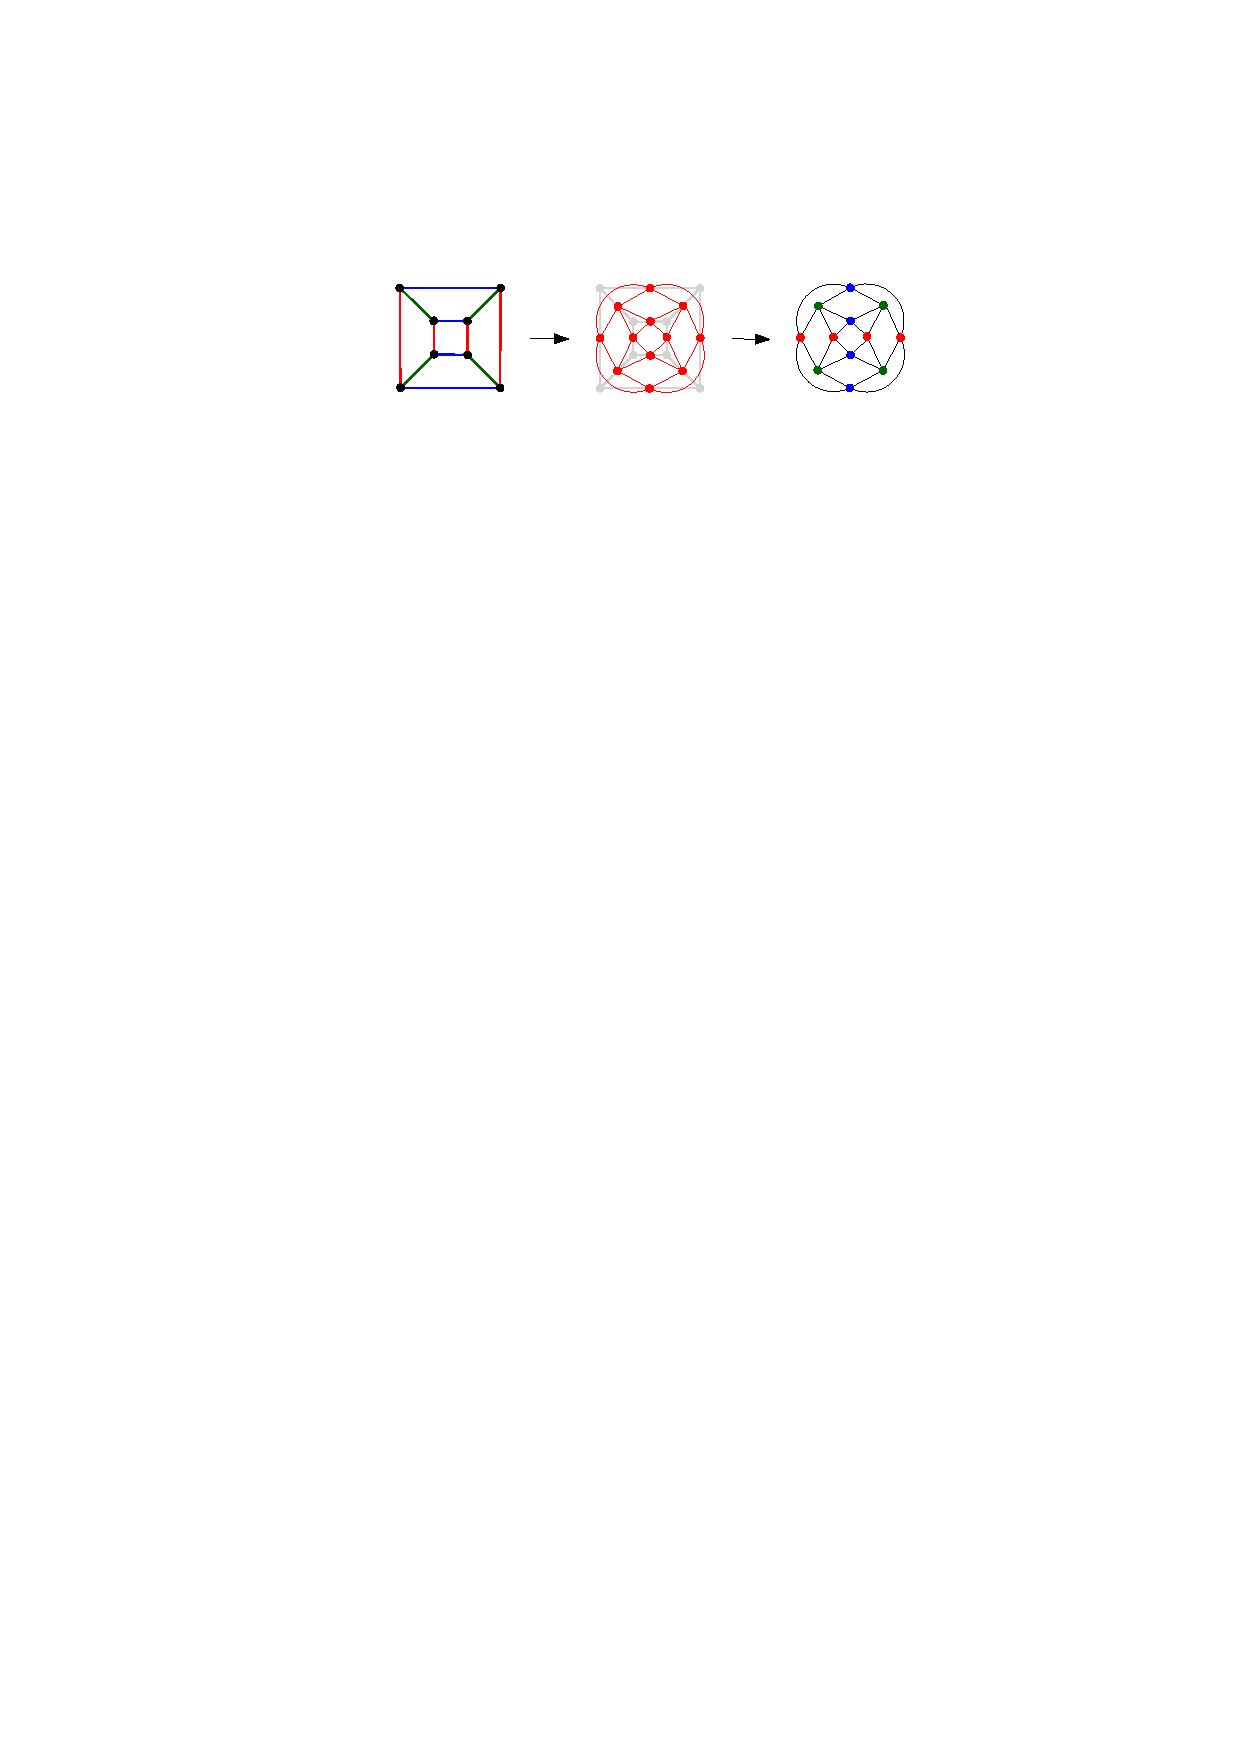
\includegraphics[width=1\textwidth]{../Resources/Figs/cubical_line_graph.pdf}
    \caption{Visualization of conversion from edge coloring to vertex coloring using a line graph}
    \label{fig:cubical_line_graph}
\end{figure}

Note that in Figure~\ref{fig:cubical_line_graph} above, the operation of creating the line graph corresponds to the cube rectification operation. In this particular case, we transformed the graph of a cube into the graph of a cuboctahedron.

\section{Total coloring to vertex coloring}

Intuitively, since total coloring assigns colors to both edges and vertices, it makes sense to use a combination of the original graph and its line graph. However, we cannot simply combine these two graphs by taking the union of their vertex and edge sets and then apply vertex coloring to the resulting graph. The problem is that nothing would prevent us from assigning the same color to an edge and one of its endpoints, since the vertices corresponding to the edge and its endpoint would not be adjacent in the combined graph. This brings us to the so-called \textit{incidence graph}.

\begin{defn}[incidence graph]
    For a graph $G = (V, E)$, we define its \emph{incidence graph} $G_I = (V_I, E_I)$ as follows:
    \begin{enumerate}
        \item $V_I := V \cup E$
        \item $E_I := \{ \{v, e\} : v \in V, e \in E, v \in e \}$
    \end{enumerate}
\end{defn}

Again, note how the definition of $E_I$ corresponds to the coloring rule \ref{eqn:tot_rule}.

\begin{figure}[H]
    \centering
    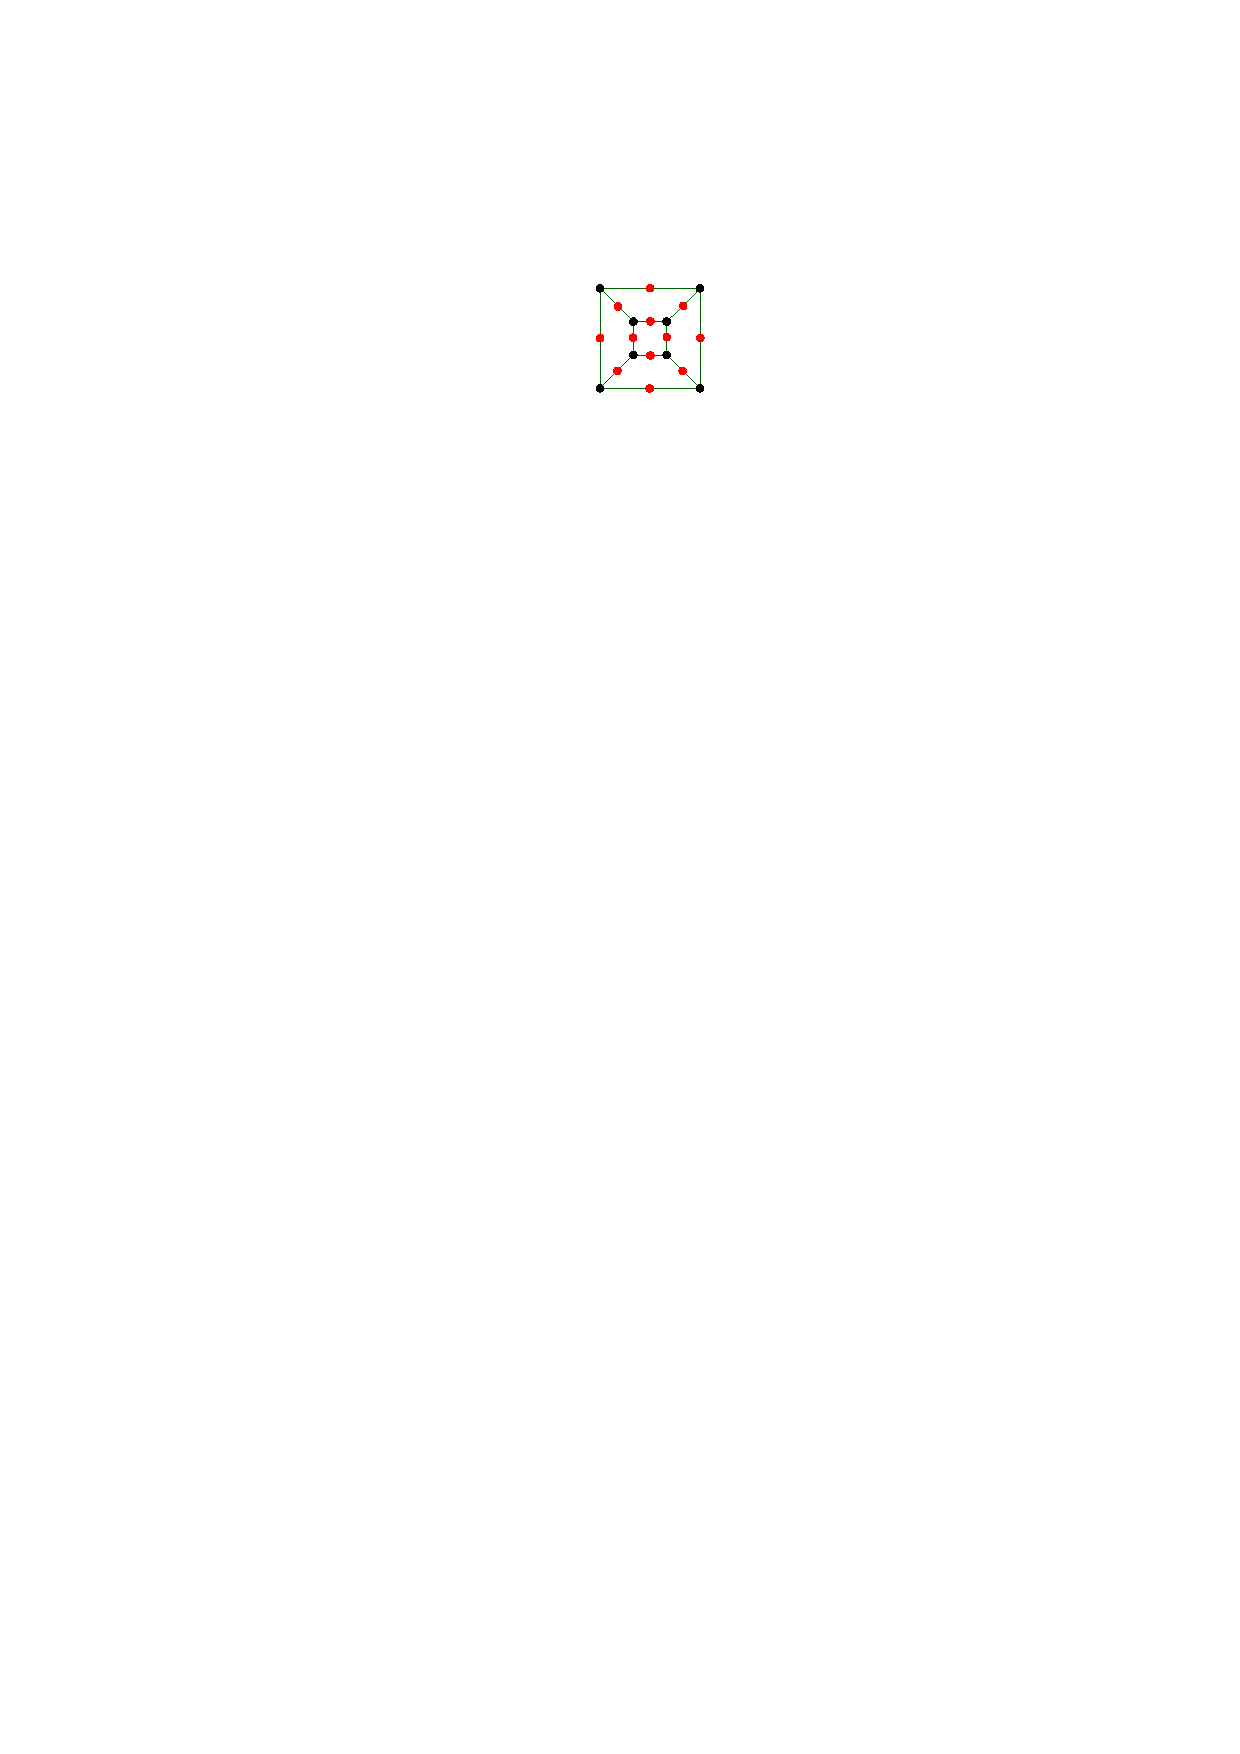
\includegraphics[width=0.2\textwidth]{../Resources/Figs/cubical_incid_graph.pdf}
    \caption{Example of the incidence graph of a cubical graph}
    \label{fig:cubical_incid_graph}
\end{figure}

Now we have all the necessary tools to define a \textit{total graph}, which has the property that its vertex coloring corresponds exactly to the total coloring of the original graph.

\begin{defn}[total graph]
    Let $G = (V, E)$ be a graph. Let $G_L = (V_L, E_L)$ and $G_I = (V_I, E_I)$ be its line graph and incidence graphs, respectively. We define its \emph{total graph} $G_T = (V_T, E_T)$ as follows:
    \begin{enumerate}
        \item $V_T := V_I$
        \item $E_T := E \cup E_L \cup E_I$
    \end{enumerate}
\end{defn}

In natural language, we start with the vertices and edges of the incidence graph. Then, we split the vertices of the incidence graph into two disjoint sets: the set of vertices of the original graph and the set of vertices of the line graph. In the former set, we connect any two vertices that are adjacent in the original graph. In the latter case, we do the same using adjacency in the line graph.

\begin{figure}[H]
    \centering
    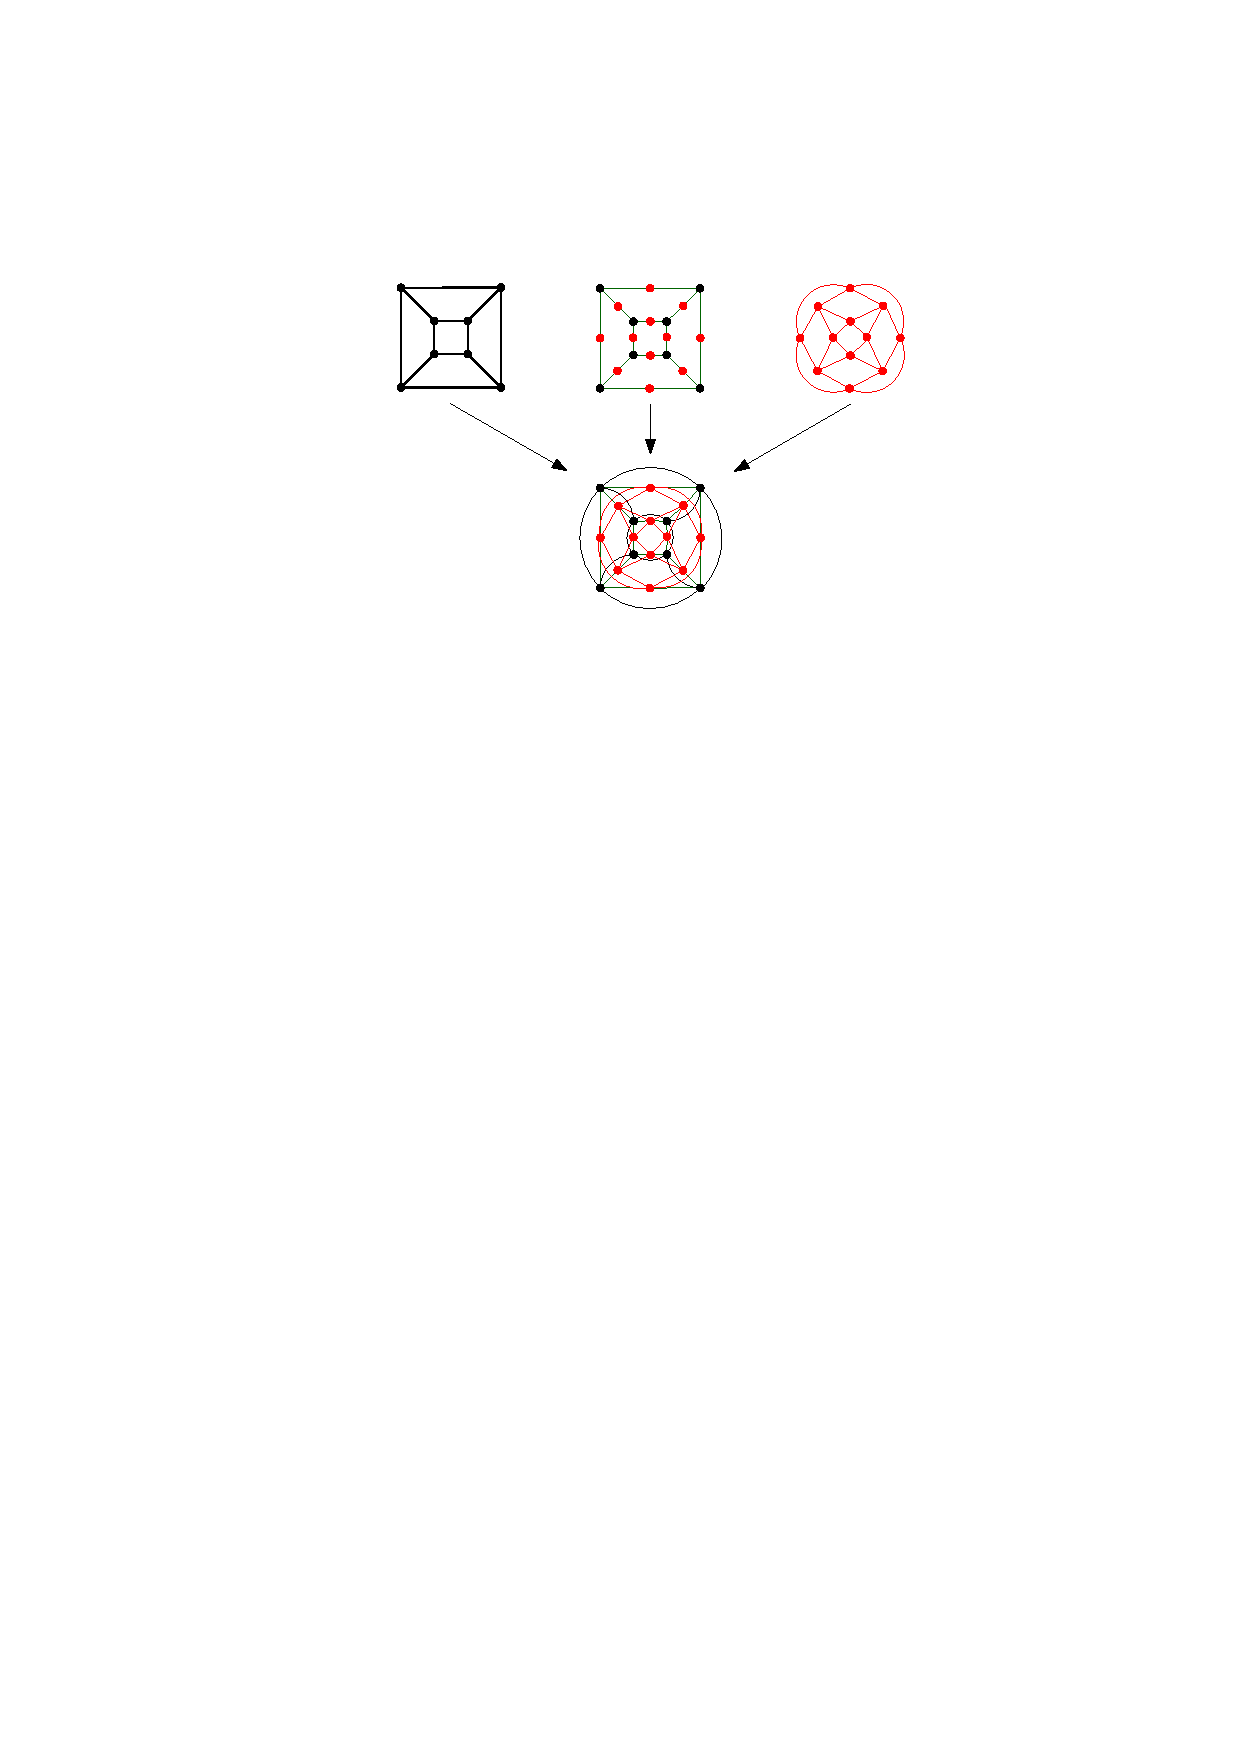
\includegraphics[width=1\textwidth]{../Resources/Figs/cubical_total_graph.pdf}
    \caption{Visualization of total graph construction from the original graph, incidence graph, and line graph.}
    \label{fig:cubical_total_graph}
\end{figure}

\begin{figure}[H]
    \centering
    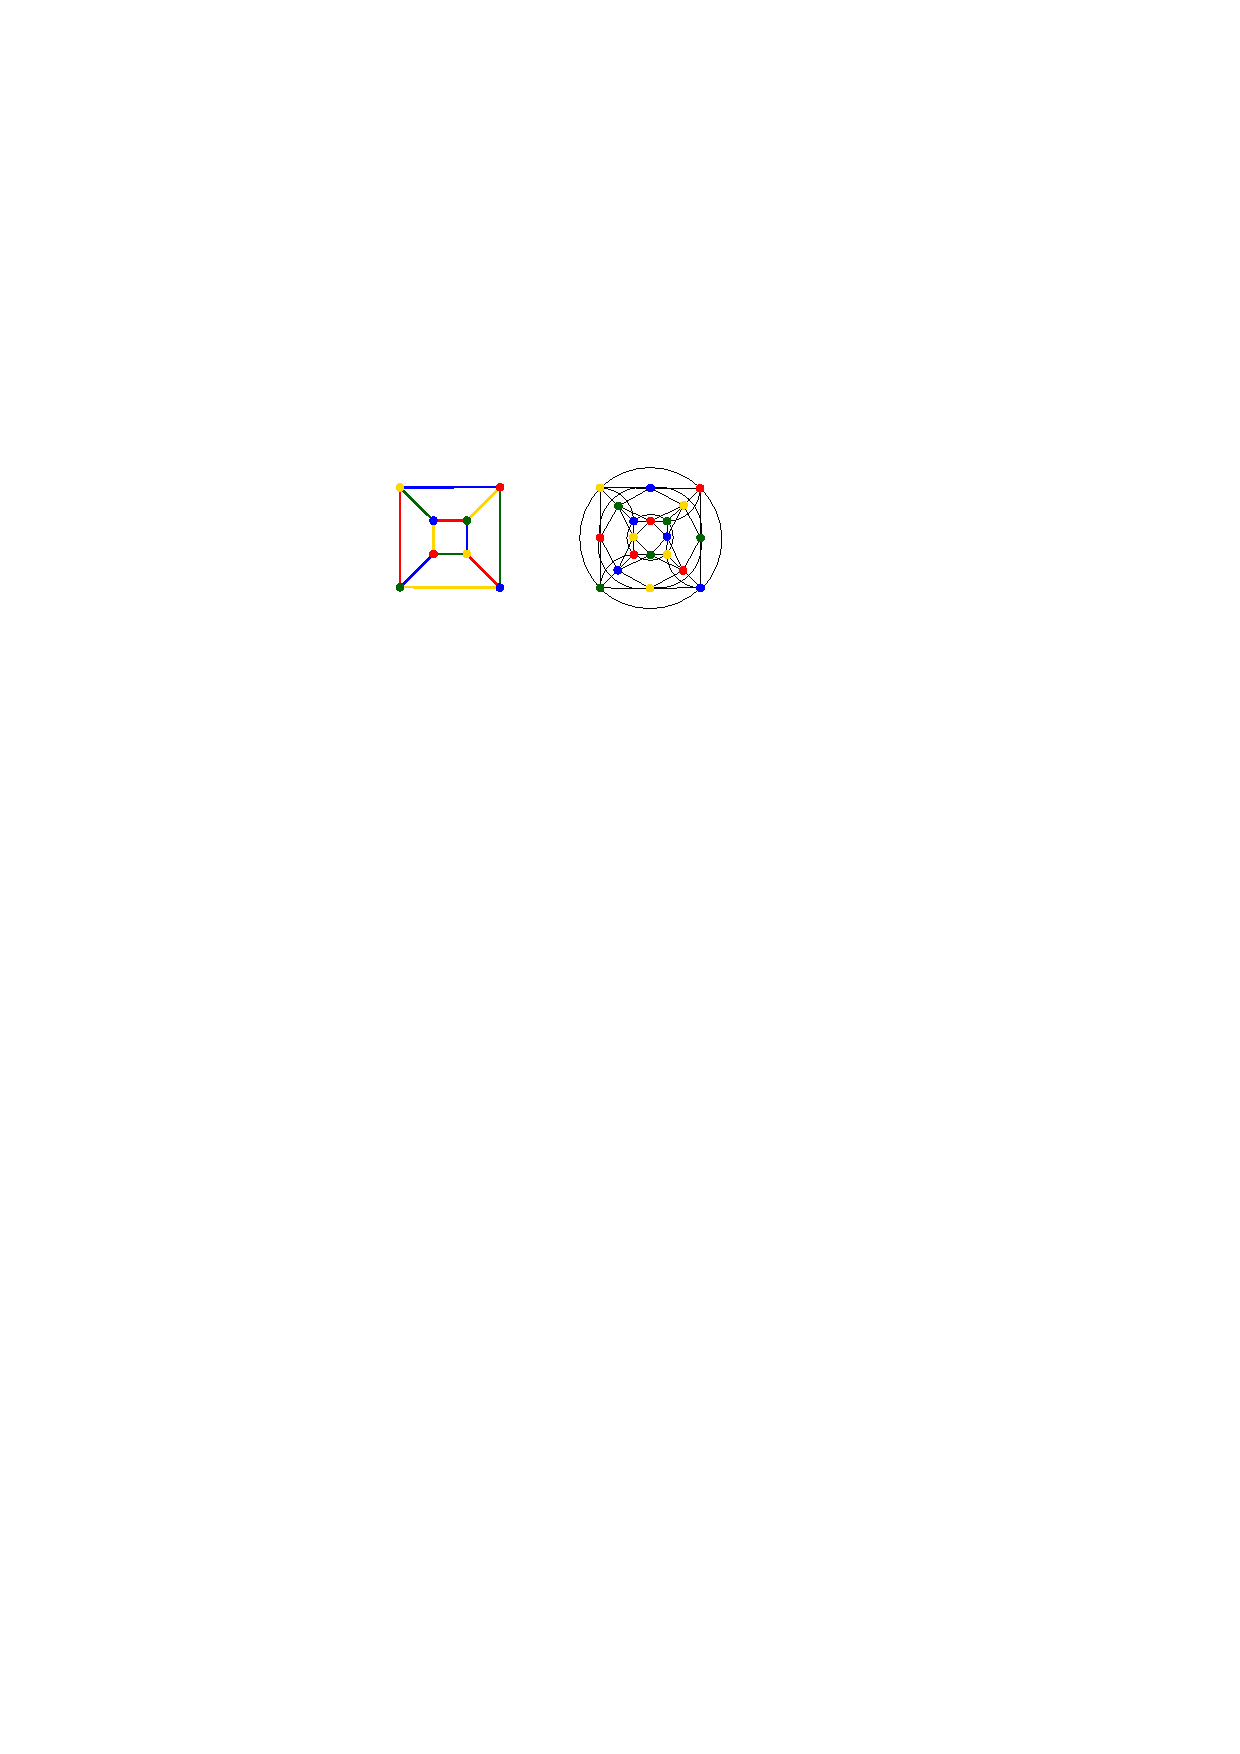
\includegraphics[width=0.6\textwidth]{../Resources/Figs/cubical_tot_g_clring_opt.pdf}
    \caption{Correspondence between the total coloring of the original graph and the vertex coloring of its total graph.}
    \label{fig:cubical_tot_g_clring}
\end{figure}

\section{Face coloring to vertex coloring}

For the conversion from face coloring to vertex coloring, we apply the same idea as when constructing line graphs. However, since the elements being colored are faces rather than edges, we need to encode adjacency of faces into the new graph by adding edges where necessary. The resulting graph is called the \textit{dual graph}.

\begin{defn}[dual graph]
    For a plane graph $G = (V, E, F)$, we define its \emph{dual graph} $G_D = (V_D, E_D)$ as follows:
    \begin{enumerate}
        \item $V_D := F$
        \item $E_D := \{ \{R_1, R_2\} \in \binom{F}{2} : \bnd(R_1) \cap \bnd(R_2) \neq \emptyset \}$
    \end{enumerate}
\end{defn}

\begin{figure}[H]
    \centering
    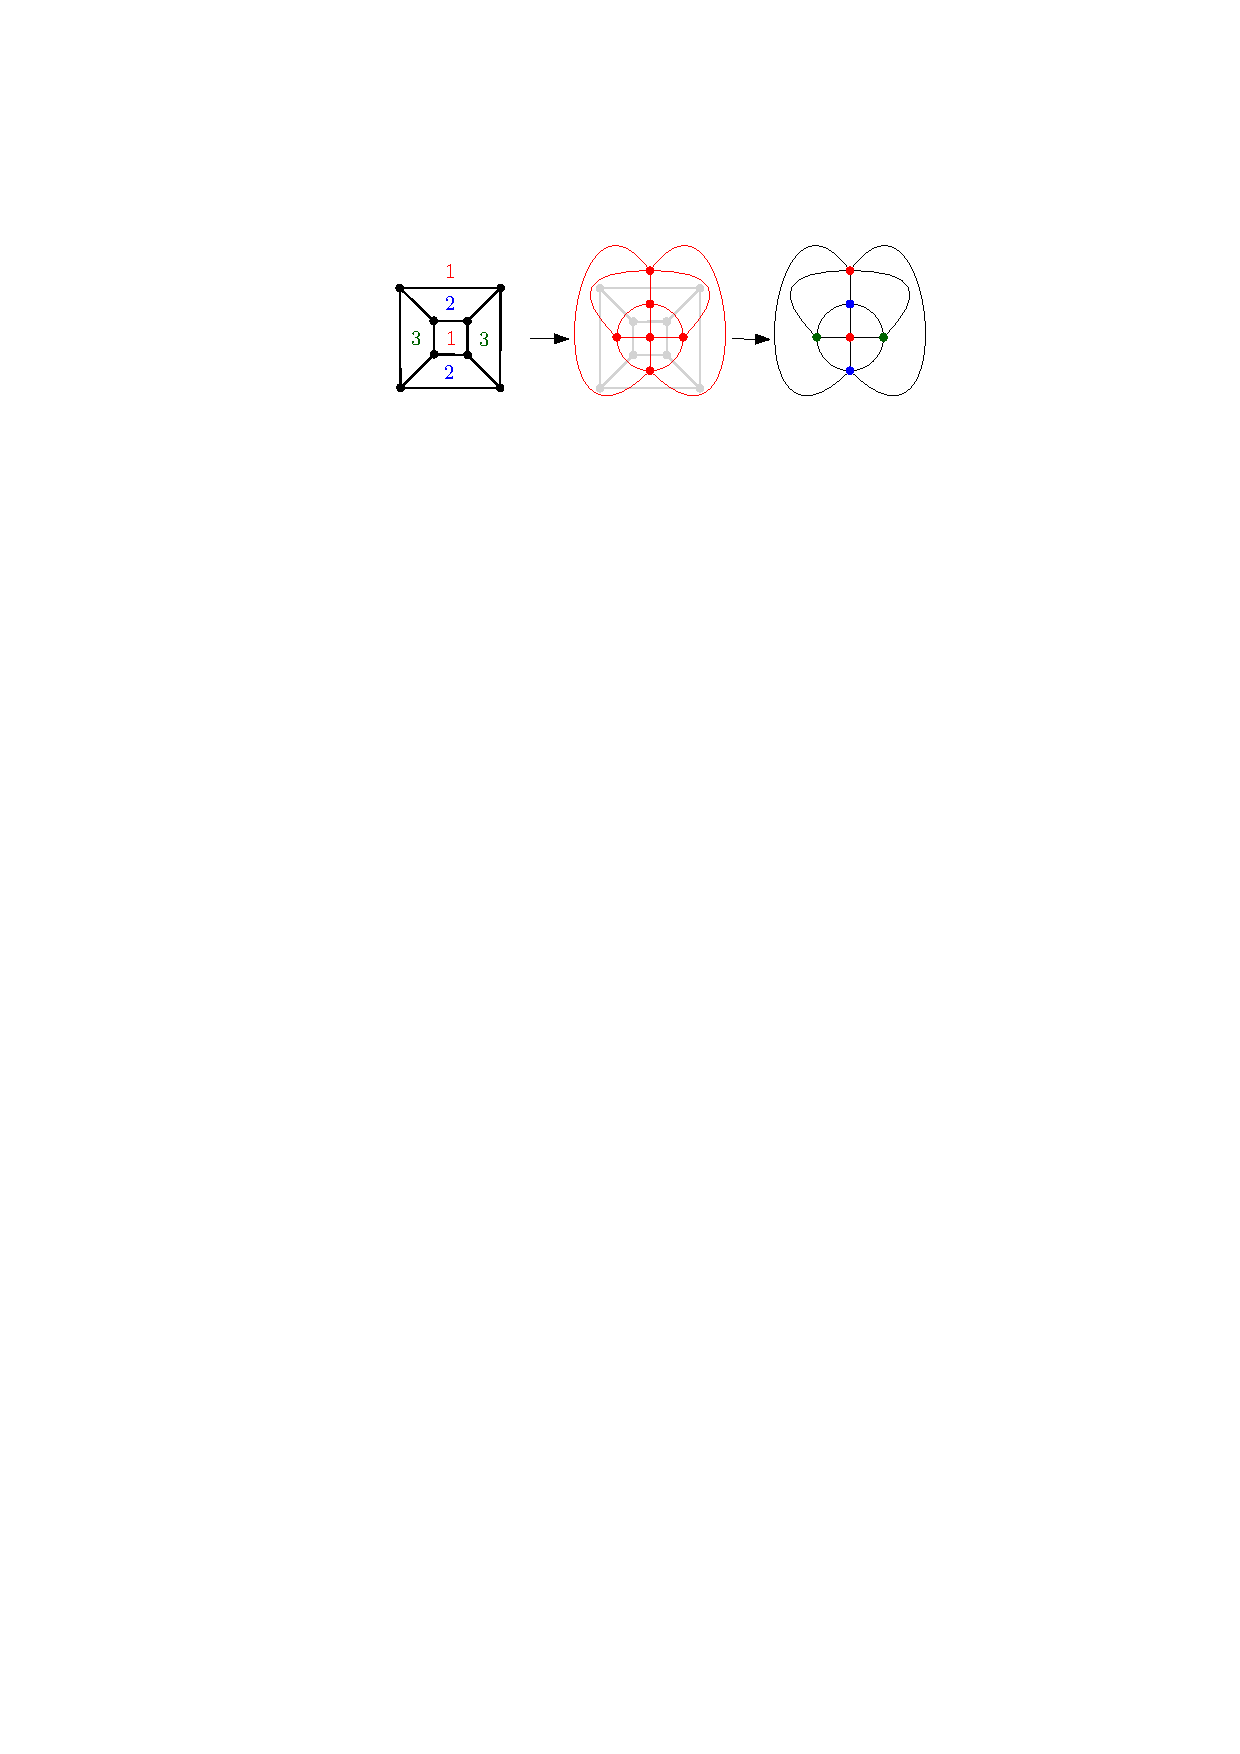
\includegraphics[width=1\textwidth]{../Resources/Figs/cubical_dual_graph.pdf}
    \caption{Visualization of conversion from face coloring to vertex coloring using a dual graph}
    \label{fig:cubical_dual_graph}
\end{figure}
\chapter{Chromatic numbers and chromatic polynomials}

\section{Computing chromatic numbers}

The vertex, edge and total chromatic numbers can be computed using the \textit{SageMath} \cite{sagemath} function called \verb|chromatic_number| and appropriate conversions from chapter \ref{chap:clring_conversions}. Computing tables \ref{tab:platonic-chrom-nums} and \ref{tab:archimedean-chrom-nums} took less than five seconds on a computer with the Apple M2 chip.

The following two tables provide overview of vertex, edge and total chromatic numbers, denoted by $\chi(G)$, $\chi'(G)$ and $\chi''(G)$ respectively, for Platonic and Archimedean solids. Note that the edge chromatic number $\chi'(G)$ is also called the \textit{chromatic index}.

\begin{table}[H]
\centering
\begin{tabular}{l@{\hspace{1.5cm}}ccc}
\toprule
\textbf{Platonic} & \textbf{$\chi(G)$} & \textbf{$\chi'(G)$} & \textbf{$\chi''(G)$} \\
\midrule
tetrahedron & 4 & 3 & 5 \\
octahedron & 3 & 4 & 5 \\
cube & 2 & 3 & 4 \\
icosahedron & 4 & 5 & 6 \\
dodecahedron & 3 & 3 & 4 \\
\bottomrule
\end{tabular}
\caption{Vertex and edge chromatic numbers of Platonic graphs}
\label{tab:platonic-chrom-nums}
\end{table}

\begin{table}[H]
\centering
\begin{tabular}{l@{\hspace{1.5cm}}ccc}
\toprule
\textbf{Archimedean} & \textbf{$\chi(G)$} & \textbf{$\chi'(G)$} & \textbf{$\chi''(G)$} \\
\midrule
truncated tetrahedron & 3 & 3 & 4 \\
cuboctahedron & 3 & 4 & 5 \\
truncated cube & 3 & 3 & 4 \\
truncated octahedron & 2 & 3 & 4 \\
rhombicuboctahedron & 3 & 4 & 5 \\
snub cube & 3 & 5 & 6 \\
icosidodecahedron & 3 & 4 & 5 \\
truncated cuboctahedron & 2 & 3 & 4 \\
truncated icosahedron & 3 & 3 & 4 \\
truncated dodecahedron & 3 & 3 & 4 \\
rhombicosidodecahedron & 3 & 4 & 5 \\
snub dodecahedron & 4 & 5 & 6 \\
truncated icosidodecahedron & 2 & 3 & 4 \\
\bottomrule
\end{tabular}
\caption{Vertex and edge chromatic numbers of Archimedean graphs}
\label{tab:archimedean-chrom-nums}
\end{table}

Note, that from the tables above, we see that indeed all the above graphs have $\chi(G)$ at most 4. This is due to the famous \textit{Four Color Theorem} \cite{appelhaken76} for planar graphs.

Note that by using the results of the \textit{Brook's theorem} \cite{brooks41}, we have that the only graph from the table above s.t. it has $\chi(G) = \Delta(G) + 1$ should be the tetrahedron. This observation is indeed true, as we can check by consulting tables \ref{tab:platonic-basic-props} and \ref{tab:archimedean-basic-props}. 

As a consequence of \textit{Vizing's theorem} \cite{misra92}, for every graph $G$ with maximum degree $\Delta(G)$, we have $\Delta(G) \leq \chi'(G) \leq \Delta(G) + 1$. This implies two classes of graphs. Class one are graphs s.t. $\chi'(G) = \Delta(G)$. Class two are then graphs s.t. $\chi'(G) = \Delta(G) + 1$. What class are graphs of Platonic and Archimedean solids?

Let us compare the degrees at each vertex of the solids as shown in tables \ref{tab:platonic-basic-props} and \ref{tab:archimedean-basic-props} with their calculated chromatic indices in the tables above. We can observe, that all the solids are of Vizing class one. Note that this is not the case for all planar graphs. In fact, there exist planar graphs with $\Delta(G)$ from 2 up to 5 such that they are class two.

Similarly, for total coloring, Vizing's conjecture \cite{vizing68} states, that for all graphs, we have $\Delta(G) + 1 \leq \chi''(G) \leq \Delta(G) + 2$. If the conjecture holds, then it again implies two classes of graphs. In the case of Platonic and Archimedean solids, it turns out, that all of them except the tetrahedron belong to class with $\chi''(G) = \Delta(G) + 1$.

\section{Formula for computing chromatic polynomials}

Chromatic polynomial of any graph $G=(V,E)$ can be calculated recursively using the following fact: When we fix two vertices $u$, $v$ s.t. $\{u,v\} \notin E$, we can split all colorings of $G$ into two disjoint groups. Let $d$ be the number of colorings of $G$ in which $u$ and $v$ are colored by different color and let $s$ be the number of colorings in which $u$ and $v$ are colored by same colors. Then the number of all colorings $P(G,x) = d + s$. Let $G+\{u,v\}$ be graph $G$ s.t. its set of edges is $E \cup \{u,v\}$. Let $G \cdot \{u,v\}$ be the graph $G + \{u,v\}$ where the edge $\{u,v\}$ is contracted into a single vertex. Then we can see that $d = P(G + \{u,v\},x)$ and $s = P(G \cdot \{u,v\},x)$. This fact yields the following formula \cite{chartrand2019}:
\begin{equation}\label{eqn:chrom_poly_nonedge}
 P(G,x) = P(G + \{u,v\},x) + P(G \cdot \{u,v\},x)
\end{equation}

The formula above serves as the recursive case of our computation i.e. when the graph has some non-edge. In the other case, the base case, the graph has no non-edges and thus it is a complete graph $K_n$ for some $n \in \mathbb{N}$. Then the chromatic polynomial is $P(K_n,x) = x \cdot (x-1) \cdot \ldots \cdot (x-n+1)$.

Consider this example: Given the graph of tetrahedron $K_4$ and $X$ the family of proper vertex colorings. The chromatic polynomial $P_{X}(K_4,x) = x \cdot (x-1) \cdot (x-2) \cdot (x-3)$. This can be seen if we label the vertices $v_1,v_2,v_3,v_4$ and imagine coloring them sequentially in the order of their labels. We have exactly $x$ colors left to use for the first vertex. With each other vertex, we have one less color available to use. 

\section{Chromatic polynomial of complete k-partite graphs with partition size 2}

In the following, let $\oplus$ denote the edge addition operation and let $\star$ denote the vertex identification operation. Let $G_{\oplus,\bar{e}}$ and $G_{\star,\bar{e}}$ describe the resulting graphs by applying the corresponding operation on some non-edge $\bar{e}$ of $G$. Let $\bar{E}$ denote the set of all non-edges of $G$.
\begin{defn}[set of non-edges]
    Let $G=(V,E)$ be a graph. We denote $\bar{E} = \bar{E}(G) = \binom{V}{2} \setminus E$ the set of non-edges of $G$.
\end{defn}

\begin{defn}[vertex identification operation]
    For a graph $G=(V,E)$ and a non-edge $\{u,v\}$ we define the resulting graph $G_{\star,\{u,v\}} = (V',E')$ as follows:
    \begin{enumerate}
        \item $V' := (V \setminus \{u,v\}) \cup \{w\}$
        \item $E' = (\binom{V'}{2} \cap E) \cup \{\{w,x\} : \{u,x\} \in E \vee \{v,x\} \in E\}$
    \end{enumerate}
    In the above, we assume that $w \notin V$.
\end{defn}

Notice, for each $\bar{e} = \{u,v\}\in \bar{E}(G)$ it holds that $|\bar{E}(G_{\star,\bar{e}})| < |\bar{E}(G)|$. This is because $\{u,v\} \notin \bar{E}(G_{\star,\bar{e}})$ and also for the new vertex $w$, we have: \[\{w,x\} \in \bar{E}(G_{\star,\bar{e}}) \implies \{u,x\} \in \bar{E}(G) \wedge \{v,x\} \in \bar{E}(G)\]
In other words, the number of non-edges after $\star$ operation always decreases.

\begin{lemma}
\label{lemma:non-edge_set_size}
    Let $G = K_{k \times (<n)}$ be a complete $k$-partite graph where each independent set has size at most $n$. Then for any non-edge $\bar{e} \in \bar{E}(G)$ and $o \in \{\oplus,\star\}$ we have that: \[|\bar{E}(G_{o,\bar{e}})| = |\bar{E}(G)| - 1\]
\end{lemma}

\begin{proof}
    Let us consider any $\bar{e} \in \bar{E}$. The operation $\oplus$ removes $\bar{e}$ from $\bar{E}$ and keeps the other non-edges intact, so the lemma holds for this case. For the case of $\star$ operation, $\bar{E}(G_{\star,\bar{e}})$ will no longer contain the non-edge $\bar{e}=\{v,u\}$. Also, since the graph is complete $k$-partite, there exists no $w \in V(G) \setminus \{v,u\}$ s.t. $\{w,v\} \in \bar{E}$ or $\{w,u\} \in \bar{E}$. This means that after the $\star$ operation, all other non-edges will stay being non-edges. Also the $\star$ operation does not create any new non-edges. This concludes the proof.
\end{proof}

\begin{lemma}
\label{lemma:indistinguishability}
    Let $G = K_{k \times (<n)}$ be a complete $k$-partite graph where each independent set has size at most $n$. Then for any two non-edges $\bar{e},\bar{f} \in \bar{E}(G)$ and $o \in \{\oplus,\star\}$ we have that: 
    \[ G_{o,\bar{e}} = G_{o,\bar{f}}\]
\end{lemma}

\begin{proof}
    Both $\bar{e}$ and $\bar{f}$ are non-edges between vertices from partitions of size $2$. Such partitions are all indistinguishable so the resulting graph is the same in both case $G_{o,\bar{e}}$ and $G_{o,\bar{f}}$.
\end{proof}

\begin{claim}
    Let $K_{k \times 2}$ be a complete $k$-partite graph where each independent set has size $2$. Then it holds that: 
    \begin{equation}\label{eqn:chromatic-pascal}
        P(K_{k \times 2},x) = \sum_{i=0}^{k} \binom{k}{i} P(K_{2k-i},x)
    \end{equation}
\end{claim}

\begin{proof}
    We base our proof on using the recursive algorithm for computing chromatic polynomials using the formula \ref{eqn:chrom_poly_nonedge} above. Let $G_{o_1,\ldots,o_n}$ be a graph resulting from applying operations $o_1$ to $o_n$ in the corresponding order. By using Lemma \ref{lemma:indistinguishability} this graph is well defined, as the resulting graph is always the same irrespective of the particular choice of non-edges we apply the operations $o_1, \ldots,o_n$ to.

    In every step of the recursion, we split the problem of calculating $P(G,x)$ to calculating the sum of $P(G_{\oplus,\bar{e}},x)$ and $P(G_{\star,\bar{e}},x)$. The recursion stops when there exists no non-edge $\bar{e} \in \bar{E}$ i.e. $G$ is a complete graph. By Lemma \ref{lemma:non-edge_set_size}, the recursion depth is equal to the number of non-edges of the original graph $K_{k\times 2}$ for every branch of the recursion. For $K_{k\times 2}$ this is equal to $k$. This means, that each branch of the recursion ends with a graph $G_{o_1,\ldots,o_k}$ where $o_i \in \{\oplus,\star\}$. For a sequence of operations $s=o_1,\ldots,o_k$ let us denote $s_{\star} = |\{ i : o_i   =\star\}|$ i.e. the number of vertex identification operations performed throughout the sequence. Then we have $G_s = K_{2k-s_{\star}}$ because every $\star$ operation removes exactly one vertex from the original graph. Let $S$ be the set of all possible sequences of $k$ operations. Then for $G=K_{k\times 2}$, we have $P(G,x)= \sum_{s\in S}P(G_s,x)$. This follows from the fact, that there is a one-to-one correspondence between branches of the recursion and sequences in $S$. We get the final formula by identifying all sequences with the same number of $\star$ operations, which yields the binomial coefficients in the final formula. 
\end{proof}


A particular example that demonstrates the claim above is the graph of octahedron $K_{2,2,2} = K_{3 \times 2}$. According to formula \ref{eqn:chromatic-pascal}, we have \[ P(K_{3 \times 2},x) = P(K_6,x)+3P(K_5,x) + 3P(K_4,x)+P(K_3,x)\] as illustrated in the figure below.

\begin{figure}[H]
    \centering
    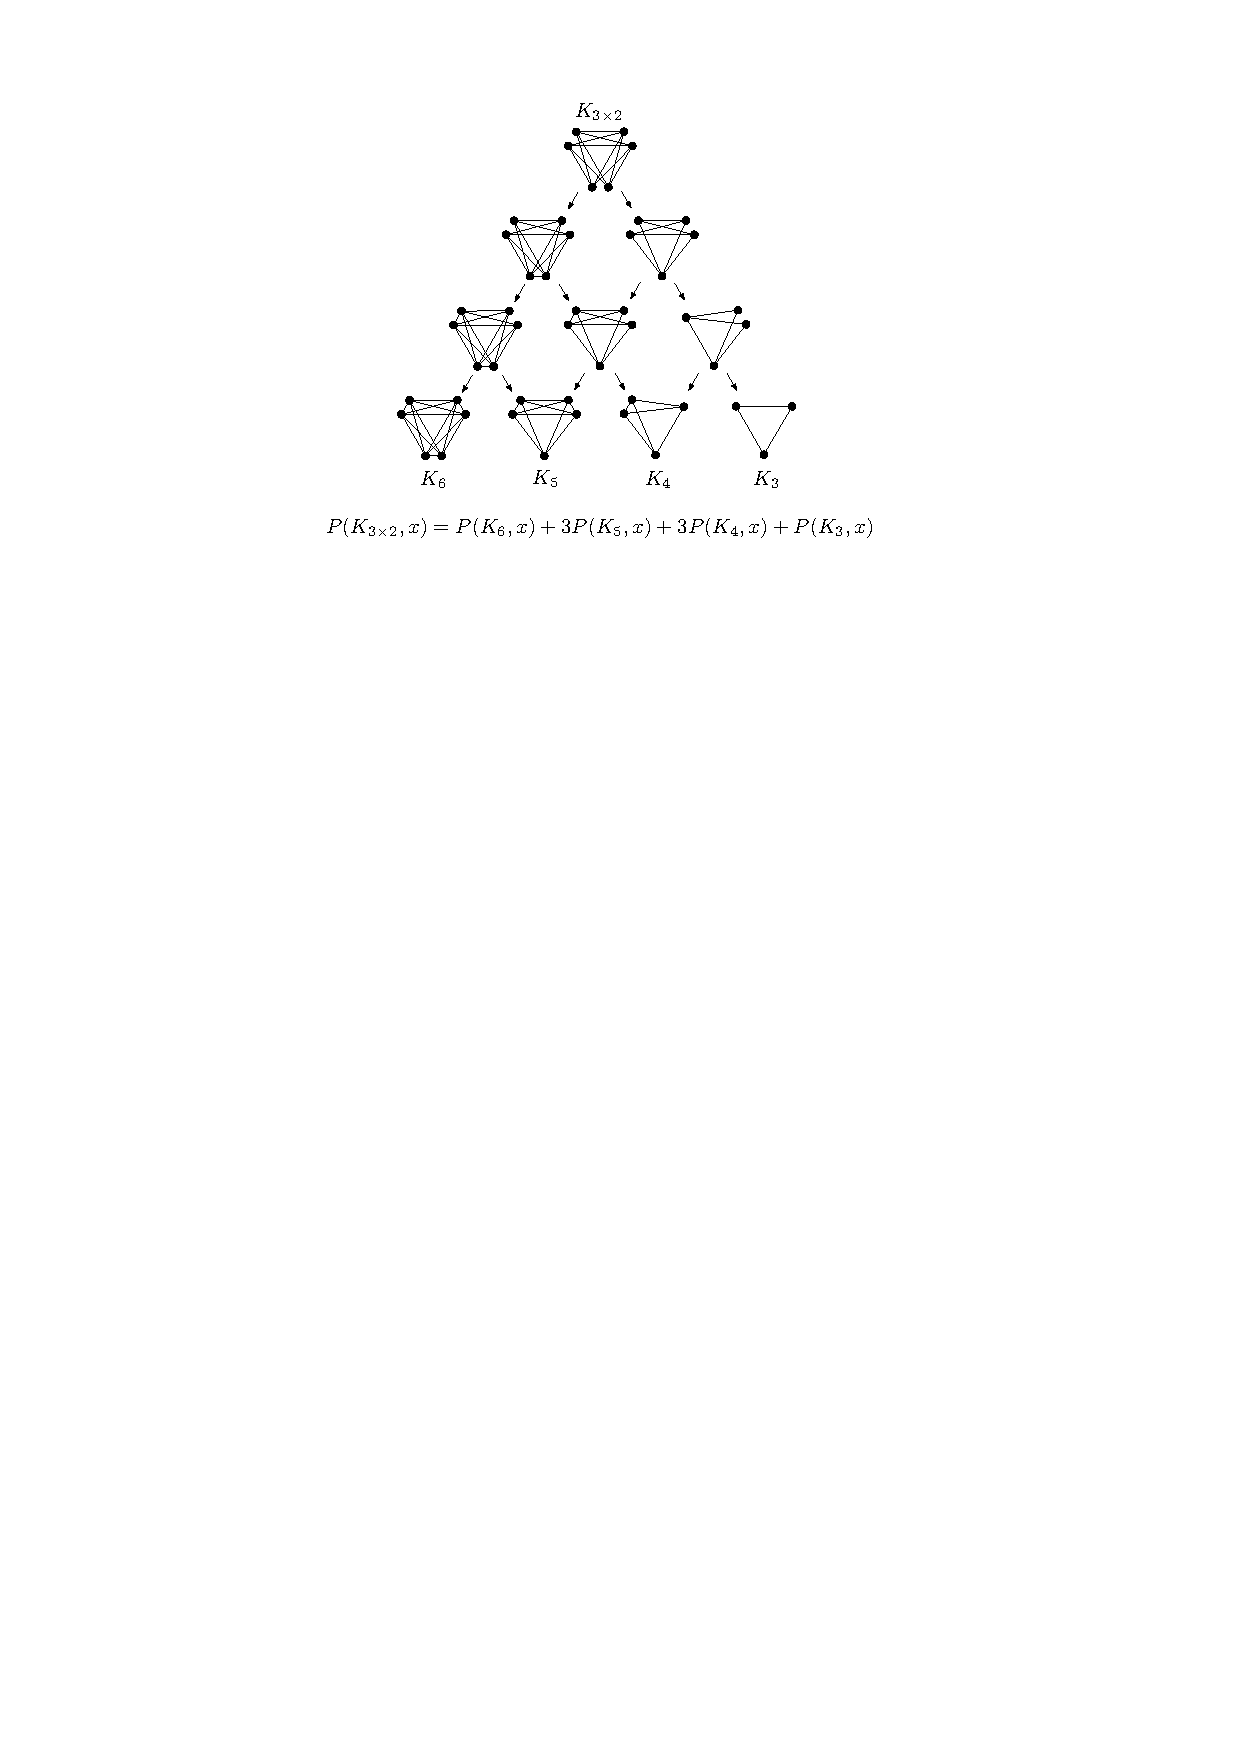
\includegraphics[width=0.8\textwidth]{Resources/Figs/octahedral_pascal_demo.pdf}
    \caption{Demonstration of formula \ref{eqn:chromatic-pascal} on a graph of the octahedron. Arrows pointing left correspond to edge additions. Arrows pointing right correspond to non-neighbor vertex identifications. Note that for some arrows, the reader must also imagine the graph being rotated after applying the corresponding operation.}
\end{figure}

\section{Computing chromatic polynomials of Platonic and Archimedean solids}

Because the graphs of Platonic and Archimedean solids are all planar, it follows, that they are also sparse. Thus, it is not practical to use the recursive formula \ref{eqn:chrom_poly_nonedge} which has complete graphs as a base case. We can instead simply reorganize the terms and instead use the following formula:

\begin{equation}\label{eqn:chrompoly-edge}
    P(G,x) = P(G - \{u,v\},x) - P(G \cdot \{u,v\},x)
\end{equation}

where $G - \{u,v\}$ is a graph with edge $\{u,v\}$ deleted and $G \cdot \{u,v\}$ a graph with edge $\{u,v\}$ contracted. 

Using the formula above, we can no longer use the complete graph as a base case. Instead we use the fact that for a tree on $n$ vertices $T_n$, we have $P(T_n,x) = x \cdot (x-1)^{n-1}$. This can be imagined by choosing a root vertex $r$ and directing all edges in $T_n$ towards $r$. Now we can color the vertices sequentially s.t. we start with $r$ and then we color direct children of $r$ and so on. To color $r$, we can use all $x$ colors. For any other vertex $v \neq r$, only the \textit{unique} parent $p$ of $v$ is colored which means that there are $x-1$ free colors for $v$. 

Note that we assume that the graph $G$ that we start with is connected. This assumption comes naturally as we are dealing only with graphs of 3-dimensional solids. We also assume that in the recursive step, we always pick an edge that lies on a cycle. This way, we will never create a disconnected graph. Finding such edge is in practice done using DFS.


An algorithm, that uses formula \ref{eqn:chrompoly-edge} and the assumptions above is implemented in the \textit{SageMath} \cite{sagemath} software under the name \verb|chromatic_polynomial|. The time complexity of this algorithm is exponential in $E(G)$, the number of edges of the graph $G$ on input. By using this algorithm, it is possible to calculate chromatic polynomials of Platonic and Archimedean graphs with at most $48$ edges in the order of minutes.

A more detailed description of how the algorithm is implemented can be found in a technical report by Read \cite{read1987chromatic}.

In the table below we provide examples of chromatic polynomials we computed.

\begin{table}[H]
\centering
\begin{tabular}{lp{0.7\linewidth}}
\toprule
\textbf{Solid} & \textbf{Chromatic polynomial} \\
\midrule
tetrahedron & $x^{4} - 6x^{3} + 11x^{2} - 6x$ \\
octahedron & $x^{6} - 12x^{5} + 58x^{4} - 137x^{3} + 154x^{2} - 64x$ \\
cube & $x^{8} - 12x^{7} + 66x^{6} - 214x^{5} + 441x^{4} - 572x^{3} + 423x^{2} - 133x$ \\
\bottomrule
\end{tabular}
\caption{Chromatic polynomial of selected solids.}
\label{tab:selected-chrom-polys}
\end{table}

\begin{highlight}

We are able to calculate also other polynomials than just the ones in the table \ref{tab:selected-chrom-polys} above. Nonetheless, these polynomials have the property, that the leading exponent is equal to the number of vertices of the graph and thus the results are complicated and hard to fit in a single table. On the other hand, we can get a sense on the number of colorings of our graphs also by evaluating the polynomials at certain points. We do this in the following section.

\section{Evaluating the chromatic polynomial}

Below we provide tables with evaluations of the chromatic polynomial of all the Platonic solids and some of the Archimedean solids. The reason is mentioned in the previous section.

\begin{table}[H]
\centering
\begin{tabular}{l@{\hspace{0.5cm}}ccccccc}
\toprule
\textbf{Platonic solid} & \textbf{2} & \textbf{3} & \textbf{4} & \textbf{5} & \textbf{6} & \textbf{7} & \textbf{8} \\
\midrule
tetrahedron & $0$ & $0$ & $24$ & $120$ & $360$ & $840$ & $1680$ \\
octahedron & $0$ & $6$ & $96$ & $780$ & $4080$ & $15330$ & $45696$ \\
cube & $2$ & $114$ & $2652$ & $29660$ & $198030$ & $932862$ & $3440024$ \\
icosahedron & $0$ & $0$ & $240$ & $80400$ & $4012560$ & $\approx 10^{7}$ & $\approx 10^{8}$ \\
dodecahedron & $0$ & $7200$ & $\approx 10^{8}$ & $\approx 10^{11}$ & $\approx 10^{13}$ & $\approx 10^{14}$ & $\approx 10^{16}$ \\
\bottomrule
\end{tabular}
\caption{Evaluated chromatic polynomial of Platonic solids at points 2 to 8.}
\label{tab:platonic-chrompolys-evals}
\end{table}

\begin{table}[H]
\centering
\begin{tabular}{l@{\hspace{0.5cm}}cccccc}
\toprule
\textbf{Archimedean solid} & \textbf{2} & \textbf{3} & \textbf{4} & \textbf{5} & \textbf{6} & \textbf{7} \\
\midrule
truncated tetrahedron & $0$ & $120$ & $60000$ & $3410880$ & $\approx 10^{7}$ & $\approx 10^{8}$ \\
cuboctahedron & $0$ & $24$ & $9216$ & $772680$ & $\approx 10^{7}$ & $\approx 10^{8}$ \\
truncated cube & $0$ & $13440$ & $\approx 10^{9}$ & $\approx 10^{13}$ & $\approx 10^{15}$ & $\approx 10^{17}$ \\
truncated octahedron & $2$ & $378978$ & $\approx 10^{10}$ & $\approx 10^{13}$ & $\approx 10^{15}$ & $\approx 10^{17}$ \\
\bottomrule
\end{tabular}
\caption{Evaluated chromatic polynomial of Archimedean solids at points 2 to 7.}
\label{tab:archimedean-chrompolys-evals}
\end{table}

It is important to note, that in table \ref{tab:platonic-polys-evals} above, in column $n$, the entry does not correspond to the amount of colorings with exactly $n$ colors but with \textbf{at most} $n$ colors. This means, that colorings that used only a proper subset of the $n$ available colors are counted as well. Sometimes, we would like to avoid counting these colorings. For this reason, we show a method to arrive at the number of colorings using \textbf{exactly} n colors, in the section below.

\section{Number of colorings using exactly n colors}
\label{sec:num-clrings-exactly-n-clrs}

\begin{defn}[number of exact n-colorings]
    Let us denote $P^*(G,n)$ the amount of colorings of graph $G$ using \textbf{exactly} $n$ colors.
\end{defn}

The number $P^*(G,n)$ can be calculated using a recursive formula with a base case being $P^*(G,\chi(G))=P(G,\chi(G))$. The recursive formula is as follows:
\begin{equation}\label{eqn:exactly-n-colors}
P^*(G,n) = P(G,n) - \sum_{i=\chi(G)}^{n-1}\binom{n}{i}P^*(G,i)    
\end{equation}

\begin{proof}
    For the base case, it is trivial to show that $P^*(G,\chi(G))=P(G,\chi(G))$ since there exist no colorings that use less than $\chi(G)$ colors.
    
    For the recursive case, let $n>\chi(G)$ be the number for which we want to calculate $P^*(G,n)$. We proceed by taking the value $P(G,n)$ and noticing, that this value also calculates colorings using $n-1$, $n-2$, \ldots \ , $\chi(G)$ colors which we want to exclude. For $i \in \{\chi(G),\ldots,n-1\}$ how many colorings using $i$ colors have we calculated? A naive approach would be to simply subtract the value $P^*(G,i)$. The problem with this approach is, that when we are allowed to use $n$ colors and have to use exactly $i$ of them, we can choose the set of $i$ colors to use in $\binom{n}{i}$ ways. Note that indeed all of the $\binom{n}{i}$ colorings use at most $n$ colors and are pairwise different. Using this observation, we can see that the correct amount to subtract is $\binom{n}{i}P^*(G,i)$ for each $i$.
\end{proof}

Now, with formula \ref{eqn:exactly-n-colors} above in hand, we can use results from tables \ref{tab:platonic-chrompolys-evals} and \ref{tab:archimedean-chrompolys-evals} to compute the numbers of colorings using \textbf{exactly} n colors. See tables below:

\begin{table}[H]
\centering
\begin{tabular}{l@{\hspace{0.5cm}}ccccccc}
\toprule
\textbf{Platonic solid} & \textbf{2} & \textbf{3} & \textbf{4} & \textbf{5} & \textbf{6} & \textbf{7} & \textbf{8} \\
\midrule
tetrahedron & $0$ & $0$ & $24$ & $0$ & $0$ & $0$ & $0$ \\
octahedron & $0$ & $6$ & $72$ & $360$ & $720$ & $0$ & $0$ \\
cube & $2$ & $108$ & $2208$ & $17520$ & $57600$ & $80640$ & $40320$ \\
icosahedron & $0$ & $0$ & $240$ & $79200$ & $3533760$ & $\approx 10^{7}$ & $\approx 10^{8}$ \\
dodecahedron & $0$ & $7200$ & $\approx 10^{8}$ & $\approx 10^{11}$ & $\approx 10^{13}$ & $\approx 10^{14}$ & $\approx 10^{16}$ \\
\bottomrule
\end{tabular}
\caption{Number of colorings of Platonic solids using \textbf{exactly} n colors for n from 2 up to 8.}
\label{tab:platonic-chrompolys-exacts}
\end{table}

\begin{table}[H]
\centering
\begin{tabular}{l@{\hspace{0.5cm}}cccccc}
\toprule
\textbf{Archimedean solid} & \textbf{2} & \textbf{3} & \textbf{4} & \textbf{5} & \textbf{6} & \textbf{7} \\
\midrule
truncated tetrahedron & $0$ & $120$ & $59520$ & $3112080$ & $\approx 10^{7}$ & $\approx 10^{8}$ \\
cuboctahedron & $0$ & $24$ & $9120$ & $726840$ & $\approx 10^{7}$ & $\approx 10^{8}$ \\
truncated cube & $0$ & $13440$ & $\approx 10^{9}$ & $\approx 10^{13}$ & $\approx 10^{15}$ & $\approx 10^{17}$ \\
truncated octahedron & $2$ & $378972$ & $\approx 10^{10}$ & $\approx 10^{13}$ & $\approx 10^{15}$ & $\approx 10^{17}$ \\
\bottomrule
\end{tabular}
\caption{Number of colorings of Archimedean solids using \textbf{exactly} n colors for n from 2 up to 7.}
\label{tab:archimedean-chrompolys-exacts}
\end{table}

\section{Limitations of the chromatic polynomial}

The results we obtained above using the chromatic polynomial have two important limitations that arise because of the way, that difference of two colorings is defined.

\subsection{Counting up to symmetries}

Firstly, it may happen, that we consider two colorings as different even though they are just different rotations or reflections of each other. See example of such colorings below:

\begin{figure}[H]
    \centering
    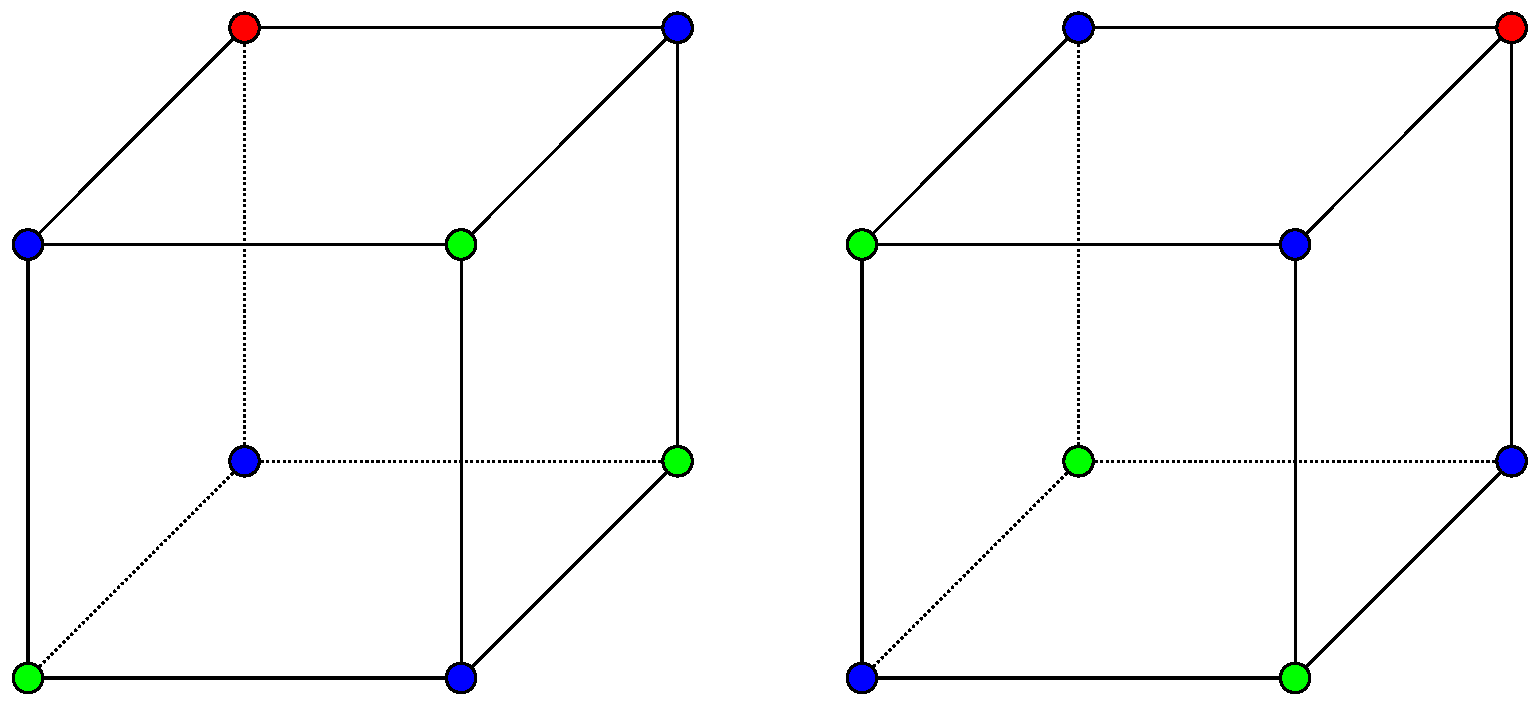
\includegraphics[width=0.75\textwidth]{Resources/Figs/cube_rotations_problem.pdf}
    \caption{Two 3-colorings of cube that are same up to symmetries}
    \label{fig:cube-clrings-same-up-to-symmetries}
\end{figure}

If we are interested only in colorings different up to symmetries, we need to use a method that is described in chapter \ref{chap:clrings-up-to-symmetries}.

\subsection{Counting up to labels of independent sets}

Second limitation arises, when we need to view the colorings as partitions into independent sets irrespective of the particular names, or values, of the colors. Then, there can be cases of partitions which we count multiple times, because there exist different non-equal ways to label the colors. In other words, an independent set that is given the color red will be considered as different from the same independent set when it is given the color blue. See illustration of this problem below:

\begin{figure}[H]
    \centering
    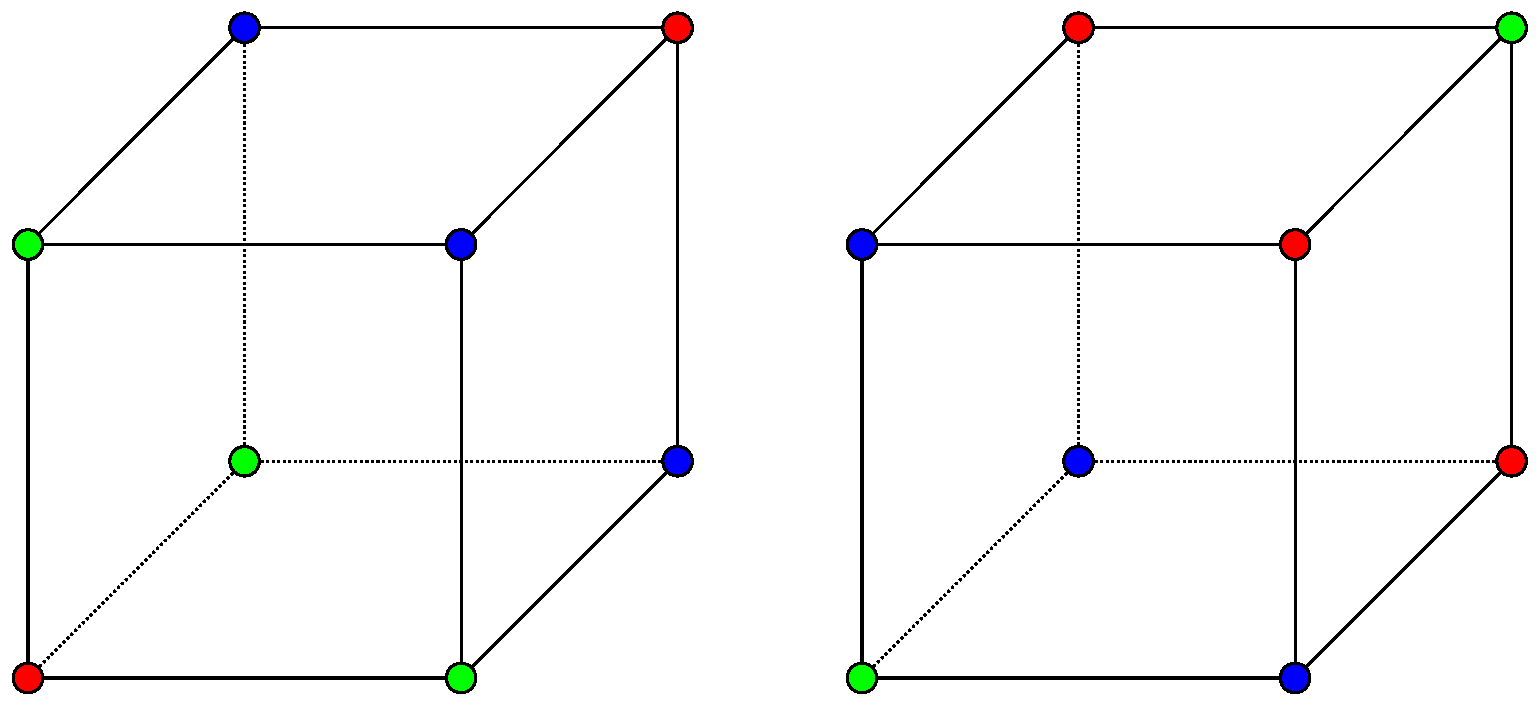
\includegraphics[width=0.75\textwidth]{Resources/Figs/cube_relabelings_problem.pdf}
    \caption{Two 3-colorings of cube that correspond to the same partition into independent sets}
    \label{fig:cube-clrings-same-partition}
\end{figure}

The problem with counting independent sets multiple times can be solved using method described in chapter \ref{chap:num-partitions-into-indep-sets}. 

Also, note that the two colorings in figure \ref{fig:cube-clrings-same-partition} above are different up to symmetries, so the problems mentioned above are indeed different and have to be handled separately.

\end{highlight}
\chapter{Number of colorings up to symmetries and the orbital chromatic polynomial}
\label{chap:clrings-up-to-symmetries}

In the previous chapters, we computed, how many proper colorings of Platonic and Archimedean solids exists using the notion of the chromatic polynomial. In that approach, we didn't take into account, that some colorings can be obtained from the other ones by simply rotating or reflecting the solid i.e. by applying some geometric transformation on it. When one coloring can be obtained from another one using some geometric transformation, then it makes good sense to regard these two colorings as identical. An analogy from chemistry is, that the properties of a molecule do not change, when we rotate it. Thus it is reasonable, to consider all its rotations as being the same molecule. 

In order to be able to say, which colorings should be considered identical, we need to define some kind of equivalence relation, that will group all the different transformations of same coloring together. In mathematics, we call this relation a \textit{transitivity relation} and its equivalence classes are typically referred to as its \textit{orbits}. The transitivity relation is defined on a set of objects, in our case the colorings, and a group that acts on these objects, the transformations.

Using the terminology above, our task boils down to counting the number of orbits of the transitivity relation, defined on colorings of our solid using the group of transformations of the solid.

To be able to use the transformations of the solids in our computations, we need a mathematical way of describing them. As we are working with graphs of the solids, we then also need to be able to describe these transformations as transformations on these graphs.


\section{Preliminaries}

It turns out, that transformations of the solid that we consider correspond exactly to automorphisms of the corresponding graph of the solid.

\begin{defn}[automorphism]
    Let $G=(V,E)$ be a graph. Then a function $f:V \rightarrow V$ is an \emph{automorphism} of $G$ if it is a bijection and for every $\{u,v\} \in E$ we have that $\{f(u),f(v)\} \in E$.
\end{defn}

For a graph $G$, we will denote the set of all automorphisms of $G$ by $\Aut(G)$.

\begin{defn}(group)
    A \emph{group} is a pair $\mathcal{G}=(G,\circ)$ where $G$ is a set, $\circ:G^2 \rightarrow G$ a binary operation s.t. the following hold:
    \begin{enumerate}
        \item $\forall x,y,z \in G : x \circ (y \circ z) = ( x \circ y ) \circ z$
        \item $\exists e \in G \ \forall x \in G :x \circ e = x = e \circ x$
        \item $ \forall x \in G \ \exists y \in G : x \circ y = e = y \circ x$
    \end{enumerate}
\end{defn}

An important observation is, that for a graph $G$, the set of all automorphisms $\Aut(G)$ together with the function composition operation forms a group. 

Before we define can define the transitivity relation, we also need to properly define the set of elements on which this relation will be defined:

\begin{defn}[colorings with up to n colors]
    For a graph $G$, positive integer $n$ and a family of colorings $C$, we define the set $C_n \subseteq C$ the set of all proper colorings of $G$ by at most $n$ colors.
\end{defn}

The definition above restricts the colorings we will be working with to finite sets only. With the notion of automorphism and colorings in hand, we can define the transitivity relation for the colorings.

\begin{defn}(transitivity relation)
        Let $G=(V,E)$ be a graph and $n\in \mathbb{N}$. Let $c_1,c_2 \in C_n$. We define $c_1 \sim c_2$ whenever exists an automorphism $\alpha \in \Aut(G) : \forall v \in V : c_1(v)=c_2(\alpha(v))$.
\end{defn}

Less formally, two colorings are related, when we can find an automorphism that maps vertices of any color in the first coloring, to vertices of the same color in the second coloring. 

We can observe, that for any coloring $c$ of $G$, we have $c \sim c$ by simply taking the identity automorphism $id \in \Aut(G)$. So the transitivity relation is \textit{reflexive}. It is also \textit{symmetric} by using the fact, that if $c_1 \sim c_2$ by existence of automorphism $\alpha$, then we can use $\alpha^{-1}$ to show that $c_2 \sim c_1$ as well. Lastly, we can also show that the relation $\sim$ is \textit{transitive}. This comes from the fact, that composing two automorphisms $\alpha$ and $\psi$ yields an automorphism. So in fact, the transitivity relation defined above is an eqivalence relation.

\begin{defn}(orbit)
    For $n \in \mathbb{N}$ and a coloring $c \in C_n$ of some graph $G$ we will call the eqivalence class $[c]_{\sim}$ an \emph{orbit} of $c$ and denote it by $\Orb(c)$.
\end{defn}

\begin{defn}(set of all orbits)
    For $n \in \mathbb{N}$ and a set $C_n$ of proper colorings of graph $G$, we denote $C_n/_\sim$ the set of all eqivalence classes of the transitivity relation $\sim$ on $C_n$.
\end{defn}

Here is a good place to point out, that it is exactly our objective, to calculate the size of this set, $\abs{C_n/_\sim}$.

\begin{defn}(stabilizer)
    For $n \in \mathbb{N}$ and a coloring $c \in C_n$ of $G=(V,E)$, we will call the set $\Stab(c) = \{ \alpha \in \Aut(G) \ | \ \forall v \in V : c(\alpha(v)) = c(v) \}$ a \emph{stabilizer} of $c$. 
\end{defn}

Again, to say more coloquially, the stabilizer is the set of all automorphisms that when applied to a coloring will result in exactly the same coloring. What we mean by same colorings is, that all the vertices get the same color under both colorings.

\section{Calculating the number of orbits}

Now, it can be shown using the Lagrange's theorem that $\abs{\Stab(c)} \cdot \abs{\Orb(c)} = \abs{\Aut(G)}$ which is the key fact that allows us to be able to compute the number of equivalence classes of the transitivity relation. Mathematically formulated, it allows us to derive the following equation:

\begin{equation}\label{eqn:orbits-by-stab}
    \sum_{c\in C_n}\abs{\Stab(c)} = \abs{\Aut(G)} \cdot \abs{C_n/_\sim} 
\end{equation}


Usually, this formula is not suitable for practical calculations because the size of set $C_n$ can be quite large. In most cases, the set $\Aut(G)$ is much smaller and thus it is more reasonable, to sum over its elements instead. 

For example, consider the graph of cube $G_{cube}$. Taking for $C_4$ the set of all proper colorings of $G_{cube}$ by at most $4$ colors, we get $\abs{C_4} = 2652$. This value can be obtained by plugging number $4$ to the chromatic polynomial of $G_{cube}$. On the other hand, by consulting table \ref{tab:plat-automorphisms} below, we have $\abs{\Aut(G_{cube})} = 48$ which is more than hundred times smaller number.

Before stating another important observation, we will need a following definition:

\begin{defn}[fixpoint]
    For a graph $G = (V,E)$, natural number $n$, a set of its proper colorings $C_n$ and automorphism $\alpha \in \Aut(G)$, we denote $\Fix(\alpha)= \{ c \in C \ | \ \forall v \in V : c(\alpha(v)) = c(v) \}$
\end{defn}

To get a formula which computes the same number but using a sum over the set $\Aut(G)$ instead, we use the following observation: The sum $\sum_{c \in C_n} \abs{\Stab(c)}$ computes the number of ordered pairs $(c,\alpha)$ s.t. $\forall v \in V : c(\alpha(v)) = c(v)$. Using the definition of fixpoint, we can calculate this number also using the sum $\sum_{\alpha \in \Aut(G)} \abs{\Fix(\alpha)}$, which yields the following important identity:
\begin{equation}\label{eqn:two-way-counting}
    \sum_{\alpha \in \Aut(G)} \abs{\Fix(\alpha)} = \sum_{c \in C_n}\abs{\Stab(c)}    
\end{equation}

By combining equations \ref{eqn:orbits-by-stab} and \ref{eqn:two-way-counting}, we get the following result, which is a direct application of the famous \textit{Burnside's lemma} on our particular setting:

\begin{thm}[application of Burnside's lemma] \label{thm:burnside}
    For a graph $G$, $n \in \mathbb{N}$ and a set of its proper colorings $C_n$, we have:
    $$\abs{C_n/_\sim} = \frac{1}{\abs{\Aut(G)}}\cdot \sum_{\alpha \in \Aut(G)}\abs{\Fix(\alpha)}$$
\end{thm}

\section{Orbital chromatic polynomial}

We introduce a notion very similar to the one of the chromatic polynomial of a graph. Additionally, we take into account symmetries.

\begin{highlight}

\begin{defn}[orbital chromatic polynomial]
    For a graph $G$ and a family of its proper colorings $C$ we define the function $OP(G,x)$ s.t. $\forall k \in \mathbb{N} : OP(G,k)$ is equal to $\abs{C_k/_\sim}$. We call this function \emph{orbital chromatic polynomial}. Indeed in Theorem \ref{thm:count-orb-chrompoly}, we show that values at every natural number correspond to the right hand side of formula \ref{eqn:oribtal-chrompoly} which is a polynomial.
\end{defn}

\end{highlight}

The notion of orbital chromatic polynomial was first introduced by Cameron and Kayibi \cite{caka2007} in 2007 and was defined in more general terms for any subgroup of automorphisms $A \leqslant  \Aut(G)$. In the following section, some of the definitions are adaptations of similar definitions also from \cite{caka2007}. The Theorem \ref{thm:count-orb-chrompoly} is equivalent to how the orbital chromatic polynomial was defined in \cite{caka2007}. In this thesis, we provide a more detailed proof of the method outlined in \cite{caka2007}. 

For a graph $G$ the orbital chromatic polynomial $OP(G,x)$ can be expressed in terms of the usual chromatic polynomial. But in order to do so, it is helpful to define a special kind of graph. We define it in terms of a given automorphism $a$ and call it the \textit{fixation graph}. Any coloring $c' \in C'_n$ of the fixation graph corresponds exactly to one coloring $c \in C_n$ of the original graph $G$ that is fixed by the automorphism $a$.

\begin{defn}[cycles of permutation]
    Given a graph $G=(V,E)$ and an automorphism $\alpha \in \Aut(G)$ we denote the set of cycles of $\alpha$ by $\Cycles(\alpha)$. By a cycle $O \in \Cycles(\alpha)$, we mean the set of vertices of $G$ on the cycle $O$.
\end{defn}

\begin{defn}[vertex set identification]
    For a graph $G=(V,E)$ a subset of vertices $S \subseteq V$ we define the \emph{identification of vertex set $S$} into a new vertex $w \notin V$ as the operation that results in a graph $G_{\star,S}=(V',E')$ defined as follows:
    \begin{enumerate}
        \item $V' := (V \setminus S) \cup \{w\}$
        \item $E' := \left( \binom{V'}{2} \cap E\right) \cup \{ \{w,x\} \ | \ (\exists x \in V \setminus S)(\exists s \in S): \{x,s\} \in E\}$
    \end{enumerate}
\end{defn}

Given a graph $G=(V,E)$ and a sequence of disjoints subsets $S_1, \ldots , S_n \subseteq V$, we denote $G_{\star,S_1,\ldots,S_n}$ the graph resulting from successive application of vertex set identification operation on the sets $S_1$ up to $S_n$ and graph $G$.

\begin{defn}[independent set]
    For a graph $G=(V,E)$ and a subset of vertices $S \subseteq V$, we say that $S$ is \emph{independent} if $\forall x,y \in S : \{x,y\} \notin E$.
\end{defn}

In the following definition, we extend the definition of an undirected graph to allow also \textit{loops}. By a loop $l \in \binom{E}{1}$, we mean an edge with both endpoints being an identical vertex. For any graph $G$ containing a loop $l$, we set the chromatic polynomial $P(G,x) = 0$.

\begin{defn}[fixation graph]
    Given a graph $G$ and automorphism $\alpha \in \Aut(G)$. For $n = \abs{\Cycles(\alpha)}$ let $O_1, \ldots ,O_n \subseteq \Cycles(\alpha)$ be the sequence of cycles of $\alpha$ in an arbitrary order. We define the \emph{fixation graph} $G /_{\alpha}$ as $G_{\star,O_1, \ldots , O_n}$ s.t. additionally, we add a loop at every new vertex $w_i$ if $O_i$ was not an independent set.
\end{defn}

Now we are ready to state the following theorem:

\begin{highlight}

\begin{thm}[computation of orbital chromatic polynomial] \label{thm:count-orb-chrompoly}
    Let $G$ be a graph, then for any natural number $n$, the following formula holds:
    \begin{equation} \label{eqn:oribtal-chrompoly}
        OP(G,n) = \frac{1}{\abs{\Aut(G)}} \cdot \sum_{\alpha \in \Aut(G)}P(G/_\alpha,n)
    \end{equation}
\end{thm}

\end{highlight}

\begin{proof}

    Let $G=(V,E)$ be a graph and $n \in \mathbb{N}$. By definition of orbital chromatic polynomial we have $OP(G,n) = \abs{C_n /_{\sim}}$. So by the Burnside's orbit counting lemma \ref{thm:burnside} we have:
    $$OP(G,n) = \frac{1}{\abs{\Aut(G)}} \cdot \sum_{\alpha \in \Aut(G)} \abs{\Fix(\alpha)}$$

    In order to prove the equation above, it is enough to show that $\forall \alpha \in \Aut(G) : P(G/_{\alpha},n) = \abs{\Fix(\alpha)}$. Formally, we need to find a one-to-one correspondence between any coloring $c \in \Fix(\alpha)$ and a coloring $c' \in C'_n$ where $C'_n$ is the set of all colorings of $G /_\alpha = (V',E')$ using at most $n$ colors. It will be helpful, for $k = \abs{\Cycles(\alpha)}$, to denote $w_1, \ldots , w_k$ the new vertices corresponding to the cycles $O_1, \ldots ,O_k \in \Cycles(\alpha)$ that were identified in $G$ to get the resulting graph $G/_\alpha$.
    
    Let $c \in \Fix(\alpha)$ be a coloring of $G$ that is fixed by $\alpha$. Because $c$ is fixed by $\alpha$, then by definition, it must hold that $\forall v \in V : c(\alpha(v)) = c(v)$. By this condition, for a given cycle $O_i \in \Cycles(\alpha)$, we have that $\forall u,v \in O_i : c(u) = c(v) = b_i$ for some color $b_i$ i.e. all vertices on a cycle must have the same color $b_i$. Note that we allow for $i \neq j$ to have $b_i = b_j$. Now we map the proper coloring $c \in C_n$ to a coloring $c' \in C'_n$ defined s.t. $\forall i \in \{1, \ldots ,k\} : c'(w_i) = b_i$. This results in a proper coloring since if for any $i \neq j$ we have $\{w_i,w_j\} \in E'$ then there must exist vertices $u \in O_i$ and $v \in O_j$ s.t. $\{u,v\} \in E$ by the definition of vertex set identification operation. Thus we have $b_i \neq b_j$. So we have $c' \in C'_n$. 
    
    Now suppose that we have $c_1,c_2 \in C_n$ s.t. $c_1 \neq c_2$ then the images under this mapping $c'_1,c'_2 \in C'_n$ are different so the mapping is injective.

    For surjectivity, suppose we have a proper coloring $c' \in C'_n$ of graph $G/_\alpha$. Then the preimage of $c'$ is the following coloring which we denote by $c \in C_n$: $(\forall O_i \in \Cycles(\alpha))( \forall v \in O_i) : c(v) = c'(w_i)$. It is not hard to see, by the definition of the vertex set identification operation, that the coloring $c$ is a proper coloring of $G$. Note that we also have that $c \in \Fix(\alpha)$ because we assigned all vertices on each cycle the same color.

    So we have that $\forall \alpha \in \Aut(G) : P(G/_{\alpha},n) = \abs{\Fix(\alpha)}$ which we needed to show. 
     
\end{proof}

\section{Calculating orbital chromatic polynomials}

Theorem \ref{thm:count-orb-chrompoly} can be used to derive a following algorithm:

\begin{algorithm}[H]
    \caption{Algorithm based on Theorem \ref{thm:count-orb-chrompoly} for computing the orbital chromatic polynomial $OP(G,x)$ of a given graph $G$} 
    \begin{algorithmic}[1]
        \Function{OrbitalChromaticPoly}{$x$}
            \State $p \gets 0$      
            \For{$\alpha \in \Aut(G)$}
                \State $H \gets G$
                \For{$O \in \Cycles(\alpha)$}
                    \If{$O$ not independent set}
                        \State Continue with next permutation at step $3$
                    \EndIf
                    \State $H \gets H_{\star,O}$
                \EndFor
                \State $p \gets p + P(H,x)$
            \EndFor   
            \State \Return $p$
        \EndFunction
    \end{algorithmic}
    \label{alg:orb-chrompoly}
\end{algorithm}

An implementation of the algorithm \ref{alg:orb-chrompoly} above is provided in the appendix. This implementation was used to calculate the polynomials that can be seen in table \ref{tab:selected-orbital-chrom-polys} below.

\renewcommand{\arraystretch}{2.0}
\begin{table}[H]
\centering
\begin{tabular}{l@{\hspace{1.5cm}}p{0.7\linewidth}}
\toprule
\textbf{Solid} & \textbf{Orbital chromatic polynomial} \\
\midrule
tetrahedron & $\frac{1}{24}x^{4} - \frac{1}{4}x^{3} + \frac{11}{24}x^{2} - \frac{1}{4}x$ \\
octahedron & $\frac{1}{48}x^{6} - \frac{3}{16}x^{5} + \frac{37}{48}x^{4} - \frac{79}{48}x^{3} + \frac{41}{24}x^{2} - \frac{2}{3}x$ \\
cube & $\frac{1}{48}x^{8} - \frac{1}{4}x^{7} + \frac{3}{2}x^{6} - \frac{16}{3}x^{5} + \frac{193}{16}x^{4} - \frac{203}{12}x^{3} + \frac{161}{12}x^{2} - \frac{9}{2}x$ \\
\bottomrule
\end{tabular}
\caption{Orbital chromatic polynomial of selected solids.}
\label{tab:selected-orbital-chrom-polys}
\end{table}
\renewcommand{\arraystretch}{1.0}

\section{Demonstrative example on a graph of the octahedron}

The difference between chromatic and orbital chromatic polynomials can be demonstrated on a graph of the octahedron $K_{3 \times 2}$. As can be seen in table \ref{tab:selected-chrom-polys} we have that: $$P(K_{3 \times 2},x) = x^{6} - 12x^{5} + 58x^{4} - 137x^{3} + 154x^{2} - 64x$$ whereas by \ref{tab:selected-orbital-chrom-polys} 
 we have: $$OP(K_{3 \times 2},x) = \frac{1}{48}x^{6} - \frac{3}{16}x^{5} + \frac{37}{48}x^{4} - \frac{79}{48}x^{3} + \frac{41}{24}x^{2} - \frac{2}{3}x$$.

Plugging in $3$ for $x$, we get the number of vertex colorings of the octahedron using at most $3$ colors. We get $P(K_{3 \times 2},3) = 6$. All these colorings can be enumerated using \textit{SageMath} \cite{sagemath} and its \verb|all_graph_colorings| function. On the figure below, we can see all of these $6$ colorings:

\begin{figure}[H]
    \centering
    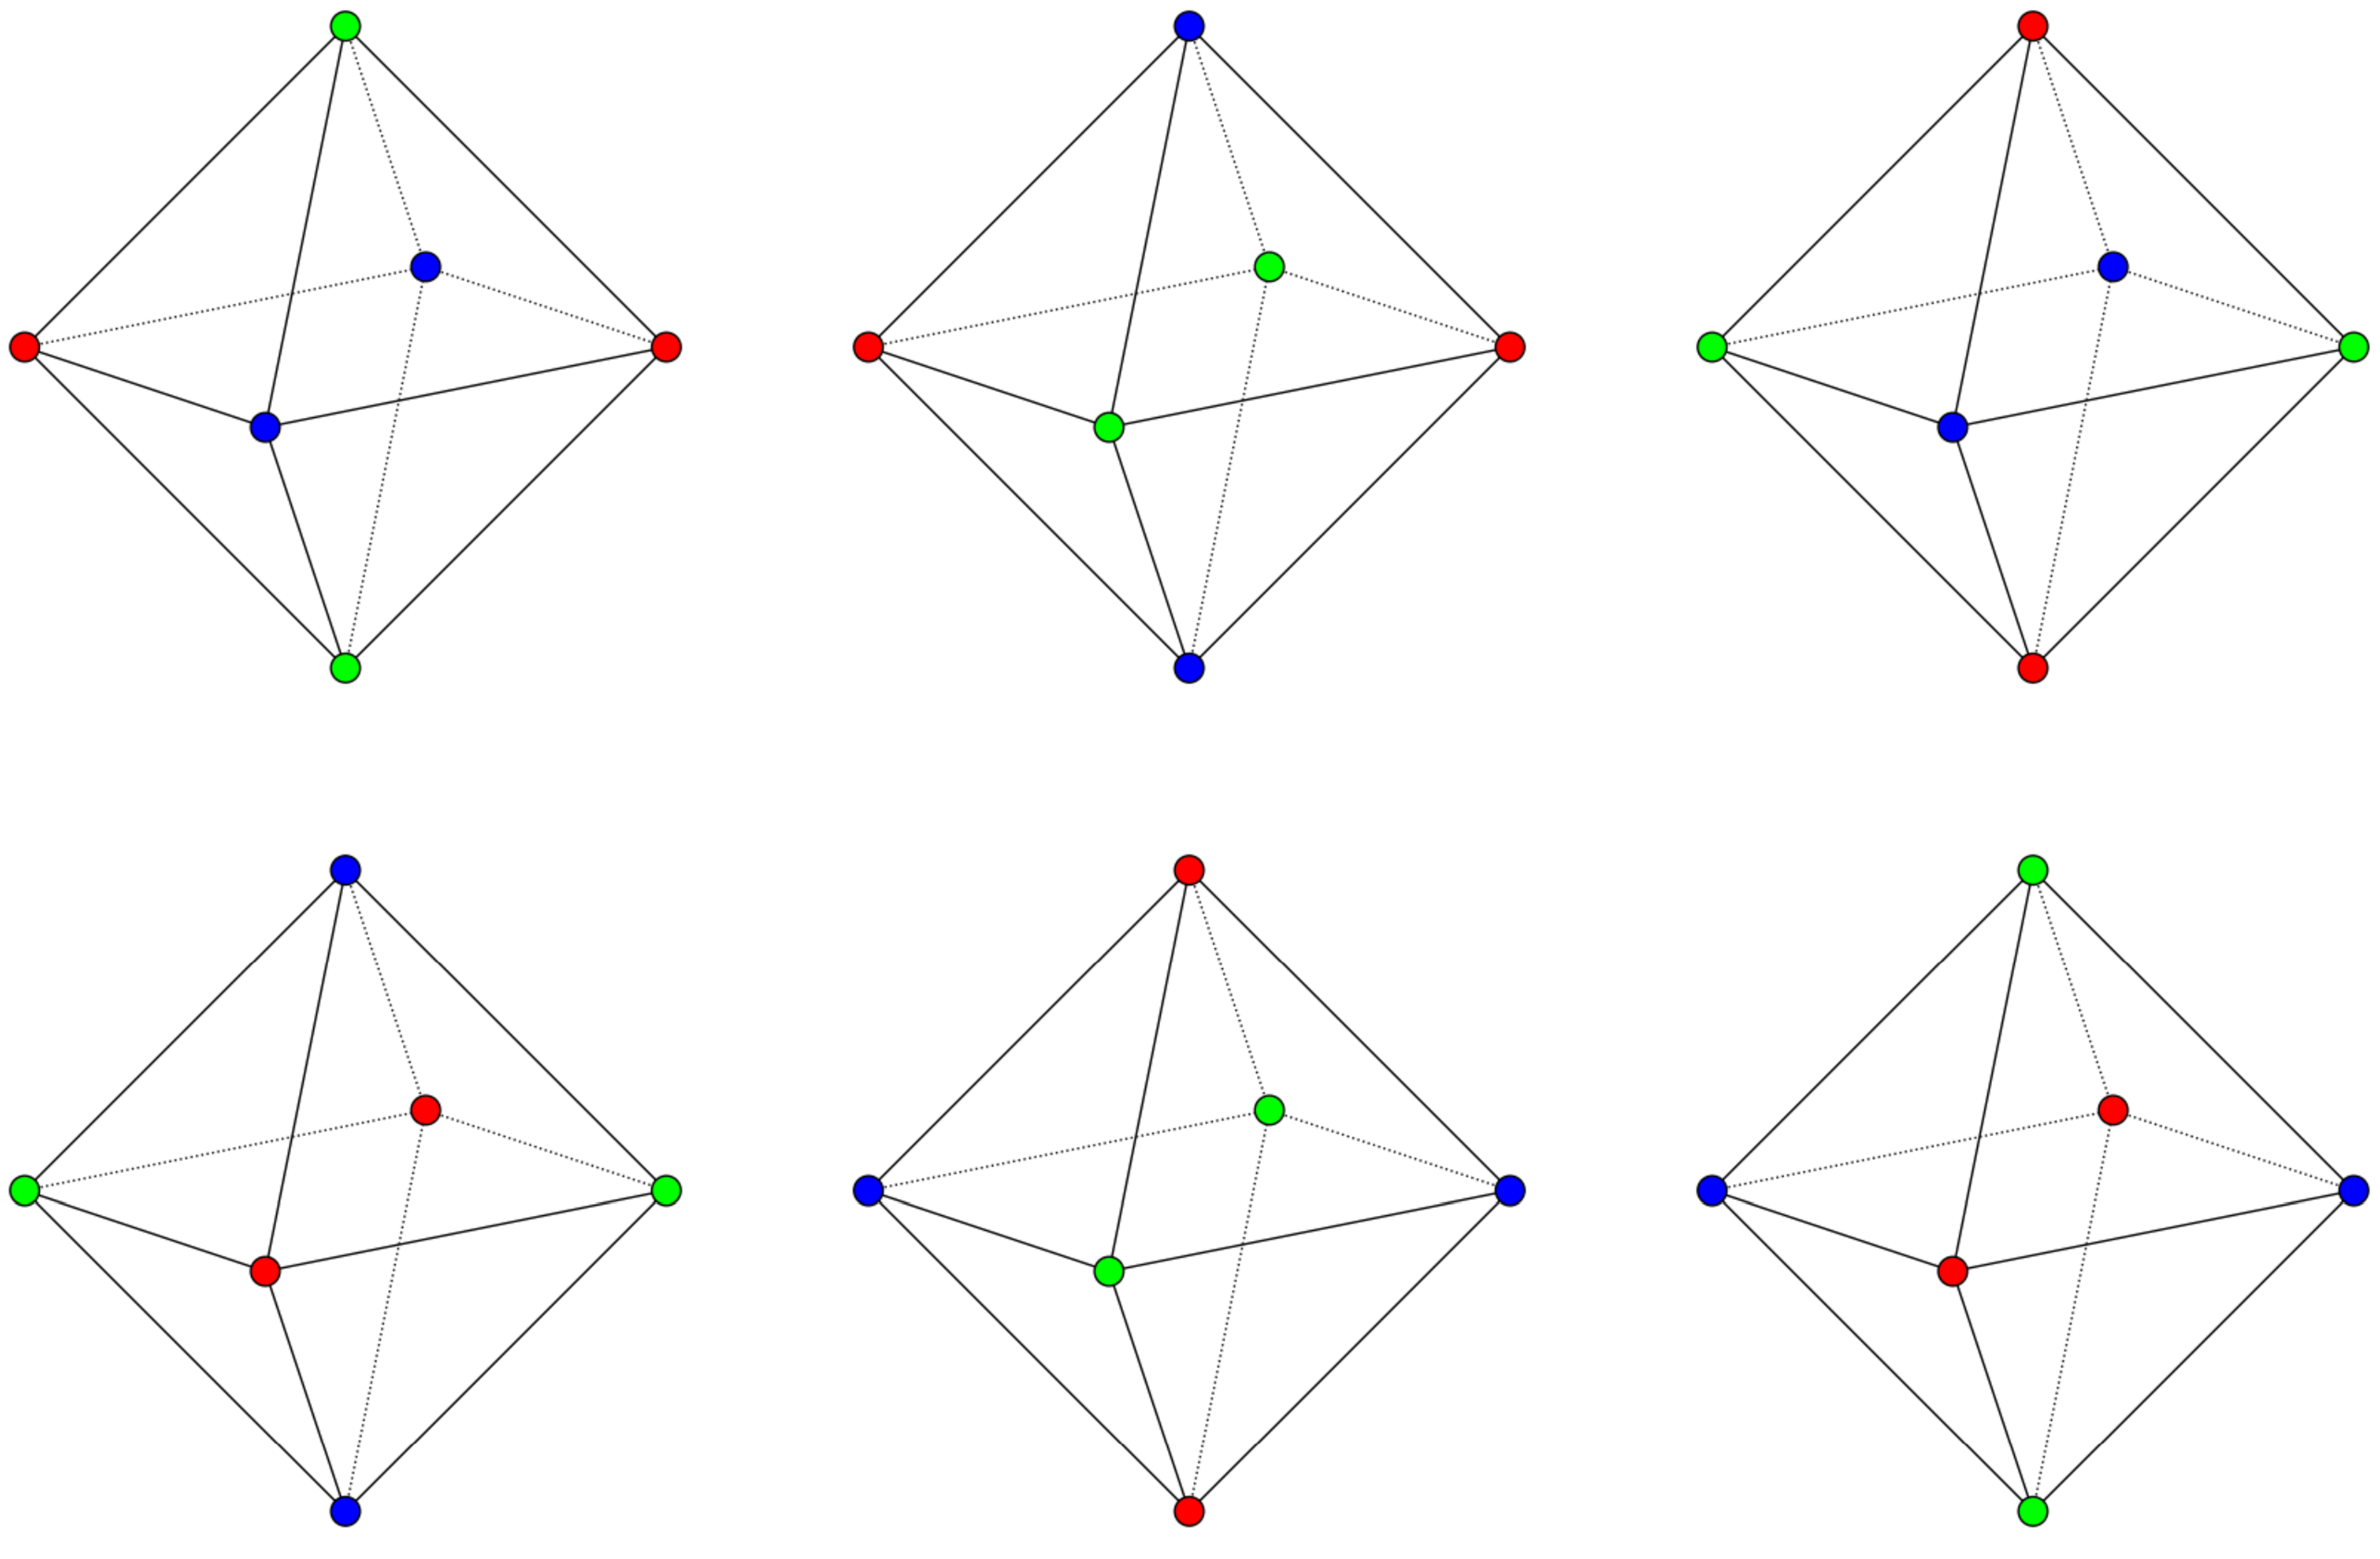
\includegraphics[width=1\textwidth]{../Resources/Figs/octahedron_3-clrings.pdf}
    \caption{All 3 colorings of octahedral graph}
    \label{fig:octahedron-3-clrings}
\end{figure}

Now, an important observation is, that all of these $6$ colorings are equivalent when considered up to automorphisms. Indeed we can compute that $OP(K_{3 \times 2},3) = 1$.

\begin{highlight}

\section{Comparison with chromatic polynomial}

It is interesting to compare the difference between chromatic polynomial and orbital chromatic polynomial for all the solids by looking at the values of the polynomials at certain points. This can be seen in table \ref{tab:platonic-polys-evals} below.

\begin{table}[H]
\centering
\begin{tabular}{l@{\hspace{0.5cm}}ccccccc}
\toprule
\textbf{Platonic solid} & \textbf{2} & \textbf{3} & \textbf{4} & \textbf{5} & \textbf{6} & \textbf{7} & \textbf{8} \\
\midrule
tetrahedron & $0$ & $0$ & $24$ & $120$ & $360$ & $840$ & $1680$ \\
 & $0$ & $0$ & $1$ & $5$ & $15$ & $35$ & $70$ \\
\specialrule{0.2pt}{0.65ex}{0.65ex}
octahedron & $0$ & $6$ & $96$ & $780$ & $4080$ & $15330$ & $45696$ \\
 & $0$ & $1$ & $10$ & $55$ & $215$ & $665$ & $1736$ \\
\specialrule{0.2pt}{0.65ex}{0.65ex}
cube & $2$ & $114$ & $2652$ & $29660$ & $198030$ & $932862$ & $3440024$ \\
 & $1$ & $15$ & $154$ & $1115$ & $5955$ & $24836$ & $85260$ \\
\specialrule{0.2pt}{0.65ex}{0.65ex}
icosahedron & $0$ & $0$ & $240$ & $80400$ & $4012560$ & $\approx 10^{7}$ & $\approx 10^{8}$ \\
 & $0$ & $0$ & $2$ & $670$ & $33444$ & $640444$ & $6878900$ \\
\specialrule{0.2pt}{0.65ex}{0.65ex}
dodecahedron & $0$ & $7200$ & $\approx 10^{8}$ & $\approx 10^{11}$ & $\approx 10^{13}$ & $\approx 10^{14}$ & $\approx 10^{16}$ \\
 & $0$ & $75$ & $1404848$ & $\approx 10^{8}$ & $\approx 10^{11}$ & $\approx 10^{12}$ & $\approx 10^{14}$ \\
\bottomrule
\end{tabular}
\caption{Evaluated chromatic polynomial and orbital chromatic polynomial for platonic solids at points 2 to 8. For each solid, the top row contains the chromatic polynomial, the bottom row contains the orbital chromatic polynoial.}
\label{tab:platonic-polys-evals}
\end{table}

Note, that we can use the same method as in section \ref{sec:num-clrings-exactly-n-clrs}, using the formula \ref{eqn:exactly-n-colors}, also for the orbital chromatic polynomial $OP(G,x)$, to arrive at corresponding values $OP^*(G,n)$. Using the formula, we can then simplify table \ref{tab:platonic-polys-evals} above to get the following table:

\begin{table}[H]
\centering
\begin{tabular}{l@{\hspace{0.5cm}}ccccccc}
\toprule
\textbf{Platonic solid} & \textbf{2} & \textbf{3} & \textbf{4} & \textbf{5} & \textbf{6} & \textbf{7} & \textbf{8} \\
\midrule
tetrahedron & $0$ & $0$ & $24$ & $0$ & $0$ & $0$ & $0$ \\
 & $0$ & $0$ & $1$ & $0$ & $0$ & $0$ & $0$ \\
\specialrule{0.2pt}{0.65ex}{0.65ex}
octahedron & $0$ & $6$ & $72$ & $360$ & $720$ & $0$ & $0$ \\
 & $0$ & $1$ & $6$ & $15$ & $15$ & $0$ & $0$ \\
\specialrule{0.2pt}{0.65ex}{0.65ex}
cube & $2$ & $108$ & $2208$ & $17520$ & $57600$ & $80640$ & $40320$ \\
 & $1$ & $12$ & $100$ & $485$ & $1290$ & $1680$ & $840$ \\
\specialrule{0.2pt}{0.65ex}{0.65ex}
icosahedron & $0$ & $0$ & $240$ & $79200$ & $3533760$ & $\approx 10^{7}$ & $\approx 10^{8}$ \\
 & $0$ & $0$ & $2$ & $660$ & $29454$ & $420336$ & $2654400$ \\
\specialrule{0.2pt}{0.65ex}{0.65ex}
dodecahedron & $0$ & $7200$ & $\approx 10^{8}$ & $\approx 10^{11}$ & $\approx 10^{13}$ & $\approx 10^{14}$ & $\approx 10^{16}$ \\
 & $0$ & $75$ & $1404548$ & $\approx 10^{8}$ & $\approx 10^{11}$ & $\approx 10^{12}$ & $\approx 10^{14}$ \\
\bottomrule
\end{tabular}
\caption{Numbers of colorings using exactly 2 to 8 colors. For each solid, the top row contains the value when counting symmetric colorings as different. The bottom row takes two colorings as different only if they cannot be identified using some automorphism.}
\label{tab:platonic-exactly-n-clrs}
\end{table}

\end{highlight}
\chapter{Orbital chromatic polynomial}

We introduce a notion very similar to the one of the chromatic polynomial of a graph. Additionally, we take into account symmetries.

\begin{highlight}

\begin{defn}[orbital chromatic polynomial]
    For a graph $G$ and a family of its proper colorings $C$ we define the function $OP(G,x)$ s.t. $\forall k \in \mathbb{N} : OP(G,k)$ is equal to $\abs{C_k/_\sim}$. We call this function \emph{orbital chromatic polynomial}. Indeed in Theorem \ref{thm:count-orb-chrompoly}, we show that values at every natural number correspond to the right hand side of formula \ref{eqn:oribtal-chrompoly} which is a polynomial.
\end{defn}

\end{highlight}

The notion of orbital chromatic polynomial was first introduced by Cameron and Kayibi \cite{caka2007} in 2007 and was defined in more general terms for any subgroup of automorphisms $A \leqslant  \Aut(G)$. In the following section, some of the definitions are adaptations of similar definitions also from \cite{caka2007}. The Theorem \ref{thm:count-orb-chrompoly} is equivalent to how the orbital chromatic polynomial was defined in \cite{caka2007}. In this thesis, we provide a more detailed proof of the method outlined in \cite{caka2007}. 

For a graph $G$ the orbital chromatic polynomial $OP(G,x)$ can be expressed in terms of the usual chromatic polynomial. But in order to do so, it is helpful to define a special kind of graph. We define it in terms of a given automorphism $a$ and call it the \textit{fixation graph}. Any coloring $c' \in C'_n$ of the fixation graph corresponds exactly to one coloring $c \in C_n$ of the original graph $G$ that is fixed by the automorphism $a$.

\begin{defn}[cycles of permutation]
    Given a graph $G=(V,E)$ and an automorphism $\alpha \in \Aut(G)$ we denote the set of cycles of $\alpha$ by $\Cycles(\alpha)$. By a cycle $O \in \Cycles(\alpha)$, we mean the set of vertices of $G$ on the cycle $O$.
\end{defn}

\begin{defn}[vertex set identification]
    For a graph $G=(V,E)$ a subset of vertices $S \subseteq V$ we define the \emph{identification of vertex set $S$} into a new vertex $w \notin V$ as the operation that results in a graph $G_{\star,S}=(V',E')$ defined as follows:
    \begin{enumerate}
        \item $V' := (V \setminus S) \cup \{w\}$
        \item $E' := \left( \binom{V'}{2} \cap E\right) \cup \{ \{w,x\} \ | \ (\exists x \in V \setminus S)(\exists s \in S): \{x,s\} \in E\}$
    \end{enumerate}
\end{defn}

Given a graph $G=(V,E)$ and a sequence of disjoints subsets $S_1, \ldots , S_n \subseteq V$, we denote $G_{\star,S_1,\ldots,S_n}$ the graph resulting from successive application of vertex set identification operation on the sets $S_1$ up to $S_n$ and graph $G$.

\begin{defn}[independent set]
    For a graph $G=(V,E)$ and a subset of vertices $S \subseteq V$, we say that $S$ is \emph{independent} if $\forall x,y \in S : \{x,y\} \notin E$.
\end{defn}

In the following definition, we extend the definition of an undirected graph to allow also \textit{loops}. By a loop $l \in \binom{E}{1}$, we mean an edge with both endpoints being an identical vertex. For any graph $G$ containing a loop $l$, we set the chromatic polynomial $P(G,x) = 0$.

\begin{defn}[fixation graph]
    Given a graph $G$ and automorphism $\alpha \in \Aut(G)$. For $n = \abs{\Cycles(\alpha)}$ let $O_1, \ldots ,O_n \subseteq \Cycles(\alpha)$ be the sequence of cycles of $\alpha$ in an arbitrary order. We define the \emph{fixation graph} $G /_{\alpha}$ as $G_{\star,O_1, \ldots , O_n}$ s.t. additionally, we add a loop at every new vertex $w_i$ if $O_i$ was not an independent set.
\end{defn}

Now we are ready to state the following theorem:

\begin{highlight}

\begin{thm}[computation of orbital chromatic polynomial] \label{thm:count-orb-chrompoly}
    Let $G$ be a graph, then for any natural number $n$, the following formula holds:
    \begin{equation} \label{eqn:oribtal-chrompoly}
        OP(G,n) = \frac{1}{\abs{\Aut(G)}} \cdot \sum_{\alpha \in \Aut(G)}P(G/_\alpha,n)
    \end{equation}
\end{thm}

\end{highlight}

\begin{proof}

    Let $G=(V,E)$ be a graph and $n \in \mathbb{N}$. By definition of orbital chromatic polynomial we have $OP(G,n) = \abs{C_n /_{\sim}}$. So by the Burnside's orbit counting lemma \ref{thm:burnside} we have:
    $$OP(G,n) = \frac{1}{\abs{\Aut(G)}} \cdot \sum_{\alpha \in \Aut(G)} \abs{\Fix(\alpha)}$$

    In order to prove the equation above, it is enough to show that $\forall \alpha \in \Aut(G) : P(G/_{\alpha},n) = \abs{\Fix(\alpha)}$. Formally, we need to find a one-to-one correspondence between any coloring $c \in \Fix(\alpha)$ and a coloring $c' \in C'_n$ where $C'_n$ is the set of all colorings of $G /_\alpha = (V',E')$ using at most $n$ colors. It will be helpful, for $k = \abs{\Cycles(\alpha)}$, to denote $w_1, \ldots , w_k$ the new vertices corresponding to the cycles $O_1, \ldots ,O_k \in \Cycles(\alpha)$ that were identified in $G$ to get the resulting graph $G/_\alpha$.
    
    Let $c \in \Fix(\alpha)$ be a coloring of $G$ that is fixed by $\alpha$. Because $c$ is fixed by $\alpha$, then by definition, it must hold that $\forall v \in V : c(\alpha(v)) = c(v)$. By this condition, for a given cycle $O_i \in \Cycles(\alpha)$, we have that $\forall u,v \in O_i : c(u) = c(v) = b_i$ for some color $b_i$ i.e. all vertices on a cycle must have the same color $b_i$. Note that we allow for $i \neq j$ to have $b_i = b_j$. Now we map the proper coloring $c \in C_n$ to a coloring $c' \in C'_n$ defined s.t. $\forall i \in \{1, \ldots ,k\} : c'(w_i) = b_i$. This results in a proper coloring since if for any $i \neq j$ we have $\{w_i,w_j\} \in E'$ then there must exist vertices $u \in O_i$ and $v \in O_j$ s.t. $\{u,v\} \in E$ by the definition of vertex set identification operation. Thus we have $b_i \neq b_j$. So we have $c' \in C'_n$. 
    
    Now suppose that we have $c_1,c_2 \in C_n$ s.t. $c_1 \neq c_2$ then the images under this mapping $c'_1,c'_2 \in C'_n$ are different so the mapping is injective.

    For surjectivity, suppose we have a proper coloring $c' \in C'_n$ of graph $G/_\alpha$. Then the preimage of $c'$ is the following coloring which we denote by $c \in C_n$: $(\forall O_i \in \Cycles(\alpha))( \forall v \in O_i) : c(v) = c'(w_i)$. It is not hard to see, by the definition of the vertex set identification operation, that the coloring $c$ is a proper coloring of $G$. Note that we also have that $c \in \Fix(\alpha)$ because we assigned all vertices on each cycle the same color.

    So we have that $\forall \alpha \in \Aut(G) : P(G/_{\alpha},n) = \abs{\Fix(\alpha)}$ which we needed to show. 
     
\end{proof}

\section{Calculating orbital chromatic polynomials}

Theorem \ref{thm:count-orb-chrompoly} can be used to derive a following algorithm:

\begin{algorithm}[H]
    \caption{Algorithm based on Theorem \ref{thm:count-orb-chrompoly} for computing the orbital chromatic polynomial $OP(G,x)$ of a given graph $G$} 
    \begin{algorithmic}[1]
        \Function{OrbitalChromaticPoly}{$x$}
            \State $p \gets 0$      
            \For{$\alpha \in \Aut(G)$}
                \State $H \gets G$
                \For{$O \in \Cycles(\alpha)$}
                    \If{$O$ not independent set}
                        \State Continue with next permutation at step $3$
                    \EndIf
                    \State $H \gets H_{\star,O}$
                \EndFor
                \State $p \gets p + P(H,x)$
            \EndFor   
            \State \Return $p$
        \EndFunction
    \end{algorithmic}
    \label{alg:orb-chrompoly}
\end{algorithm}

An implementation of the algorithm \ref{alg:orb-chrompoly} above is provided in the appendix. This implementation was used to calculate the polynomials that can be seen in table \ref{tab:selected-orbital-chrom-polys} below.

\renewcommand{\arraystretch}{2.0}
\begin{table}[H]
\centering
\begin{tabular}{l@{\hspace{1.5cm}}p{0.7\linewidth}}
\toprule
\textbf{Solid} & \textbf{Orbital chromatic polynomial} \\
\midrule
tetrahedron & $\frac{1}{24}x^{4} - \frac{1}{4}x^{3} + \frac{11}{24}x^{2} - \frac{1}{4}x$ \\
octahedron & $\frac{1}{48}x^{6} - \frac{3}{16}x^{5} + \frac{37}{48}x^{4} - \frac{79}{48}x^{3} + \frac{41}{24}x^{2} - \frac{2}{3}x$ \\
cube & $\frac{1}{48}x^{8} - \frac{1}{4}x^{7} + \frac{3}{2}x^{6} - \frac{16}{3}x^{5} + \frac{193}{16}x^{4} - \frac{203}{12}x^{3} + \frac{161}{12}x^{2} - \frac{9}{2}x$ \\
\bottomrule
\end{tabular}
\caption{Orbital chromatic polynomial of selected solids.}
\label{tab:selected-orbital-chrom-polys}
\end{table}
\renewcommand{\arraystretch}{1.0}

\section{Demonstrative example on a graph of the octahedron}

The difference between chromatic and orbital chromatic polynomials can be demonstrated on a graph of the octahedron $K_{3 \times 2}$. As can be seen in table \ref{tab:selected-chrom-polys} we have that: $$P(K_{3 \times 2},x) = x^{6} - 12x^{5} + 58x^{4} - 137x^{3} + 154x^{2} - 64x$$ whereas by \ref{tab:selected-orbital-chrom-polys} 
 we have: $$OP(K_{3 \times 2},x) = \frac{1}{48}x^{6} - \frac{3}{16}x^{5} + \frac{37}{48}x^{4} - \frac{79}{48}x^{3} + \frac{41}{24}x^{2} - \frac{2}{3}x$$.

Plugging in $3$ for $x$, we get the number of vertex colorings of the octahedron using at most $3$ colors. We get $P(K_{3 \times 2},3) = 6$. All these colorings can be enumerated using \textit{SageMath} \cite{sagemath} and its \verb|all_graph_colorings| function. On the figure below, we can see all of these $6$ colorings:

\begin{figure}[H]
    \centering
    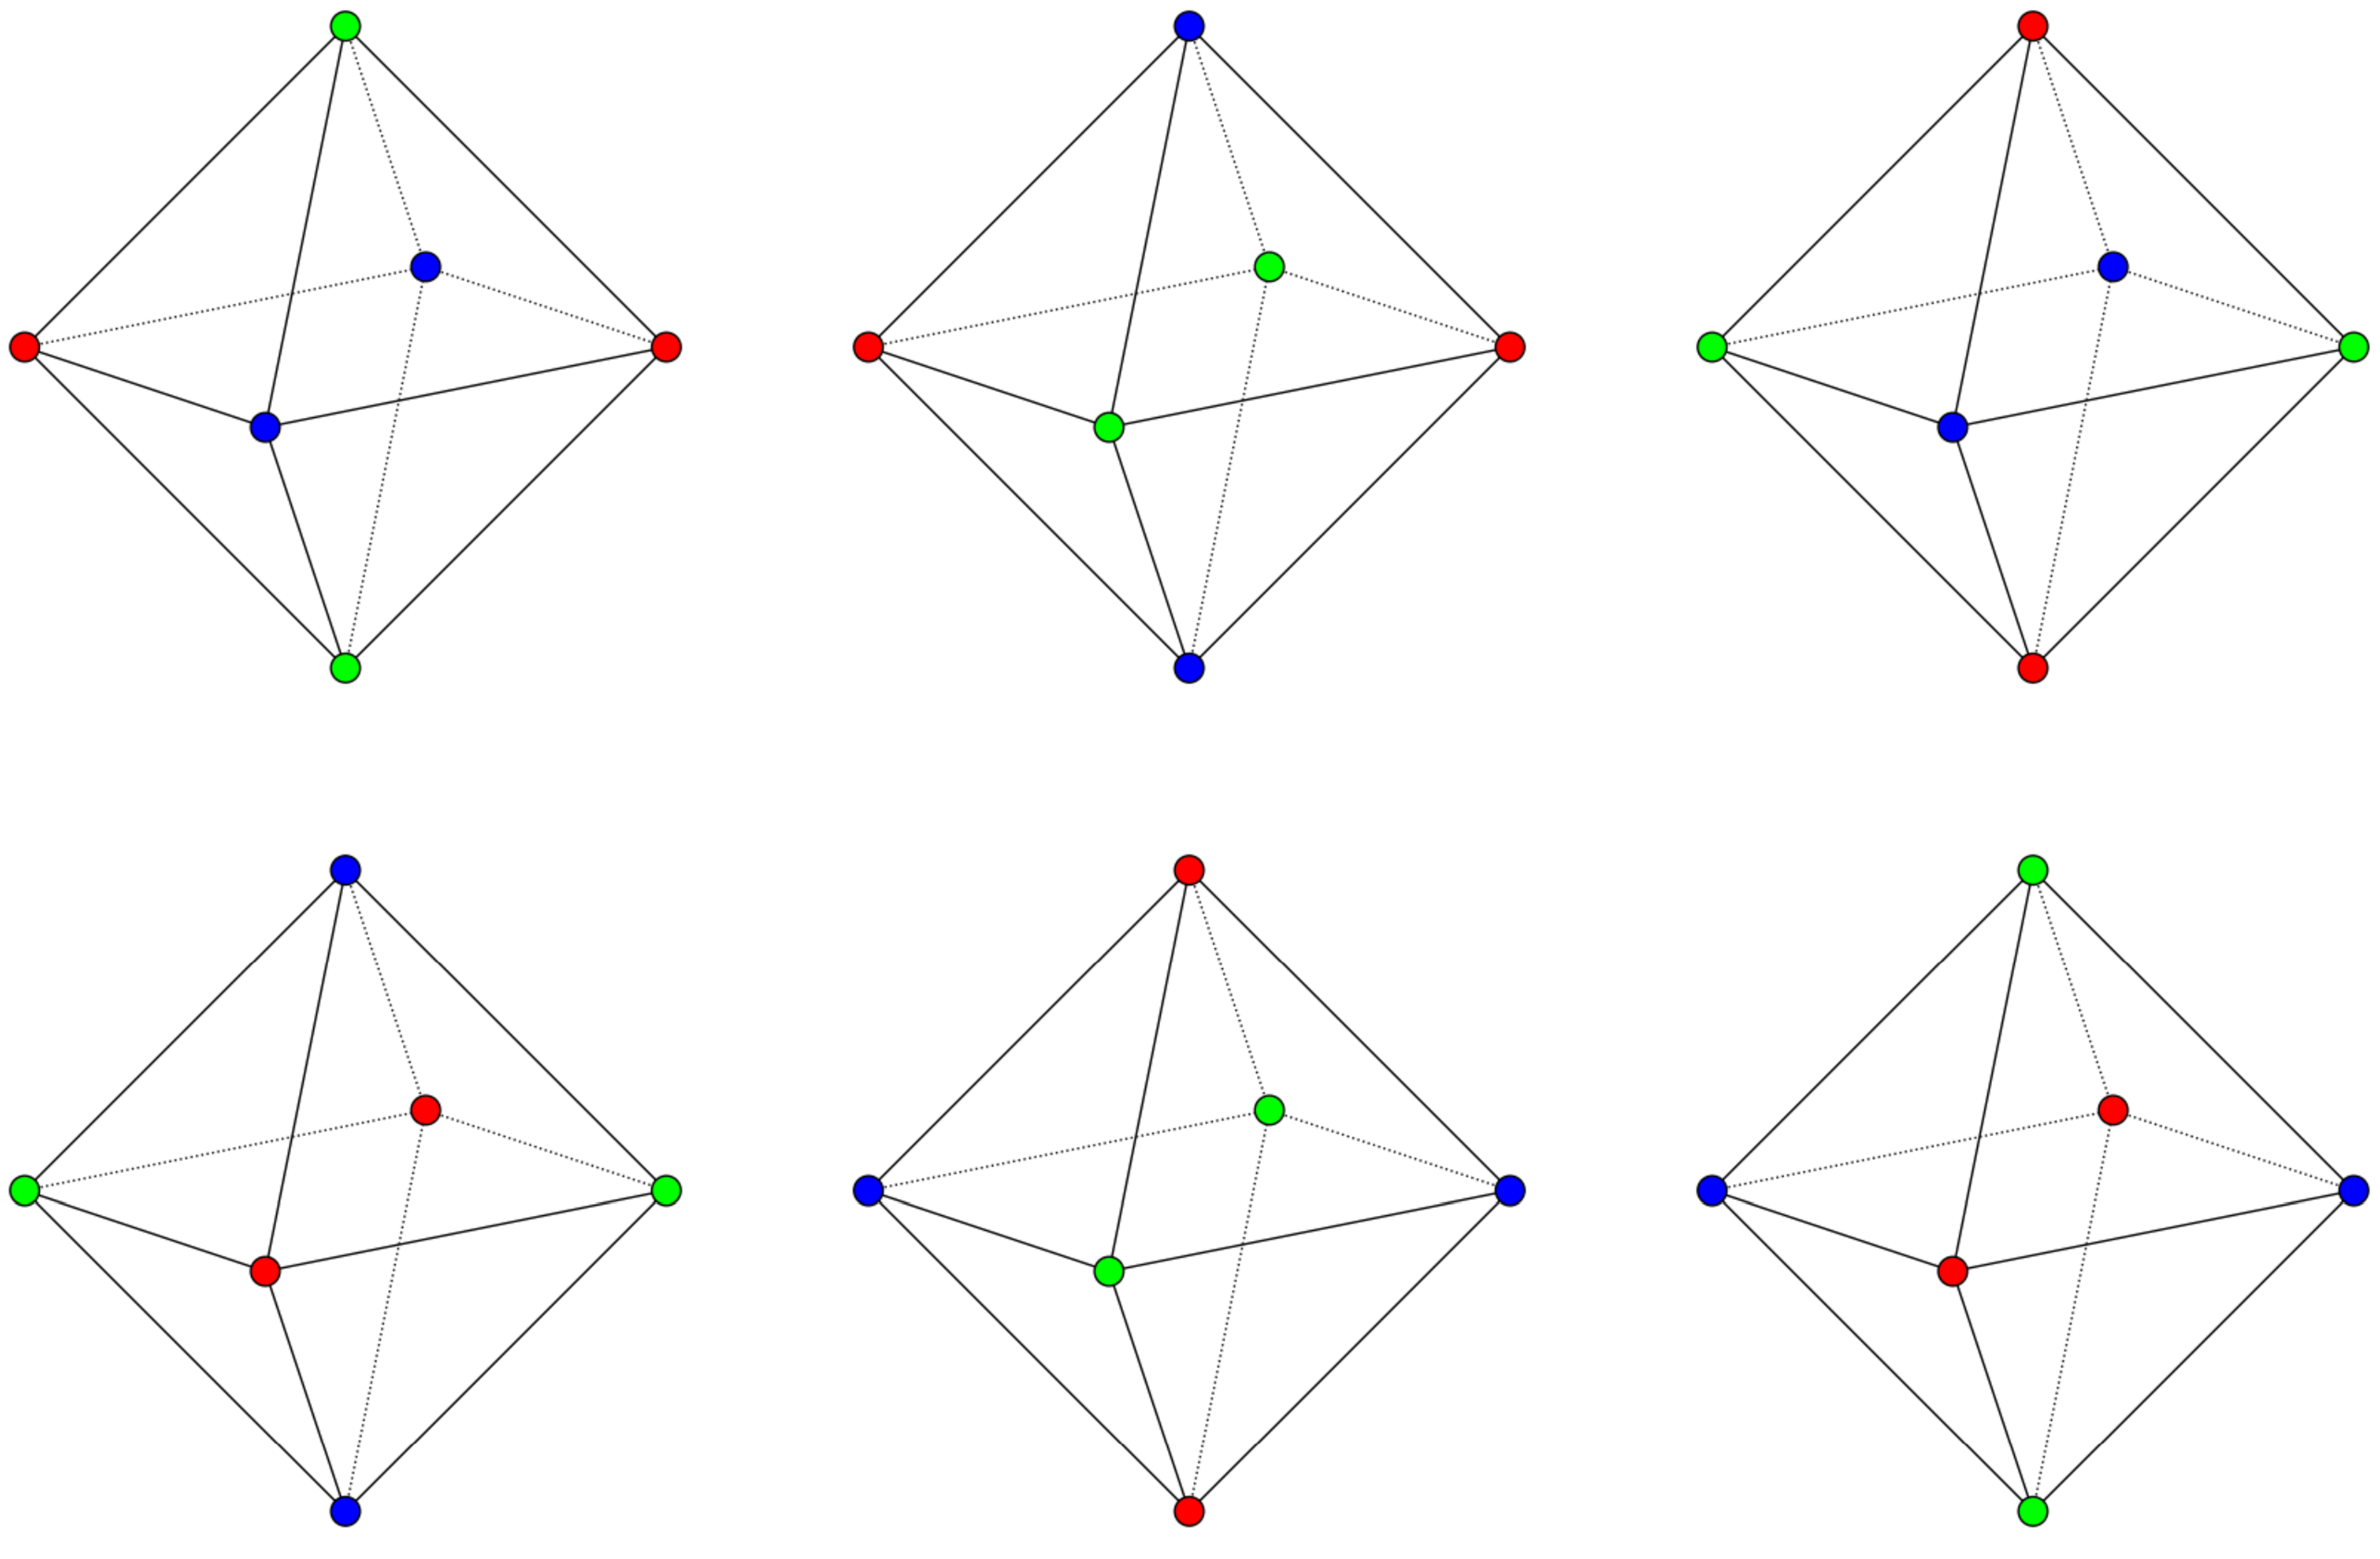
\includegraphics[width=1\textwidth]{../Resources/Figs/octahedron_3-clrings.pdf}
    \caption{All 3 colorings of octahedral graph}
    \label{fig:octahedron-3-clrings}
\end{figure}

Now, an important observation is, that all of these $6$ colorings are equivalent when considered up to automorphisms. Indeed we can compute that $OP(K_{3 \times 2},3) = 1$.

\begin{highlight}

\section{Comparison with chromatic polynomial}

It is interesting to compare the difference between chromatic polynomial and orbital chromatic polynomial for all the solids by looking at the values of the polynomials at certain points. This can be seen in table \ref{tab:platonic-polys-evals} below.

\begin{table}[H]
\centering
\begin{tabular}{l@{\hspace{0.5cm}}ccccccc}
\toprule
\textbf{Platonic solid} & \textbf{2} & \textbf{3} & \textbf{4} & \textbf{5} & \textbf{6} & \textbf{7} & \textbf{8} \\
\midrule
tetrahedron & $0$ & $0$ & $24$ & $120$ & $360$ & $840$ & $1680$ \\
 & $0$ & $0$ & $1$ & $5$ & $15$ & $35$ & $70$ \\
\specialrule{0.2pt}{0.65ex}{0.65ex}
octahedron & $0$ & $6$ & $96$ & $780$ & $4080$ & $15330$ & $45696$ \\
 & $0$ & $1$ & $10$ & $55$ & $215$ & $665$ & $1736$ \\
\specialrule{0.2pt}{0.65ex}{0.65ex}
cube & $2$ & $114$ & $2652$ & $29660$ & $198030$ & $932862$ & $3440024$ \\
 & $1$ & $15$ & $154$ & $1115$ & $5955$ & $24836$ & $85260$ \\
\specialrule{0.2pt}{0.65ex}{0.65ex}
icosahedron & $0$ & $0$ & $240$ & $80400$ & $4012560$ & $\approx 10^{7}$ & $\approx 10^{8}$ \\
 & $0$ & $0$ & $2$ & $670$ & $33444$ & $640444$ & $6878900$ \\
\specialrule{0.2pt}{0.65ex}{0.65ex}
dodecahedron & $0$ & $7200$ & $\approx 10^{8}$ & $\approx 10^{11}$ & $\approx 10^{13}$ & $\approx 10^{14}$ & $\approx 10^{16}$ \\
 & $0$ & $75$ & $1404848$ & $\approx 10^{8}$ & $\approx 10^{11}$ & $\approx 10^{12}$ & $\approx 10^{14}$ \\
\bottomrule
\end{tabular}
\caption{Evaluated chromatic polynomial and orbital chromatic polynomial for platonic solids at points 2 to 8. For each solid, the top row contains the chromatic polynomial, the bottom row contains the orbital chromatic polynoial.}
\label{tab:platonic-polys-evals}
\end{table}

Note we can use the same method as in section \ref{sec:num-clrings-exactly-n-clrs} using the formula \ref{eqn:exactly-n-colors} also for the orbital chromatic polynomial $OP(G,x)$ to arrive at corresponding values $OP^*(G,n)$. Using this formula, we can then simplify table \ref{tab:platonic-polys-evals} above to get the following table:

\begin{table}[H]
\centering
\begin{tabular}{l@{\hspace{0.5cm}}ccccccc}
\toprule
\textbf{Platonic solid} & \textbf{2} & \textbf{3} & \textbf{4} & \textbf{5} & \textbf{6} & \textbf{7} & \textbf{8} \\
\midrule
tetrahedron & $0$ & $0$ & $24$ & $0$ & $0$ & $0$ & $0$ \\
 & $0$ & $0$ & $1$ & $0$ & $0$ & $0$ & $0$ \\
\specialrule{0.2pt}{0.65ex}{0.65ex}
octahedron & $0$ & $6$ & $72$ & $360$ & $720$ & $0$ & $0$ \\
 & $0$ & $1$ & $6$ & $15$ & $15$ & $0$ & $0$ \\
\specialrule{0.2pt}{0.65ex}{0.65ex}
cube & $2$ & $108$ & $2208$ & $17520$ & $57600$ & $80640$ & $40320$ \\
 & $1$ & $12$ & $100$ & $485$ & $1290$ & $1680$ & $840$ \\
\specialrule{0.2pt}{0.65ex}{0.65ex}
icosahedron & $0$ & $0$ & $240$ & $79200$ & $3533760$ & $\approx 10^{7}$ & $\approx 10^{8}$ \\
 & $0$ & $0$ & $2$ & $660$ & $29454$ & $420336$ & $2654400$ \\
\specialrule{0.2pt}{0.65ex}{0.65ex}
dodecahedron & $0$ & $7200$ & $\approx 10^{8}$ & $\approx 10^{11}$ & $\approx 10^{13}$ & $\approx 10^{14}$ & $\approx 10^{16}$ \\
 & $0$ & $75$ & $1404548$ & $\approx 10^{8}$ & $\approx 10^{11}$ & $\approx 10^{12}$ & $\approx 10^{14}$ \\
\bottomrule
\end{tabular}
\caption{Numbers of colorings using exactly 2 to 8 colors. For each solid, the top row contains the value when counting symmetric colorings as different. The bottom row takes two colorings as different only if they cannot be identified using some automorphism.}
\label{tab:platonic-exactly-n-clrs}
\end{table}

\end{highlight}
\chapter{Counting number of partitions into independent sets}
\label{chap:num-partitions-into-indep-sets}

\begin{highlight}



\vtodo{Add visual example of 3-colorings of cube up to automorphisms.}

\section{Counting partitionings into independent sets}

Important thing to note about results of table \ref{tab:platonic-exactly-n-clrs} above is the fact, that we count two colorings $c_1$ and $c_2$ as different also in the case, when $c_1$ can be obtained as a permutation of colors of $c_2$. This is something we would like to avoid if we are interested in the structure of the coloring only and the value of the colors bear no special meaning to us. 

\begin{defn}[relabeling relation]
    Given a graph $G=(V,E)$ and a set of colorings $C$, we define a relation $\leftrightarrow \; \subseteq C \times C$ as follows: For any two colorings $c_1,c_2 \in C$ we have $c_1 \leftrightarrow c_2$ iff exists a permutation of colors $\pi$ s.t. $\forall v \in V : c_1(v) = \pi(c_2(v))$. We call this relation the \emph{relabeling relation}.
\end{defn}

The relabeling relation is in fact an equivalence relation as it is reflexive, symmetric and transitive.

\begin{defn}[number of exact n-partitions]
    Let us for a given $n \in \mathbb{N}$ denote by $P^*_{\leftrightarrow}(G,n)$ the number of equivalence classes of $\leftrightarrow$ on the set of all proper vertex colorings. 
\end{defn}

The equivalence classes in definition above correspond to different partitions of the set $V(G)$ into independent sets irrespectively of the particular colors that we assign the vertices. Note that now, we might still consider two partitions as different even though they can be made equal by applying some automorphism. In order to calculate $P^*_{\leftrightarrow}(G,n)$, consider any partition $W$ of $V(G)$ into independent sets and count how many different colorings correspond to $W$. Because $W$ consists of exactly $n$ independent sets, we have $n!$ possible ways of assigning colors to the independent sets of $W$. As this holds for any arbitrary partition of size $n$, it follows that:
\begin{equation}\label{eqn:count-relabel-orbits}
    P^*_{\leftrightarrow}(G,n) \cdot n! = P^*(G,n)
\end{equation}

Using this formula, we can compute yet another table shown below:

\begin{table}[H]
\centering
\begin{tabular}{l@{\hspace{0.5cm}}ccccccc}
\toprule
\textbf{Platonic solid} & \textbf{2} & \textbf{3} & \textbf{4} & \textbf{5} & \textbf{6} & \textbf{7} & \textbf{8} \\
\midrule
tetrahedron & $0$ & $0$ & $1$ & $0$ & $0$ & $0$ & $0$ \\
octahedron & $0$ & $1$ & $3$ & $3$ & $1$ & $0$ & $0$ \\
cube & $1$ & $18$ & $92$ & $146$ & $80$ & $16$ & $1$ \\
icosahedron & $0$ & $0$ & $10$ & $660$ & $4908$ & $10008$ & $7900$ \\
dodecahedron & $0$ & $1200$ & $7019920$ & $\approx 10^{8}$ & $\approx 10^{10}$ & $\approx 10^{11}$ & $\approx 10^{11}$ \\
\bottomrule
\end{tabular}
\caption{Numbers of of possible partitions of vertices of the graphs into $n$ independent sets.}
\label{tab:platonic-exact-n-partitions}
\end{table}

Notice, that even though we managed to overcome the problem of counting a single partition $W$ of $G$ into independent sets multiple times, because of the ways we can relabel the colorings, the method still suffers from the following: Rotated or reflected independent sets might be counted as different objects. This happens exactly in the cases, when by rotating some partition $W_1$, we arrive at a partition $W_2$ s.t. for any coloring $c_1$ obtained by labeling the sets of $W_1$ and for any coloring $c_2$ obtained by labeling sets of $W_2$ we have $c_1 \not\leftrightarrow c_2$. In other words, we cannot create $c_2$ by renaming the colors of $c_1$ or vice versa.

This problem is illustrated on figure \ref{fig:example-octahedron-4-partitions} below. We can see that all three partitions are same when we allow rotating the solid. But it is impossible to arrive from one coloring to another by simply relabeling the colors. 

\begin{figure}[H]
    \centering
    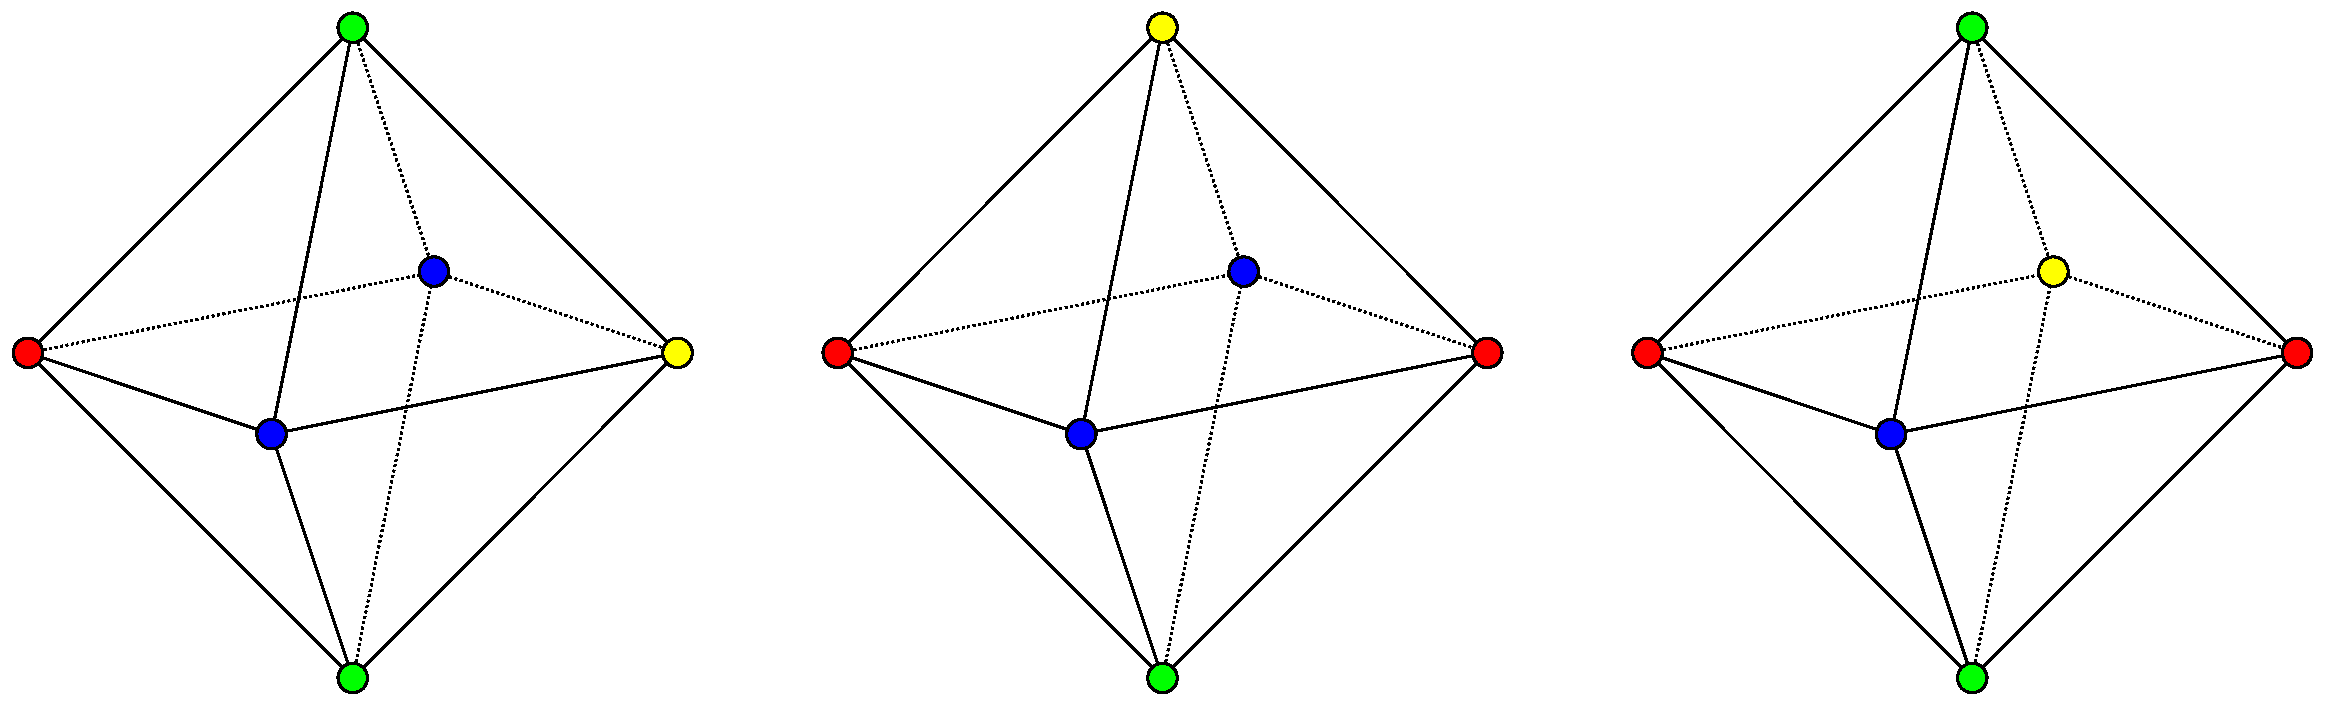
\includegraphics[width=1\textwidth]{Resources/Figs/example-octahedron-4-partitions.pdf}
    \caption{All partitions of octahedron to 4 independent sets. Notice that they are structurally the same partitions when we allow us to rotate the solid.}
    \label{fig:example-octahedron-4-partitions}
\end{figure}

Note that in some cases of symmetric colorings, this problem is avoided. For example, any rotation or reflection of a 4-coloring of tetrahedron can be obtained by simply relabeling the colors as well. See this on the figure below:

\begin{figure}[H]
    \centering
    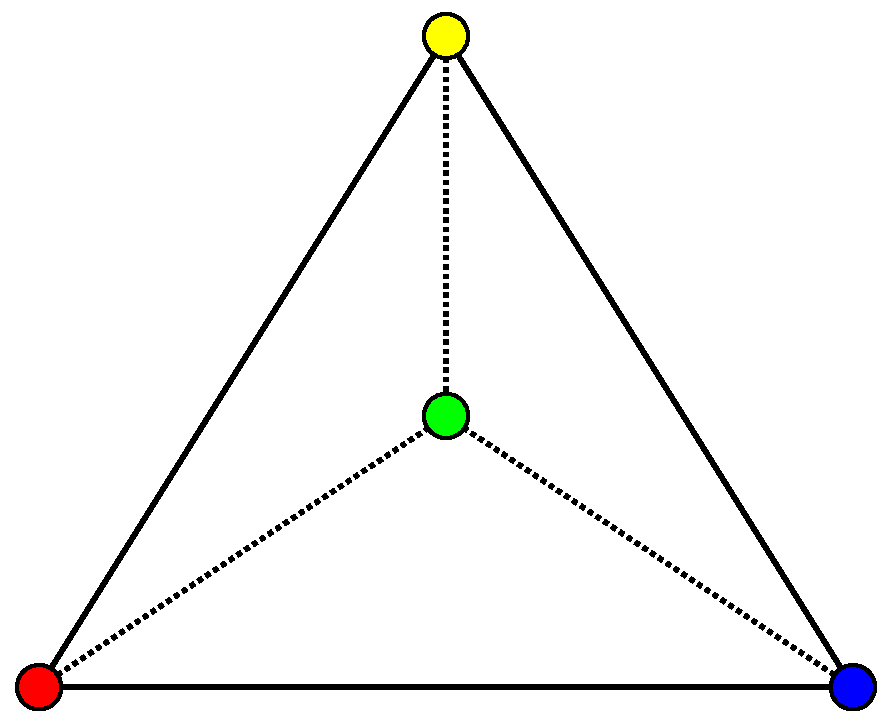
\includegraphics[width=0.3\textwidth]{Resources/Figs/example-tetrahedron-4-clring.pdf}
    \caption{A coloring of tetrahedron using 4 colors. Notice that any rotation of this coloring can be obtained by simply relabeling the colors.}
    \label{fig:example-tetrahedron-4-coloring}
\end{figure}

Overcoming the problem of counting rotations or reflection of the same partition multiple times motivates the following definition:

\begin{defn}[relabeling-automorphism relation]
    Let $G=(V,E)$ be a graph and $C$ a set of its vertex colorings. We define a relation $\rightleftharpoons \; \subseteq C \times C$ as follows: Given two colorings $c_1,c_2 \in C$ we have $c_1 \rightleftharpoons c_2$ iff there exists a permutation of colors $\pi$ and an automorphism $\alpha \in \Aut(G)$ s.t. $\forall v \in V : c_1(v) = \pi(c_2(\alpha(v)))$. We call this relation the \emph{relabeling-automorphism relation}.
\end{defn}

The relabeling-automorphism relation is again an equivalence relation. For reflexivity, we can simply take $\pi = id$ and $\alpha = id$. For symmetry, suppose we have $\pi$ and $\alpha$ s.t. $\forall v \in V : c_1(v) = \pi(c_2(\alpha(v)))$. Suppose we have a $w \in V$, then there exists $v \in V$ s.t. $w = \alpha(v)$. We will show that $c_2(w) = \pi^{-1}(c_1(\alpha^{-1}(w)))$. We can rewrite the previous in form $c_2(\alpha(v)) = \pi^{-1}(c_1(\alpha^{-1}(\alpha(v))))$ which is equivalent to $c_2(\alpha(v)) = \pi^{-1}(c_1(v)) \iff c_1(v) = \pi(c_2(\alpha(v)))$ which holds by the assumption. For transitivity, we have that $\exists \pi, \pi', \alpha ,\alpha'$ s.t. $\forall v \in V : c_1(v) = \pi(c_2(\alpha(v))) \wedge c_2(v) = \pi'(c_3(\alpha'(v)))$ from which we get $c_1(v)=\pi(\pi'(c_3(\alpha'(\alpha(v)))))$. This means that $\pi \circ \pi'$ and $\alpha' \circ \alpha$ are the permutation of colors and automorphism we are looking for.

Since $\rightleftharpoons$ is an equivalence relation, we can again consider its partition into equivalence classes, $C/_\rightleftharpoons$ and count the number of these classes, $\abs{C/_\rightleftharpoons}$. This is be an interesting number to calculate, since if $C$ is the set of n-colorings of graph $G$, then each equivalence class corresponds to a structurally different partitioning of $G$ into $n$ non-empty independent sets.

\begin{defn}[orbital number of exact n-partitions]
    Let us for a given $n \in \mathbb{N}$ denote by $P^*_{\rightleftharpoons}(G,n)$ the number of equivalence classes of $\rightleftharpoons$ on the set of all proper vertex colorings. 
\end{defn}

It is tempting to suppose that $P^*_{\rightleftharpoons}(G,n)$ can be calculated from $OP^*(G,n)$ in a similar fashion as can be $P^*_{\leftrightarrow}(G,n)$ calculated using $P^*(G,n)$ by formula \ref{eqn:count-relabel-orbits}. In that formula, we showed for each equivalence class of $C/_\leftrightarrow$, we count exactly $n!$ colorings in $C$ when we use $P^*(G,n)$. If something similar is to hold for $\rightleftharpoons$, we would have to show that for each equivalence class of $C/_\rightleftharpoons$, we count exactly $k$ equivalence classes of $C/_\sim$ when using $OP^*(G,n)$ for some fixed number $k$. Unfortunately, this is not the case since there exists graph $G$ and a set of its n-colorings $C$ s.t. there are equivalence classes of $C/_\rightleftharpoons$ that are counted exactly once by $OP^*(G,n)$ but also classes that are counted multiple times.

For example consider the graph of cube and its following two 4-colorings:

\begin{figure}[H]
    \centering
    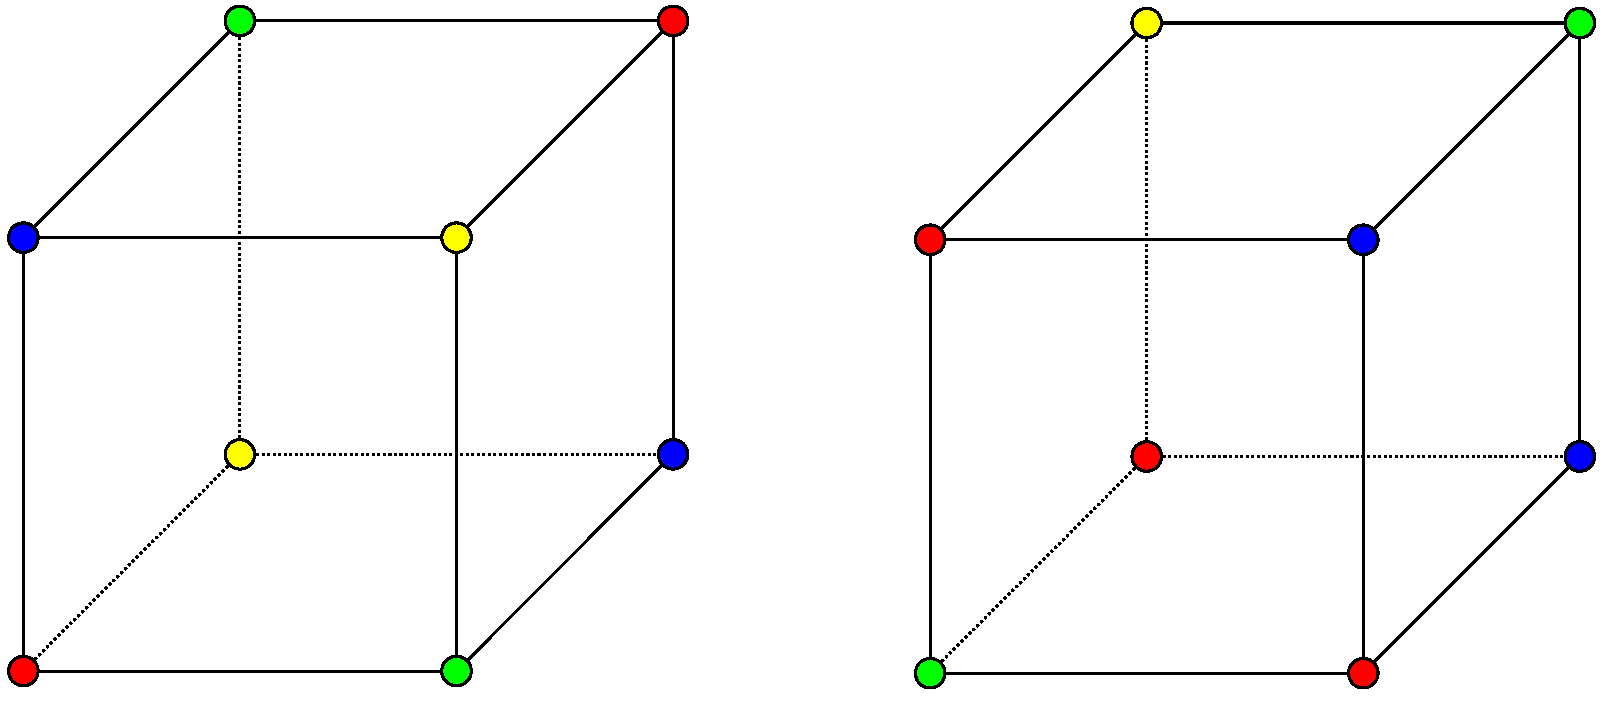
\includegraphics[width=0.75\textwidth]{Resources/Figs/example_diff_rel-aut_class_sizes.pdf}
    \caption{Two structurally different partitions of cube into independent sets.}
    \label{fig:example-cube-4-clrings-diff-classes}
\end{figure}

When the colorings in figure \ref{fig:example-cube-4-clrings-diff-classes} are viewed as a partition, then the left partition represents a single equivalence class of both $\sim$ and $\rightleftharpoons$. This follows from the fact, that permuting the colors of the independent set leads to a coloring, that can be obtained from the original coloring by simply rotating the solid.

On the other hand the partition one the right represents $4!$ equivalence classes of $\sim$ since any permutation of colors yields a different equivalence class of $\sim$.

\section{Bounds on number of equivalence classes of the relabeling-automorphism relation}

Before we show, how the number of equivalence classes of $\rightleftharpoons$ can be computed using a brute force algorithm, we provide bounds on the this number, $P^*_\rightleftharpoons(G,n)$, using the numbers $P^*_\leftrightarrow(G,n)$ and $OP^*(G,n)$.

\begin{claim}\label{clm:relabeling-bound}
    For any graph $G=(V,E)$ and a natural number $n$, we have: $$\frac{1}{\abs{\Aut(G)}} \cdot P^*_\leftrightarrow(G,n) \leq P^*_\rightleftharpoons(G,n) \leq P^*_\leftrightarrow(G,n)$$ 
\end{claim}

\begin{proof}

The inequality $P^*_\rightleftharpoons(G,n) \leq P^*_\leftrightarrow(G,n)$ is simple. It follows from the fact, that for any two colorings $c_1$,$c_2$ of graph $G$, if we have $c_1 \not\rightleftharpoons c_2$, then also $c_1 \not\leftrightarrow c_2$. So there must be at least as many equivalence classes of $\leftrightarrow$ as they are of $\rightleftharpoons$.

For inequality $\frac{1}{\abs{\Aut(G)}} \cdot P^*_\leftrightarrow(G,n) \leq P^*_\rightleftharpoons(G,n)$ we show, that for each equivalence class of $\rightleftharpoons$ there are at most $n!$ equivalence classes of $\leftrightarrow$. Remember that $n$ is the number of colors or independent sets that the colorings of $G$ we consider have. Let $c_1$ be some coloring, that belongs to some equivalence class $E_\rightleftharpoons$ of $\rightleftharpoons$ and equivalence class $E_\leftrightarrow$ of $\leftrightarrow$. All possible relabelings of colors of $c_1$ will be contained in both classes $E_\rightleftharpoons$ and $E_\leftrightarrow$. On the other hand, there exist at most $\abs{\Aut(G)}$ ways to rotate the coloring $c_1$ which will all be contained in $E_\rightleftharpoons$ but may result in at most $\abs{\Aut(G)}$ different equivalence classes of $\leftrightarrow$.

\end{proof}

Notice, that the result of claim $\ref{clm:relabeling-bound}$ gives us equality for any graph $G$ s.t. $\Aut(G) = \{id\}$ i.e. a graph, whose only symmetry is the identity function. In general, the lower bound is higher for graphs that are not very symmetric. Unfortunately, this is not the case for our graphs, so the lower bounds will not give us as much information.

Calculated values using these bounds are shown on table below:

\begin{table}[H]
\centering
\begin{tabular}{l@{\hspace{0.5cm}}ccccccc}
\toprule
\textbf{Platonic solid} & \textbf{2} & \textbf{3} & \textbf{4} & \textbf{5} & \textbf{6} & \textbf{7} & \textbf{8} \\
\midrule
tetrahedron & $0$ & $0$ & $1$ & $0$ & $0$ & $0$ & $0$ \\
 & $0$ & $0$ & $1$ & $0$ & $0$ & $0$ & $0$ \\
\specialrule{0.2pt}{0.65ex}{0.65ex}
octahedron & $0$ & $1$ & $3$ & $3$ & $1$ & $0$ & $0$ \\
 & $0$ & $1$ & $1$ & $1$ & $1$ & $0$ & $0$ \\
\specialrule{0.2pt}{0.65ex}{0.65ex}
cube & $1$ & $18$ & $92$ & $146$ & $80$ & $16$ & $1$ \\
 & $1$ & $1$ & $2$ & $4$ & $2$ & $1$ & $1$ \\
\specialrule{0.2pt}{0.65ex}{0.65ex}
icosahedron & $0$ & $0$ & $10$ & $660$ & $4908$ & $10008$ & $7900$ \\
 & $0$ & $0$ & $1$ & $6$ & $41$ & $84$ & $66$ \\
\specialrule{0.2pt}{0.65ex}{0.65ex}
dodecahedron & $0$ & $1200$ & $7019920$ & $\approx 10^{8}$ & $\approx 10^{10}$ & $\approx 10^{11}$ & $\approx 10^{11}$ \\
 & $0$ & $10$ & $58500$ & $7761169$ & $\approx 10^{8}$ & $\approx 10^{9}$ & $\approx 10^{9}$ \\
\bottomrule
\end{tabular}
\caption{Upper and lower bounds for the number of equivalence classes of the relabeling-automorphism relation based on the number of equivalence classes of the relabeling relation.}
\label{tab:bounds-exactn-n-partitions}
\end{table}

\begin{claim}\label{clm:automorphism-bound}
    For any graph $G=(V,E)$ and a natural number $n$, we have: $$\frac{1}{n!} \cdot OP^*(G,n) \leq P^*_\rightleftharpoons(G,n) \leq OP^*(G,n)$$
\end{claim}

\begin{proof}

Argument for inequality $P^*_\rightleftharpoons(G,n) \leq OP^*(G,n)$ is again simple and analogous to the one in clam \ref{clm:relabeling-bound}. We notice, that if for any two colorings $c_1,c_2$ we have $c_1 \not\rightleftharpoons c_2$ then also $c_1 \not\sim c_2$.

For inequality $\frac{1}{n!} \cdot OP^*(G,n) \leq P^*_\rightleftharpoons(G,n)$ we proceed again analogously as in claim \ref{clm:relabeling-bound}. We show that for each equivalence class of $\rightleftharpoons$ we have at most $n!$ equivalence classes of $\sim$. We imagine a coloring $c_1$ that belongs to some equivalence class $E_\rightleftharpoons$ of $\rightleftharpoons$ and $E_\sim$ of $\sim$. Applying any automorphism $\alpha \in \Aut(G)$ results in a coloring, that will be contained in both $E_\rightleftharpoons$ and $E_\sim$. On the other hand, by relabeling the colors of $c_1$ we may obtain $n!$ colorings s.t. each belongs to a different equivalence class of $\sim$ even though they all belong to $E_\rightleftharpoons$.

\end{proof}

Note, that the lower bound resulting from $\ref{clm:automorphism-bound}$ is useful for cases where $n$, the number of colors, is small. In such cases, it can give us a better bound than what the bound from $\ref{clm:relabeling-bound}$ gives.

See values resulting from this bound in the table below and compare with table \ref{tab:bounds-exactn-n-partitions}.

\begin{table}[H]
\centering
\begin{tabular}{l@{\hspace{0.5cm}}ccccccc}
\toprule
\textbf{Platonic solid} & \textbf{2} & \textbf{3} & \textbf{4} & \textbf{5} & \textbf{6} & \textbf{7} & \textbf{8} \\
\midrule
tetrahedron & $0$ & $0$ & $1$ & $0$ & $0$ & $0$ & $0$ \\
 & $0$ & $0$ & $1$ & $0$ & $0$ & $0$ & $0$ \\
\specialrule{0.2pt}{0.65ex}{0.65ex}
octahedron & $0$ & $1$ & $6$ & $15$ & $15$ & $0$ & $0$ \\
 & $0$ & $1$ & $1$ & $1$ & $1$ & $0$ & $0$ \\
\specialrule{0.2pt}{0.65ex}{0.65ex}
cube & $1$ & $12$ & $100$ & $485$ & $1290$ & $1680$ & $840$ \\
 & $1$ & $2$ & $5$ & $5$ & $2$ & $1$ & $1$ \\
\specialrule{0.2pt}{0.65ex}{0.65ex}
icosahedron & $0$ & $0$ & $2$ & $660$ & $29454$ & $420336$ & $2654400$ \\
 & $0$ & $0$ & $1$ & $6$ & $41$ & $84$ & $66$ \\
\specialrule{0.2pt}{0.65ex}{0.65ex}
dodecahedron & $0$ & $75$ & $1404548$ & $\approx 10^{8}$ & $\approx 10^{11}$ & $\approx 10^{12}$ & $\approx 10^{14}$ \\
 & $0$ & $13$ & $58523$ & $7761220$ & $\approx 10^{8}$ & $\approx 10^{9}$ & $\approx 10^{9}$ \\
\bottomrule
\end{tabular}
\caption{Upper and lower bounds for the number of equivalence classes of the relabeling-automorphism relation based on the number of equivalence classes of the $\sim$ relation.}
\label{tab:bounds-orbital}
\end{table}

\section{Algorithm for computing number of equivalence classes of the relabeling-automorphism relation}

\vtodo{Describe the algorithm for computing equivalence classes of $\rightleftharpoons$}

\vtodo{Demonstrate results of using this algorithm}

\end{highlight}
\chapter*{Conclusion}
\addcontentsline{toc}{chapter}{Conclusion}

\begin{highlight}

In this thesis, we studied various coloring problems on graphs of Platonic and Archimedean solids. Firstly, we studied, what general properties graphs of these solids have and then continued by defining various concepts of coloring, that can be applied on those graphs.

Before delving into details about the particular types of colorings, we generalized the concept of coloring, which ties all the specific types of colorings together. For the particular cases, we also provided examples of these colorings on selected Platonic graphs and later showed connections that exist between some of the colorings.

Then, we continued by computing chromatic numbers for selected types of colorings, while exploiting the conversions between some of the colorings defined before. We studied chromatic polynomials of the solids and found an explicit formula for calculating chromatic polynomials of k-partite graphs with partite size 2. Graph of the octahedron is an example of such graph.

After considering limitations of the chromatic polynomial, we studied the concept of orbital chromatic polynomial, which allows for computing numbers of colorings up to symmetries. We implemented an algorithm for computing this polynomial based on an approach suggested by P.J. Cameron. This algorithm is then used to compute this polynomial for all Platonic and selected Archimedean solids.

In following section, we addressed a second limitation of the standard chromatic polynomial. Namely, we showed a method for calculating the number of colorings, when they are viewed only as partitions into independent sets irrespective of values of the colors that the sets receive.

We then showed that combining the methods above to calculate number of independent sets up to symmetries is not trivial and provided some bounds on the desired numbers. Finally, we provide an algorithm that computes these numbers by enumerating all the colorings and then filtering them. We also provide illustrations of the colorings that were counted by the algorithm. Finding a better method or a more effective algorithm is a problem we leave unanswered.

We studied all the topics, starting with the chromatic polynomial and going till the end of the thesis, for vertex coloring only. This was intentional, since as we previously showed, we can use standard conversions to solve the problems for most of the other mentioned particular colorings. On the other hand, for rainbow coloring and magic labeling, we leave the door open for further investigation in the future.

\end{highlight}

%%% Bibliography
%%% Seznam použité literatury je zpracován podle platných standardů. Povinnou citační
%%% normou pro bakalářskou práci je ISO 690. Jména časopisů lze uvádět zkráceně, ale jen
%%% v kodifikované podobě. Všechny použité zdroje a prameny musí být řádně citovány.

\def\bibname{Bibliography}
\begin{thebibliography}{99}
\addcontentsline{toc}{chapter}{\bibname}

\bibitem{lamport94}
  {\sc Lamport,} Leslie.
  \emph{\LaTeX: A Document Preparation System}.
  2. vydání.
  Massachusetts: Addison Wesley, 1994.
  ISBN 0-201-52983-1.

\end{thebibliography}


%%% Figures used in the thesis (consider if this is needed)
\listoffigures

%%% Tables used in the thesis (consider if this is needed)
%%% In mathematical theses, it could be better to move the list of tables to the beginning of the thesis.
\listoftables

%%% Abbreviations used in the thesis, if any, including their explanation
%%% In mathematical theses, it could be better to move the list of abbreviations to the beginning of the thesis.
% \chapwithtoc{List of Abbreviations}

%%% Doctoral theses must contain a list of author's publications
\ifx\ThesisType\TypePhD
\chapwithtoc{List of Publications}
\fi

%%% Attachments to the thesis, if any. Each attachment must be referred to
%%% at least once from the text of the thesis. Attachments are numbered.
%%%
%%% The printed version should preferably contain attachments, which can be
%%% read (additional tables and charts, supplementary text, examples of
%%% program output, etc.). The electronic version is more suited for attachments
%%% which will likely be used in an electronic form rather than read (program
%%% source code, data files, interactive charts, etc.). Electronic attachments
%%% should be uploaded to SIS. Allowed file formats are specified in provision
%%% of the rector no. 72/2017. Exceptions can be approved by faculty's coordinator.
\appendix

\chapter{Attachments}

\begin{highlight}
\section{Tables of calculated chromatic polynomials}\label{sec:more-chrompolys}

\begin{table}[H]
\centering
\scriptsize
\begin{tabular}{cccccc}
\toprule
\textbf{Power of \( x \)} & \textbf{Tetrahedron} & \textbf{Octahedron} & \textbf{Cube} & \textbf{Icosahedron} & \textbf{Dodecahedron} \\
\midrule
\textbf{20} &  &  &  &  & 1 \\
\textbf{19} &  &  &  &  & -30 \\
\textbf{18} &  &  &  &  & 435 \\
\textbf{17} &  &  &  &  & -4060 \\
\textbf{16} &  &  &  &  & 27393 \\
\textbf{15} &  &  &  &  & -142194 \\
\textbf{14} &  &  &  &  & 589875 \\
\textbf{13} &  &  &  &  & -2004600 \\
\textbf{12} &  &  &  & 1 & 5673571 \\
\textbf{11} &  &  &  & -30 & -13518806 \\
\textbf{10} &  &  &  & 415 & 27292965 \\
\textbf{ 9} &  &  &  & -3500 & -46805540 \\
\textbf{ 8} &  &  & 1 & 20023 & 68090965 \\
\textbf{ 7} &  &  & -12 & -81622 & -83530946 \\
\textbf{ 6} &  & 1 & 66 & 241605 & 85371335 \\
\textbf{ 5} &  & -12 & -214 & -517360 & -71159652 \\
\textbf{ 4} & 1 & 58 & 441 & 780286 & 46655060 \\
\textbf{ 3} & -6 & -137 & -572 & -782108 & -22594964 \\
\textbf{ 2} & 11 & 154 & 423 & 463310 & 7171160 \\
\textbf{ 1} & -6 & -64 & -133 & -121020 & -1111968 \\
\bottomrule
\end{tabular}
\caption{Coefficients of chromatic polynomials of Platonic solids, ordered by powers of \( x \).}
\label{tab:chromatic-polys-coefs}
\end{table}
\begin{table}[H]
\centering
\begin{tabular}{lp{0.6\linewidth}}
\toprule
\textbf{Archimedean} & \textbf{Chromatic polynomial} \\
\midrule
trunc. tetrahedron & $x^{12} - 18x^{11} + 149x^{10} - 752x^{9} + 2586x^{8} - 6408x^{7} + 11774x^{6} - 16189x^{5} + 16468x^{4} - 11869x^{3} + 5442x^{2} - 1184x$ \\
cuboctahedron & $x^{12} - 24x^{11} + 268x^{10} - 1842x^{9} + 8680x^{8} - 29516x^{7} + 74019x^{6} - 136826x^{5} + 182024x^{4} - 164656x^{3} + 90016x^{2} - 22144x$ \\
trunc. cube & $x^{24} - 36x^{23} + 622x^{22} - 6868x^{21} + 54445x^{20} - 330016x^{19} + 1590616x^{18} - 6258826x^{17} + 20483524x^{16} - 56517092x^{15} + 132781696x^{14} - 267560902x^{13} + 464751928x^{12} - 698041384x^{11} + 907685011x^{10} - 1021028578x^{9} + 990348490x^{8} - 822946048x^{7} + 579284763x^{6} - 338935770x^{5} + 159596344x^{4} - 57088336x^{3} + 13839584x^{2} - 1703168x$ \\
trunc. octahedron & $x^{24} - 36x^{23} + 630x^{22} - 7134x^{21} + 58707x^{20} - 373816x^{19} + 1914823x^{18} - 8098890x^{17} + 28806937x^{16} - 87308340x^{15} + 227623087x^{14} - 513887650x^{13} + 1008990864x^{12} - 1726780052x^{11} + 2576178723x^{10} - 3343211267x^{9} + 3755216148x^{8} - 3618864524x^{7} + 2949553512x^{6} - 1987203924x^{5} + 1066396109x^{4} - 427989031x^{3} + 114056146x^{2} - 15071023x$ \\
\bottomrule
\end{tabular}
\caption{Chromatic polynomials of some of the Archimedean solids.}
\label{tab:chromatic-polys-some-archs}
\end{table}

\end{highlight}


\section{Size of automorphism groups of Platonic and Archimedean graphs}

\begin{table}[H]
\centering
\begin{tabular}{l@{\hspace{1.5cm}}c}
\toprule
\textbf{Platonic} & \textbf{$\abs{\Aut(G)}$} \\
\midrule
tetrahedron & 24 \\
octahedron & 48 \\
cube & 48 \\
icosahedron & 120 \\
dodecahedron & 120 \\
\bottomrule
\end{tabular}
\caption{Sizes of automorphism groups of graphs of Platonic solids.}
\label{tab:plat-automorphisms}
\end{table}

\begin{table}[H]
\centering
\begin{tabular}{l@{\hspace{1.5cm}}c}
\toprule
\textbf{Archimedean} & \textbf{$\abs{\Aut(G)}$} \\
\midrule
truncated tetrahedron & 24 \\
cuboctahedron & 48 \\
truncated cube & 48 \\
truncated octahedron & 48 \\
rhombicuboctahedron & 48 \\
snub cube & 24 \\
icosidodecahedron & 120 \\
truncated cuboctahedron & 48 \\
truncated icosahedron & 120 \\
truncated dodecahedron & 120 \\
rhombicosidodecahedron & 120 \\
snub dodecahedron & 60 \\
truncated icosidodecahedron & 120 \\
\bottomrule
\end{tabular}
\caption{Sizes of automorphism groups of graphs of Archimedean solids.}
\label{tab:arch-automorphisms}
\end{table}



\section{SageMath programs}

\begin{listing}[H]
\caption{Python implementation of algorithm \ref{alg:orb-chrompoly}}
\begin{lstlisting}
def orbital_chromatic_polynomial(g : Graph):  
    R = PolynomialRing(ZZ, 'x')
    p = R(0)
    A = g.automorphism_group()
    for a in A:
        cycles = a.cycle_tuples()
        if not all([g.is_independent_set(c) for c in cycles]):
            continue
        merged = g.copy()
        for c in cycles:
            merged.merge_vertices(c)
        p += merged.chromatic_polynomial()
    p = p / A.order()
    return p
\end{lstlisting}
\label{prg:orb-chrompoly}
\end{listing}

\end{document}
